% -*- mode: LaTeX -*-
% Customizable fields and text areas start with % >> below.
% Lines starting with the comment character (%) are normally removed before release outside the collaboration, but not those comments ending lines

% svn info. These are modified by svn at checkout time.
% The last version of these macros found before the maketitle will be the one on the front page,
% so only the main file is tracked.
% Do not edit by hand!
\RCS$Revision: 154959 $
\RCS$HeadURL: svn+ssh://svn.cern.ch/reps/tdr2/notes/AN-12-368/trunk/AN-12-368.tex $
\RCS$Id: AN-12-368.tex 154959 2012-10-26 23:32:36Z dudero $

%%%%%%%%%%%%% local definitions %%%%%%%%%%%%%%%%%%%%%
% This allows for switching between one column and two column (cms@external) layouts
% The widths should  be modified for your particular figures. You'll need additional copies if you have more than one standard figure size.
\newlength\cmsFigWidth
\ifthenelse{\boolean{cms@external}}{\setlength\cmsFigWidth{0.85\columnwidth}}{\setlength\cmsFigWidth{0.4\textwidth}}
\ifthenelse{\boolean{cms@external}}{\providecommand{\cmsLeft}{top}}{\providecommand{\cmsLeft}{left}}
\ifthenelse{\boolean{cms@external}}{\providecommand{\cmsRight}{bottom}}{\providecommand{\cmsRight}{right}}

%%%%%%%%%%%%%%%  Title page %%%%%%%%%%%%%%%%%%%%%%%%
\cmsNoteHeader{AN-12-368} % This is over-written in the CMS environment: useful as preprint no. for export versions
% >> Title: please make sure that the non-TeX equivalent is in PDFTitle below
\title{Search for the Standard Model Higgs boson in the $ H \rightarrow WW \rightarrow l\nu jj $ decay with 2012 data}

% >> Authors
%Author is always "The CMS Collaboration" for PAS and papers, so author, etc, below will be ignored in those cases
%For multiple affiliations, create an address entry for the combination
\address[ttu]{Texas Tech University, Lubbock, Texas, USA}
\address[fnal]{Fermi National Accelerator Laboratory, Batavia, Illinois, USA}
\address[mib]{Milano-Bicocca University and INFN, Milan, Italy}
\address[uva]{University of Virginia, Charlottesville, Virginia, USA}
\address[wsu]{Wayne State University, Detroit, Michigan, USA}
\address[tamu]{Texas A\&M University, College Station, Texas, USA}
\address[del]{Delhi University, Delhi, India} 
\address[nebr]{University of Nebraska at Lincoln, Nebraska, USA}
\address[und]{University of Notre Dame, Notre Dame, Indiana, USA}
\address[uerj]{Universidade do Estado do Rio de Janeiro (UERJ), Brazil}
\address[pku]{Peking University, China}
\address[cern]{CERN}
\address[princ]{Princeton Unversity, New Jersey, USA}


\author[ttu]{Nural~Akchurin}
\author[fnal]{Jake~Anderson}
\author[pku]{Chayanit~Asawatangtrakuldee} 
\author[mib]{Andrea~Benaglia}
\author[fnal]{Andrew Beretvas}
\author[fnal]{Jeffrey~Berryhill} 
\author[fnal]{Pushpa~Bhat} 
\author[uva]{Sarah~Boutle}
\author[wsu]{Chris~Clarke} 
\author[mib]{Fabio~Colombo}
\author[uerj]{Analu~Custodio}
\author[ttu]{Jordan~Damgov}
\author[mib]{Leonardo~Di~Matteo}
\author[ttu]{Phil~Dudero}
\author[tamu]{Ricardo~Eusebi} 
\author[cern]{Pietro~Govoni}
\author[fnal]{Dan~Green}
\author[uva]{Joey~Goodell}
\author[wsu]{Robert~Harr} 
\author[princ]{Pratima~Jindal}
\author[del]{Ajay Kumar} 
\author[wsu]{Kristina~Krylova}
\author[und]{Kevin~Lannon} 
\author[ttu]{Sung-Won~Lee}
\author[pku]{Qiang~Li}
\author[pku]{Shuai~Liu}
\author[und]{Wuming~Luo} 
\author[pku]{Yajun~Mao} 
\author[wsu]{Kellen~McGee} 
\author[fnal]{Kalanand~Mishra}
\author[del]{Md.~Naimuddin} 
\author[uva]{Chris~Neu}
\author[tamu]{Ilya~Osipenkov}
\author[tamu]{Alexx~Perloff} 
\author[del]{Kirti~Ranjan} 
\author[wsu]{Sasha~Sakharov}
\author[del]{Ram K Shivpuri}
\author[wsu]{Kevin~Siehl} 
\author[uerj]{Andre~Sznajder}
\author[fnal]{Nhan~V.~Tran}
\author[pku]{Zijun~Xu} 
\author[fnal]{Weimin Wu} 
\author[uva]{John~Wood} 
\author[fnal]{Fan~Yang}
\author[fnal]{Francisco~Yumiceva} 
\author[pku]{Wei~Zou} 

% useful shortcuts
%\renewcommand{\LUMI}{4.7~fb$^{-1}$} %THIS LATEX THING BY NOW DOES NOT WORK

% >> Date
% The date is in yyyy/mm/dd format. Today has been
% redefined to match, but if the date needs to be fixed, please write it in this fashion.
% For papers and PAS, \today is taken as the date the head file (this one) was last modified according to svn: see the RCS Id string above.
% For the final version it is best to "touch" the head file to make sure it has the latest date.
\date{\today}

\abstract{ This note describes the search strategy for the Higgs boson
in the H$\to$WW$\to\ell\nu jj$ final state.  The results are based on
a data sample corresponding to an integrated luminosity of
12~fb$^{-1}$ of proton-proton collisions
accumulated during the 2012A/B/C LHC run, at the
center-of-mass energy of $\sqrt{s}=8\TeV$.}

\hypersetup{%
pdfauthor={L. Di Matteo, P. Dudero},%
pdftitle={Search for the Standard Model Higgs boson in the  H rightarrow WW rightarrow lnu jj  decay with 2012 data},%
pdfsubject={CMS},%
pdfkeywords={CMS, physics, software, computing}}

\maketitle %maketitle comes after all the front information has been supplied

%%%%%%%%%%%%%%%%%%%%%%%%%%%%%%%%  Begin text %%%%%%%%%%%%%%%%%%%%%%%%%%%%%
%% **DO NOT REMOVE THE BIBLIOGRAPHY** which is located before the appendix.
%% You can take the text between here and the bibiliography as an example which you should replace with the actual text of your document.
%% If you include other TeX files, be sure to use "\input{filename}" rather than "\input filename".
%% The latter works for you, but our parser looks for the braces and will break when uploading the document.
%%%%%%%%%%%%%%%s

\tableofcontents
\clearpage{}
\section{Introduction}
\label{sec:intro}
% ---- ---- ---- ---- ---- ---- ---- ---- ---- ---- ---- ---- ---- ---- ---- ---- ---- ---- ---- ---- ---- ---- ----

The Standard Model (SM) of particle physics successfully describes the majority of high-energy
experimental data~\cite{pdg}. One of the key remaining questions is the origin of the masses of
W and Z bosons.  In the simplest implementation of the SM, it is attributed to the spontaneous
breaking of electroweak symmetry caused by a new scalar field. %~\cite{Higgs1, Higgs2, Higgs3} 
The existence of the associated field quantum, the Higgs boson, has yet to be experimentally confirmed.
Therefore, the search for the Higgs boson is arguably one of the most
important studies being done at the LHC~\cite{lhcmachine}. For Higgs
masses above or near the threshold for decay into two vector bosons,
the decay modes of choice are dominated by those decays because of
their large branching fractions.
It is clear that the events where one $W$ decays leptonically, which
provides the main trigger elements, while the other decays
hadronically have the second highest branching fraction and have a
reconstructable Higgs mass peak~\cite{intro2}. 

This note contains the analysis that sets a limit on the Higgs boson cross-section
based on this decay mode, 
performed on the 2012 data acquired by CMS at $\sqrt{s}~=$~8~TeV,
following the same procedures applied for the analysis of 2011 data \cite{HIG-12-003}.
The analysis selects events with one well identified and isolated lepton, 
large missing transverse energy and at least two high \pt jets.
Therefore, the main experimental issue is to control the large $W$ plus jets 
background sufficiently well that the advantages of using this 
final state are realized.

With respect to the 2011 analysis, 
the available sample is acquired this year by single lepton triggers, 
allowing to relax the selection on the tranverse mass of the leptonic W boson.
Physics objects are selected with the techniques available in 2012, 
in particular jet identification is applied to reduce the effect of pile-up.
% The likelihood based analysis applies a b-veto on the third jet, 
% in the case of three jets events, 
% while the fit-based analysis is being implemented after a selection on the most discriminating variables
% of the likelihood training.
The theoretical description of the Higgs lineshape 
follows the recommendation from the Higgs Cross Section Working Group \cite{Dittmaier:2012vm},
therefore the theoretical error has additional components related to the exclusive
segregation of events into separate jet bins.

The note is structured as follows. 
A discussion about the data samples used in the analysis and the trigger selections
is presented in Sections~\ref{sec:MCexpectations} and \ref{sec:technicalities}.  
The physics objects reconstruction is discussed in Section~\ref{sec:firstStep}.
The lepton selection and other preselection requirements are described in detail 
in Section~\ref{sec:firstStep} and \ref{sec:dataMCcomparisons}.

%% A first limit extraction is performed with a few set of selections applied on top of these,
%% as described in Section~\ref{sec:firstExtraction}.
%% To enhance the exclusion power of this analysis, 
%% tighter selections are put in place.

After the preselections,
the signal-over-background ratio is enhanced by means of a selection on a MVA discriminant, 
designed in order to control the background while preserving as much as possible the difference in shape
with respect to the signal (Section~\ref{sec:mvaoptimization}).
The input variables of the MVA exploit the decay angles of the four-body mass system, 
the kinematics of the entire four-body system. For high mass points, a quark-gluon discriminating
variable, already exploited in the CMS search for a Standard Model Higgs boson in its $\ell{}\ell{}jj$ decay,
is also used in parallel with the MVA discriminant.
The MVA variable definition is optimized with dedicated trainings for each Higgs mass hypothesis case, 
for each lepton flavour ($e$, $\mu$) and for each jets multiplicity (2 jets, 3 jets) independently.
In this way, 48 different configurations are obtained.

The main background contaminating the signal region is W+jets.
Its $m_{\ell{}\nu{}jj}$ shape is extrapolated from sidebands in the $m_{jj}$ distribution 
through Monte Carlo based factors (Section~\ref{sec:wjetsBackground}).
Also the QCD shapes come from a data-driven determination, as described in Section~\ref{sec:dataDrivenQCD}.
The remaining background shapes come from the Monte Carlo.
The normalization of the backgrounds in the signal region 
is measured by fitting their Monte Carlo shapes on the same sidebands in the $m_{jj}$ variable 
(Section~\ref{sec:mjjfitfornormal}).
The determination of the $m_{jj}$ distribution for W+jets is described in Section~\ref{sec:wjetsShape}.

The systematic uncertainties present in the signal description are described in Section~\ref{sec:systematics}.
Section~\ref{sec:limitExtraction} describes the obtained limits on the Standard Model Higgs cross section
and Section~\ref{sec:conclusions} closes this work.

               % motivations and brief description of the note  
\section{Signal and background expectations}
\label{sec:MCexpectations}
% ---- ---- ---- ---- ---- ---- ---- ---- ---- ---- ---- ---- ---- ---- ---- ---- ---- ---- ---- ---- ---- ---- ----


\subsection {The signal}
% .... .... .... .... .... .... .... .... .... .... .... .... .... .... .... .... .... .... .... .... .... .... ....


Figure~\ref{fig:higgsXSBR} shows the trend of the Higgs production cross section and decay branching ratio into four fermions, 
as a function of its mass.
%
\begin{figure}[htb] 
  {\centering
    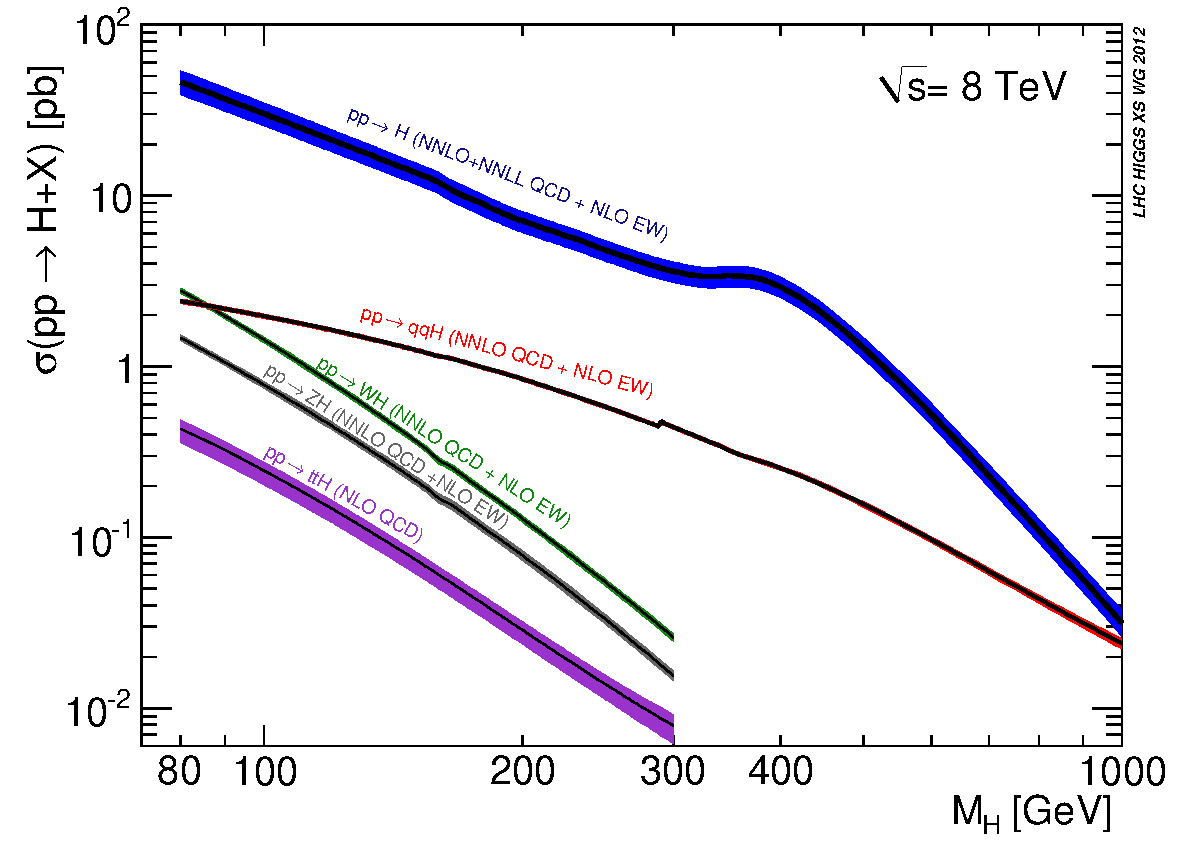
\includegraphics[width=0.54\textwidth]{plots/limitplot/Higgs_XS_8TeV.pdf}
    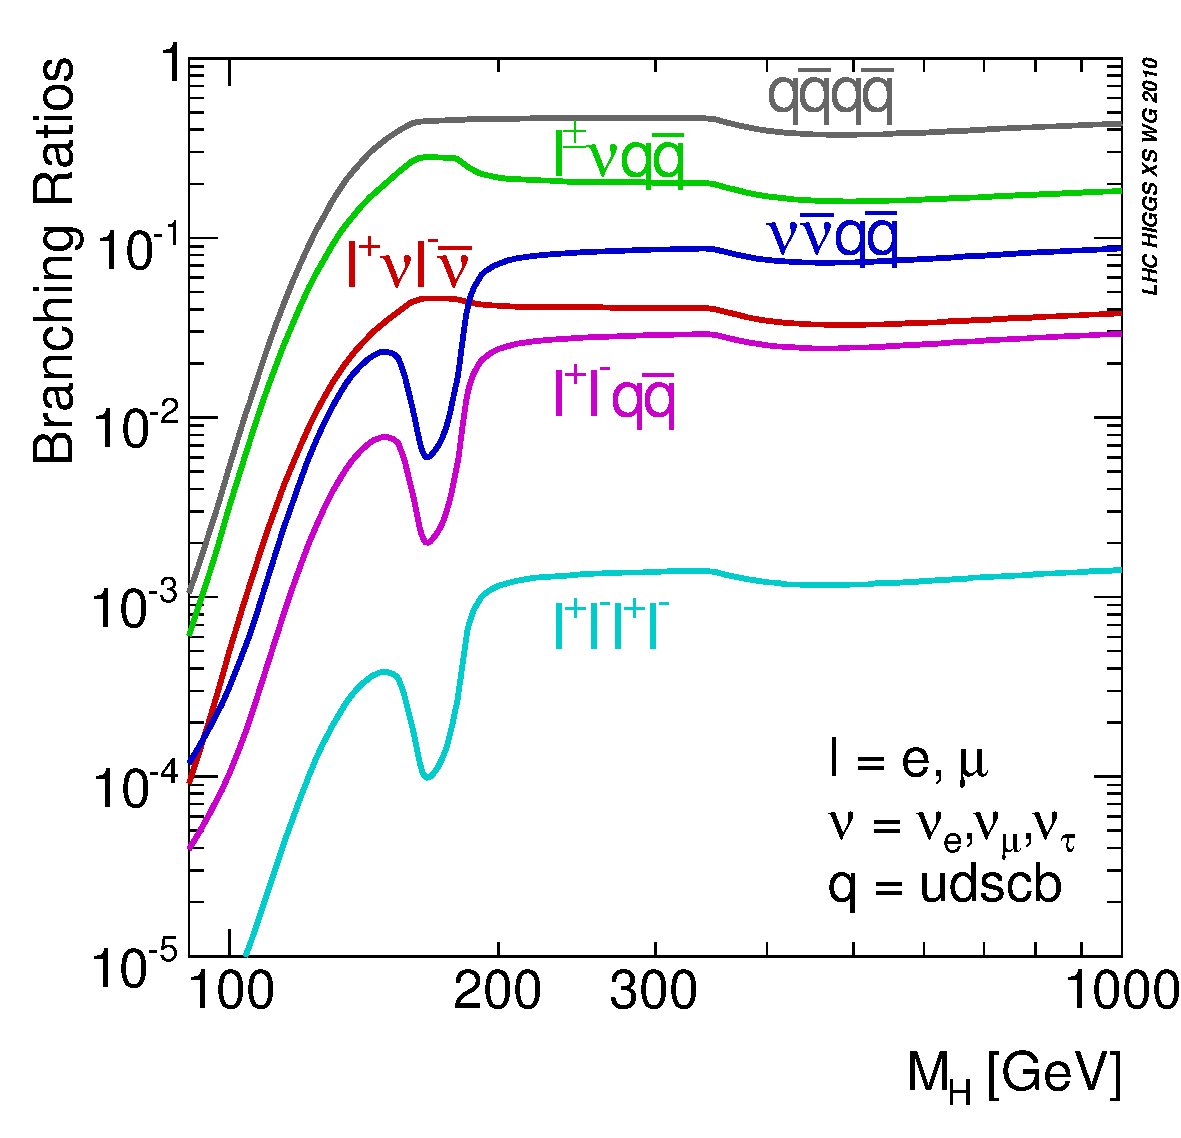
\includegraphics[width=0.42\textwidth]{plots/limitplot/Higgs_BR_4fermion_1.pdf}
    \caption{Standard Model Higgs boson production cross sections at 8TeV (left) and branching ratio into four fermion final states (right).}
    \label{fig:higgsXSBR}}
\end{figure}
%
The inclusive cross-sections used for the Higgs signal at 8~TeV
center-of-mass energy have been calculated by the Higgs Cross Section
Working Group
\cite{LHCHiggsCrossSectionWorkingGroup:2011ti},\cite{Dittmaier:2012vm}
for the gluon-gluon fusion (ggF) and vector boson fusion (VBF)
processes.  All values are taken from \cite{cite:higgsxsecbr}.


\subsection {The backgrounds}
% .... .... .... .... .... .... .... .... .... .... .... .... .... .... .... .... .... .... .... .... .... .... ....


All the processes with the presence in the detector of one lepton, two jets and missing energy
have to be considered as possible sources of background. The most relevant ones are:
% %FIXME in what order should we present it?
\begin{itemize}
  \item $W$+jets: this is the production of single $W$ vector bosons in association with quarks or gluons 
       that mimick the final state signature and the hadronic $W$ decay products.
       Because of its cross-section, 
       this is by far the most important background to the analysis.
  \item Drell-Yan $Z/\gamma^{*}$+jets: this is the production of single $Z/\gamma^{*}$ bosons 
       in association with quarks or gluons, 
       where one lepton gets undetected because of acceptance or inefficiency effects, 
       and the hadronic activity mimicks the final state signature and the hadronic $W$ decay products.
       %FIXME One of the main handles to reduce this background is the low missing energy, the MZZ
  \item $WW$: this non resonant production is an irreducible background for the analysis.
  \item $WZ$: in case the $Z$ decays hadronically, or the $W$ decays hadronically 
              and one $Z$ lepton is not identified by the detector,
              this sample also contributes to the backgrounds.
  \item $ZZ$: in case one $Z$ decays hadronically, and one lepton is not identified by the detector,
              this sample contributes to the backgrounds.
  \item $t\bar{t}$: top quark pairs are produced at LHC via the gluon fusion process
              $gg\to{}t\bar{t}$ or via QCD quark annihilation $qq\to{}t\bar{t}$.
              The semi-leptonic sample, where one $W$ decays hadronically,
              can be reduced by requests on the number of jets,
              while the fully leptonic one is reduced by requiring only one good lepton in the event.
              In any case, 
              because of acceptance and inefficiencies, 
              this background still contaminates the signal phase space.      
  \item Single top production: it proceeds through three separate channels:
       \begin{enumerate}
         \item t-channel: top is produced after a quark-gluon interaction 
               with the exchange of a virtual $W$.
         \item s-channel: top is produced in association with an anti-bottom, 
               after the annihilation of a pair of quarks in a weak vertex.
         \item tW-channel: top is produced in association with a charged vector boson in a weak process, 
               from a gluon-bottom pair in the initial state.
       \end{enumerate}
%       The first two can be distinguished from signal thanks to a selection on the energy of b-quarks, 
%       which are quite different from signal tag quarks, while tW-channel has got a missing jet.
  \item QCD multi-jet events generate a background 
       because of the non-negligible probability of jets to be reconstructed as leptons.
\end{itemize}

The cross section for the backgrounds, multiplied by the branching ratio when meaningful, 
are reported in Table~\ref{tab:bkg_XS}. 
Each different sample notation includes all the decays taken into account 
in the effective cross section calculation.

\begin{table}[htb]
  \begin{center}
  \begin{tabular}{c|c}
  \hline
  Channel & Cross-section (pb) \\
  \hline
  W+jets                                               & $36257  $ \\ %  \pm xxx$ \\
  Z+jets                                               & $3503   $ \\ %  \pm xxx$\\
  WW                                                   & $57.1     $ \\ %  \pm xxx$\\
  WZ                                                   & $32.3   $ \\ %  \pm xxx$\\
  ZZ                                                   & $8.3   $ \\ %  \pm xxx$\\
  t$\bar{\textnormal{t}}$+jets                         & $225.2  $ \\ %  \pm xxx$ \\
  t/$\bar{\textnormal{t}}$+jets ($t$-channel)          & $85.5   $ \\ % \pm xxx$ \\
  t/$\bar{\textnormal{t}}$+jets ($s$-channel)          & $5.65   $ \\ % \pm xxx$ \\
  t/$\bar{\textnormal{t}}$+jets ($t$W-channel)         & $22.4   $ \\ % \pm xxx$ \\
  QCD (ele enriched)                                   & $xxxxxxx$ \\ % \pm xxx$\\
  QCD (mu enriched)                                    & $134680  $ \\ % \pm xxx$\\
  \hline
  \end{tabular}
  \end{center}
  \caption{The cross section for the backgrounds, multiplied by the branching ratio when meaningful.
  Each different sample notation includes all the decays taken into account in the calculation.}
  \label{tab:bkg_XS}
\end{table}%      % description of backgrounds and expected cross-section from MC, for signal and background  
\section{Datasets}
\label{sec:technicalities}
% ---- ---- ---- ---- ---- ---- ---- ---- ---- ---- ---- ---- ---- ---- ---- ---- ---- ---- ---- ---- ---- ---- ----

\subsection{Samples used for the analysis}

The data sample used in this analysis was recorded by the CMS experiment in 2012.
Only certified runs and luminosity sections are considered, which means that a good functioning
of all CMS sub-detectors is required. The total statistics analyzed correspond to an integrated
luminosity of 5.1~fb$^{-1}$. % \LUMI{}.

The dataset used for the analysis and the corresponding run ranges are listed in Table~\ref{tab:datasets}.
All samples have been processed using a \texttt{CMSSW\_5\_2\_5} release version.

\begin{table}[htb]
  \begin{center}
  \begin{tabular}{r|r}
  \hline
  Dataset name & Run range \\
  \hline
  /SingleMu/Run2012A-PromptReco-v1/AOD   & 190456-193686  \\
  /SingleElectron/Run2012A-PromptReco-v1/AOD   &            \\ 
  \hline
  /SingleMu/Run2012B-PromptReco-v1/AOD   &  193752-196531  \\
  /SingleElectron/Run2012B-PromptReco-v1/AOD         &  193752-196531    \\
  \hline
  /SingleMu/Run2012A-23May2012-v2/AOD   &  190782-190949  \\
  /SingleElectron/Run2012A-23May2012-v3/AOD   &         \\
  \hline
  \hline
  \end{tabular}
  \end{center}
  \caption{Summary of data samples used and run ranges of applicability.}
  \label{tab:datasets}
\end{table}%

\subsection{Monte Carlo samples}

Standard Model Higgs boson samples, 
as well as samples for a large variety of electroweak and QCD-induced background sources, 
have been generated and showered using different Monte Carlo generators.
To better reproduce the actual data-taking conditions, where there is a significant probability
that more than two protons interact in the same bunch crossing, pile-up (PU) events are
added on top of the hard scattering. Particle interactions with the detector were reproduced through
a detailed description of CMS.

The POWHEG-BOX generator
\cite{Nason:2004rx,Frixione:2007vw,Alioli:2010xd,Nason:2009ai} has
been used to produce signal events, and the showering has been
performed with PYTHIA6 \cite{pythia}. For this analysis, samples with
Higgs mass hypotheses ranging from 180 to 600\GeVcc have been
used.
The background samples used for the studies are listed in
Table~\ref{tab:MCsamples}.

All MC samples considered in this analysis come from the official
``Summer12'' production, with the exception of the ``matching up/down'' and
``scale up/down'' W+Jets samples, which come from the ``Summer11''
production.  Events from Summer12 samples were reconstructed making
use of a \texttt{CMSSW\_5\_2\_X} release version.  
The simulated samples are reweighted to represent the
distribution of number of pp interactions per bunch crossing (pile-up)
as measured in the data.


\begin{sidewaystable}[htb]
  \begin{center}
    \begin{tabular}{|l|} 
      \hline
%%      sample & cross-section (pb) \\
%%      \hline
      /WJetsToLNu\_TuneZ2Star\_8TeV-madgraph-tarball/Summer12-PU\_S7\_START52\_V9-v1/AODSIM   \\
      /WW\_TuneZ2star\_8TeV\_pythia6\_tauola/Summer12-PU\_S7\_START52\_V9-v1/AODSIM   \\
      /WZ\_TuneZ2star\_8TeV\_pythia6\_tauola/Summer12-PU\_S7\_START52\_V9-v1/AODSIM   \\
      /TTJets\_TuneZ2star\_8TeV-madgraph-tauola/Summer12-PU\_S7\_START52\_V9-v1/AODSIM   \\
      /DYJetsToLL\_M-50\_TuneZ2Star\_8TeV-madgraph-tarball/Summer12-PU\_S7\_START52\_V9-v1/AODSIM   \\
      /QCD\_Pt\_20\_MuEnrichedPt\_15\_TuneZ2star\_8TeV\_pythia6/Summer12-PU\_S7\_START52\_V9-v1/AODSIM   \\
      /QCD\_Pt\_20\_30\_EMEnriched\_TuneZ2star\_8TeV\_pythia6/Summer12-PU\_S7\_START52\_V9-v1/AODSIM   \\
%%      /QCD\_Pt\_30\_80\_EMEnriched\_TuneZ2star\_8TeV\_pythia6/Summer12-PU\_S7\_START52\_V9-v1/AODSIM   \\
      /QCD\_Pt\_80\_170\_EMEnriched\_TuneZ2star\_8TeV\_pythia6/Summer12-PU\_S7\_START52\_V9-v1/AODSIM   \\
%%     /QCD\_Pt\_170\_250\_EMEnriched\_TuneZ2star\_8TeV\_pythia6/Summer12-PU\_S7\_START52\_V9-v1/AODSIM   \\
%%      /QCD\_Pt\_250\_350\_EMEnriched\_TuneZ2star\_8TeV\_pythia6/Summer12-PU\_S7\_START52\_V9-v1/AODSIM   \\
%%      /QCD\_Pt\_350\_EMEnriched\_TuneZ2star\_8TeV\_pythia6/Summer12-PU\_S7\_START52\_V9-v1/AODSIM   \\
      /T\_t-channel\_TuneZ2star\_8TeV-powheg-tauola/Summer12-PU\_S7\_START52\_V9-v1/AODSIM   \\
      /T\_tW-channel-DR\_TuneZ2star\_8TeV-powheg-tauola/Summer12-PU\_S7\_START52\_V9-v1/AODSIM   \\
%%      /T\_s-channel-DR\_TuneZ2star\_8TeV-powheg-tauola/Summer12-PU\_S7\_START52\_V9-v1/AODSIM   \\
      /Tbar\_t-channel\_TuneZ2star\_8TeV-powheg-tauola/Summer12-PU\_S7\_START52\_V9-v1/AODSIM   \\
      /Tbar\_tW-channel-DR\_TuneZ2star\_8TeV-powheg-tauola/Summer12-PU\_S7\_START52\_V9-v1/AODSIM   \\
      /Tbar\_s-channel\_TuneZ2star\_8TeV-powheg-tauola/Summer12-PU\_S7\_START52\_V9-v1/AODSIM   \\
      \hline
      /WJetsToLNu\_TuneZ2\_matchingdown\_7TeV-madgraph-tauola/Summer11-PU\_S4\_START42\_V11-v1/AODSIM  \\
      /WJetsToLNu\_TuneZ2\_matchingup\_7TeV-madgraph-tauola/Summer11-PU\_S4\_START42\_V11-v1/AODSIM  \\
      /WJetsToLNu\_TuneZ2\_scaledown\_7TeV-madgraph-tauola/Summer11-PU\_S4\_START42\_V11-v1/AODSIM          \\
      /WJetsToLNu\_TuneZ2\_scaleup\_7TeV-madgraph-tauola/Summer11-PU\_S4\_START42\_V11-v1/AODSIM            \\
      /WToLNu\_1jEnh2\_2jEnh35\_3jEnh40\_4jEnh50\_7TeV-sherpa/Summer11-PU\_S4\_START42\_V11-v1/AODSIM      \\
      \hline 
      /LQ-ggh180\_SIM/qili-New-SQWaT\_PAT\_52X\_v1-290326670ba15ca0752d90668da7d2ec/USER   \\
      /LQ-ggh190\_SIM/zixu-SQWaT\_PAT\_52X\_ggH190-290326670ba15ca0752d90668da7d2ec/USER \\
      /LQ-ggh200\_SIM/dimatteo-SQWaT\_PAT\_52X\_ggH300\_v2-290326670ba15ca0752d90668da7d2ec/USER   \\	
      /LQ-ggh250\_SIM/chayanit-SQWaT\_PAT\_52X\_v1-290326670ba15ca0752d90668da7d2ec/USER \\
      /LQ-ggh300\_SIM/dimatteo-SQWaT\_PAT\_52X\_ggH300\_v2-290326670ba15ca0752d90668da7d2ec/USER  \\ 
      /LQ-ggh350\_SIM/ajkumar-SQWaT\_PAT\_52X\_Summer12\_v2-290326670ba15ca0752d90668da7d2ec/USER \\
      /LQ-ggh400\_SIM/dimatteo-SQWaT\_PAT\_52X\_ggH400\_v2-290326670ba15ca0752d90668da7d2ec/USER  \\
      /LQ-ggh400\_SIM/dimatteo-SQWaT\_PAT\_52X\_ggH450\_v2-290326670ba15ca0752d90668da7d2ec/USER   \\
      /LQ-ggh500\_SIM/qili-SQWaT\_PAT\_52X\_v1-290326670ba15ca0752d90668da7d2ec/USER   \\
      /LQ-ggh550\_SIM/qili-SQWaT\_PAT\_52X\_v1-290326670ba15ca0752d90668da7d2ec/USER   \\
      /LQ-ggh600\_SIM/qili-SQWaT\_PAT\_52X\_v1-290326670ba15ca0752d90668da7d2ec/USER   \\
%%      /GluGluToHToWWToLNuQQ\_M-*\_7TeV-powheg-pythia6/Fall11-PU\_S6\_START42\_V14B-v1/AODSIM  \\
%%      /GluGluToHToWWToTauNuQQ\_M-*\_7TeV-powheg-pythia6/Fall11-PU\_S6\_START42\_V14B-v1/AODSIM  \\
%%      /VBF\_HToWWToLNuQQ\_M-*\_7TeV-powheg-pythia6/Fall11-PU\_S6\_START42\_V14B-v1/AODSIM \\
%%
     Higgs signal samples for various masses.  \\
      \hline
    \end{tabular}
  \end{center}
  \caption{Summary of Monte Carlo samples used in the analysis.}
  \label{tab:MCsamples}
\end{sidewaystable}

%%%%%%%%%%%%%%%%%%%%%%%%
%%%%%%%%%%%%%%%%%%%%%%%%
%%%%%%%%%%%%%%%%%%%%%%%%
%%\subsection{Plans for signal sample usage for unblinding and beyond}
%%\label{sec:plansforichep}
%%We have produced four 8 TeV FullSim {\sc POWHEG} samples with 
%%Summer12 configuration so far: 180~GeV, 300~GeV, 500~GeV, 
%%and 600~GeV. For the 180~GeV  mass point we have performed a 
%%comparison of the kinematic distributions between 7 TeV and 8 TeV 
%%energies, as described in section~\ref{sec:7and8tevcomparisons}. 
%%The distributions agree well at the level of a few percent, and 
%%excursions are consistent with the uncertainties quoted 
%%in Ref.~\cite{LHCHiggsCrossSectionWorkingGroup:2011ti} and 
%%in Table~\ref{tab:signalPDF}. This study shows that we can use 
%%7 TeV signal samples to set limits on 8 TeV data by simply 
%%scaling the signal strength to 8 TeV cross section.
%%
%%
%%Here is our overall plan:
%%%%%%%%%%
%%\begin{enumerate}
%%\item
%%For unblinding on June 14, we plan to use 8 TeV signal samples for 
%%the four mass points (180~GeV, 300~GeV, 500~GeV, 600~GeV) 
%%that have already been produced and for any additional mass point 
%%that is produced by June 13. We will use 7 TeV samples for the 
%%remaining mass points after rescaling to 8 TeV cross section 
%%and correcting for differences in kinematics as described in 
%%Section~\ref{sec:7and8tevcomparisons}.
%%\item
%%Eventually for approval before ICHEP, we will have 8 TeV samples
%%available for all mass points (except for VBF process, which has small contribution). 
%%We expect that the difference in limits derived from 8 TeV signal 
%%and 7 TeV rescaled signal will be small and adequately covered by 
%%our current systematic uncertainties.
%%\end{enumerate}
%%%%%%%%%%%%%%%%%%%%%%%%%%
%%%%%%%%%%%%%%%%%%%%%%%%%%
%%\subsection{Comparison of signal kinematic distributions at 7 TeV and 8 TeV}
%%\label{sec:7and8tevcomparisons}
%%We have performed a comparison between the 7~TeV and 8~TeV kinematic 
%%distributions for Higgs mass 180~GeV at the generator level after hadronization. 
%%%%We are generating higgs samples and have finished some mass points. 
%%%%Then we compared 7TeV and 8TeV samples in generation level for mh = 180.
%%Samples used for the comparison are listed in Table~\ref{tab:datasetsfortest}.
%%The 8~TeV sample was produced using release version \texttt{CMSSW\_5\_2\_5} 
%%and ``Summer12'' underlying event and pileup conditions.
%%The 7~TeV sample was produced  using release version \texttt{CMSSW\_4\_2\_8\_patch4} 
%%and ``Fall11'' underlying event and pileup conditions.
%%Comparison between 7~TeV and 8~TeV of Higgs \pt and rapidity are shown in 
%%Figures~\ref{fig:higgspt}-\ref{fig:higgseta}. 
%%There is a reasonable agreement between 7~TeV and 8~TeV distributions 
%%even before applying any correction for the energy difference.
%%To account for the energy difference we plot the ratio of 
%%occupancy for 8~TeV relative to 7~TeV as a function of the two 
%%variables, as shown in Figure~\ref{fig:8TeV7TeVratio}.
%%We then use the ratio to re-weight the 7~TeV sample. 
%%The comparison of the two distributions after re-weighting 
%%is also shown in Figures~\ref{fig:higgspt}-\ref{fig:higgseta}. 
%%Similar comparison for the WW invariant mass is shown in 
%%Figures~\ref{fig:fourbodymass}.
%%Figures~\ref{fig:wpluspt}-\ref{fig:wminuseta} compare the 
%%kinematics of the two W bosons and 
%%Figures~\ref{fig:electronpt}-\ref{fig:nutrinopt} show the 
%%comparison for the W daughters, before and after reweighting.
%%All the histograms are normalized to 1000 events to compare the shape.
%%
%%
%%\begin{table}[htb]
%%  \begin{center}
%%  \begin{tabular}{r|r}
%%  \hline
%%  LQ-ggh180\_SIM/zixu-LQ-ggh180\_AODSIM-32e7d5ca409d944a857d457f02b5114b/USER\\
%% \hline
%%  GluGluToHToWWToLNuQQ\_M-180\_7TeV-powheg-pythia6/Fall11-PU\_S6\_START42\_V14B-v1/AODSIM\\
%% \hline
%% \hline
%% \end{tabular}
%% \end{center}
%% \caption{data samples used for reweighting and comparision}
%% \label{tab:datasetsfortest}
%%\end{table}%
%%
%%%ratio
%%\begin{figure}[h!t]
%%  {\centering
%%    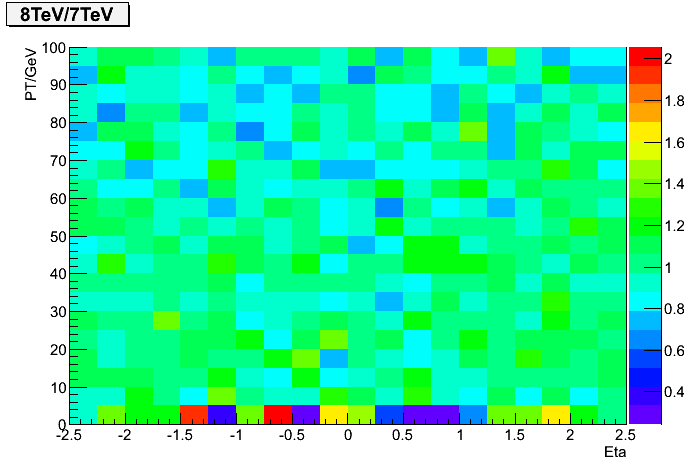
\includegraphics[width=0.55\textwidth]{plots/signal_reweight/ratio_180.png}
%%    \caption{ Ratio of 8TeV/7TeV. }
%%    \label{fig:8TeV7TeVratio}}
%%\end{figure}
%%%higgs
%%\begin{figure}[h!t]
%%  {\centering
%%    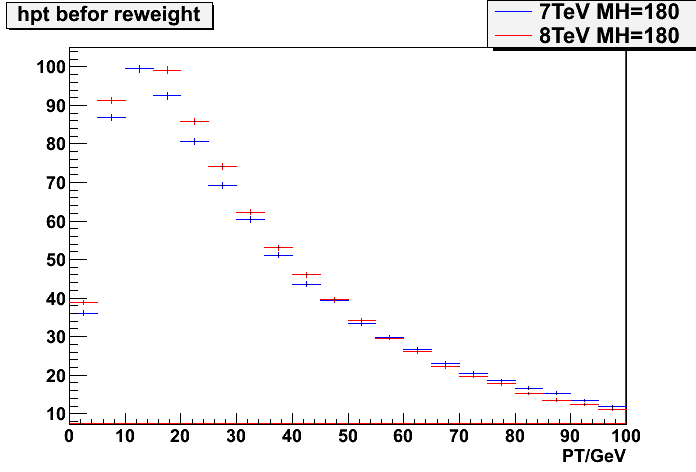
\includegraphics[width=0.49\textwidth]{plots/signal_reweight/Plots/hpt_nw.png}
%%    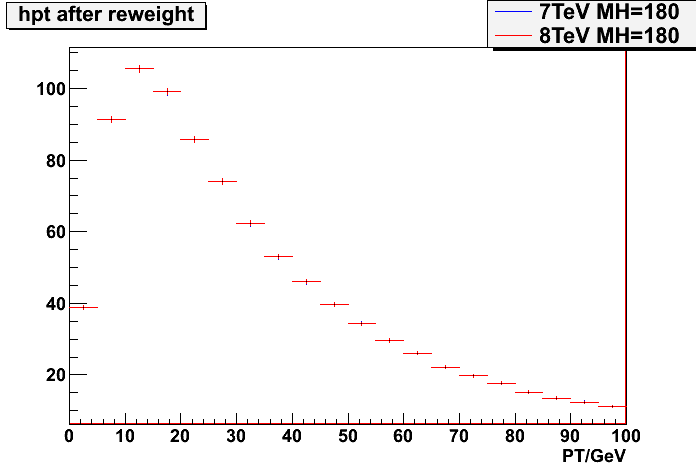
\includegraphics[width=0.49\textwidth]{plots/signal_reweight/Plots/hpt.png}
%%    \caption{Comparison of higgs pt, before and after reweighting.}
%%    \label{fig:higgspt}}
%%\end{figure}
%%\begin{figure}[h!t]
%%  {\centering
%%    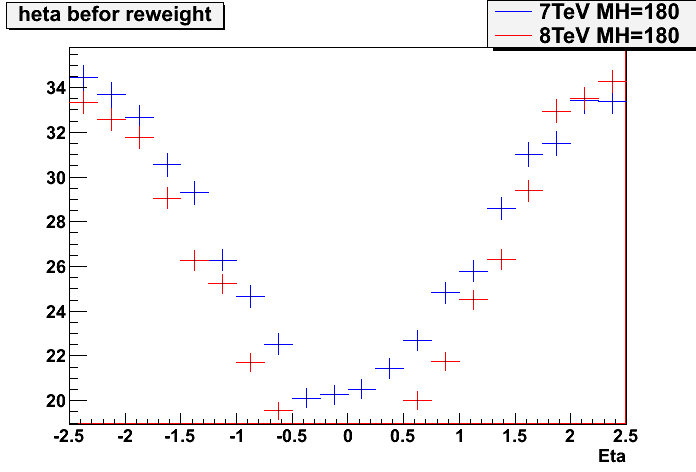
\includegraphics[width=0.49\textwidth]{plots/signal_reweight/Plots/heta_nw.png}
%%    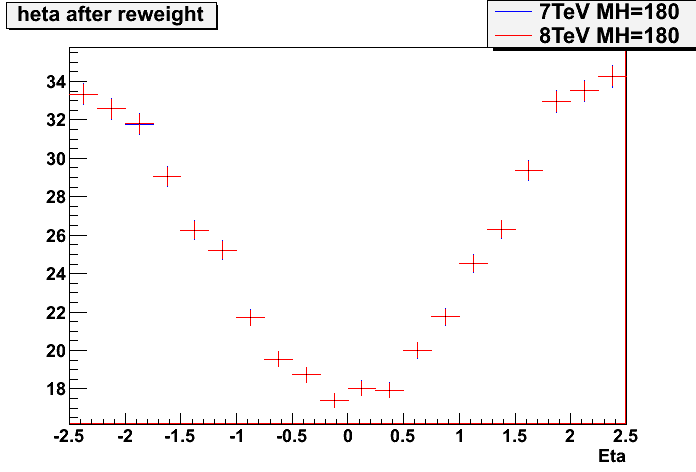
\includegraphics[width=0.49\textwidth]{plots/signal_reweight/Plots/heta.png}
%%    \caption{Comparison of higgs eta, before and after reweighting.}
%%    \label{fig:higgseta}}
%%\end{figure}
%%\begin{figure}[h!t]
%%  {\centering
%%    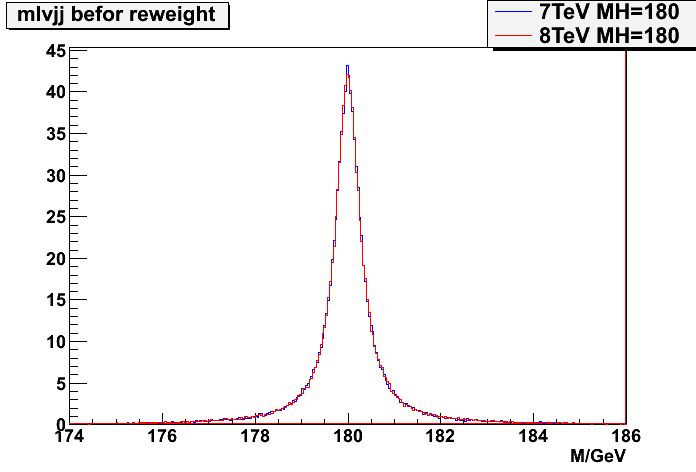
\includegraphics[width=0.49\textwidth]{plots/signal_reweight/Plots/mlvjj_nw.png}
%%    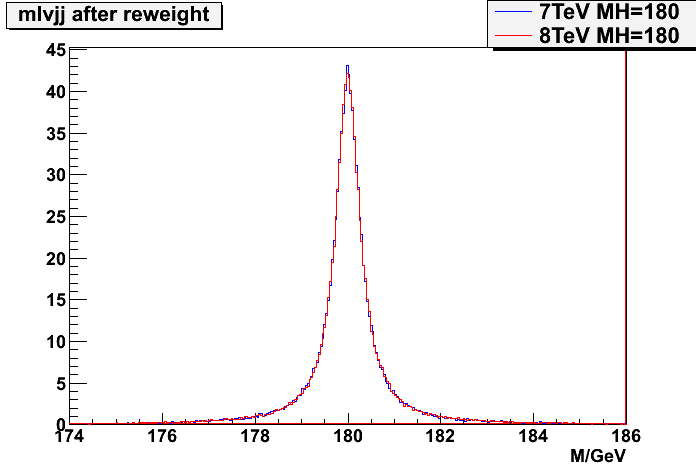
\includegraphics[width=0.49\textwidth]{plots/signal_reweight/Plots/mlvjj.png}
%%    \caption{Comparison of four body mass, before and after reweighting. The lvjj mass was reconstructed by adding the lepton, the nutrino, and the 2 jets decayed by higgs.}
%%    \label{fig:fourbodymass}}
%%\end{figure}
%%
%%%wplus
%%\begin{figure}[h!t]
%%  {\centering
%%    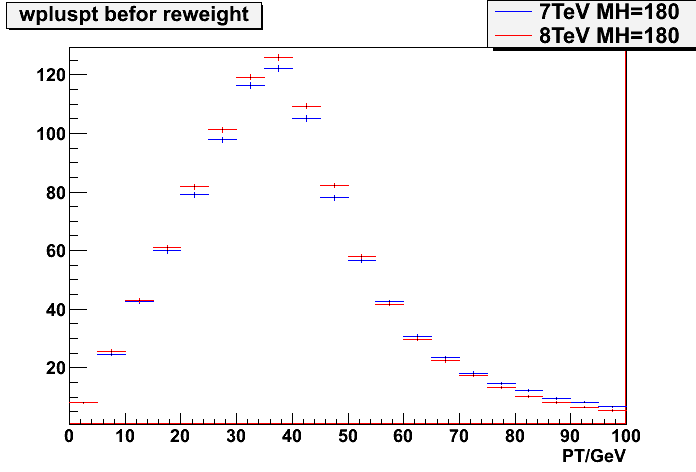
\includegraphics[width=0.49\textwidth]{plots/signal_reweight/Plots/wpluspt_nw.png}
%%    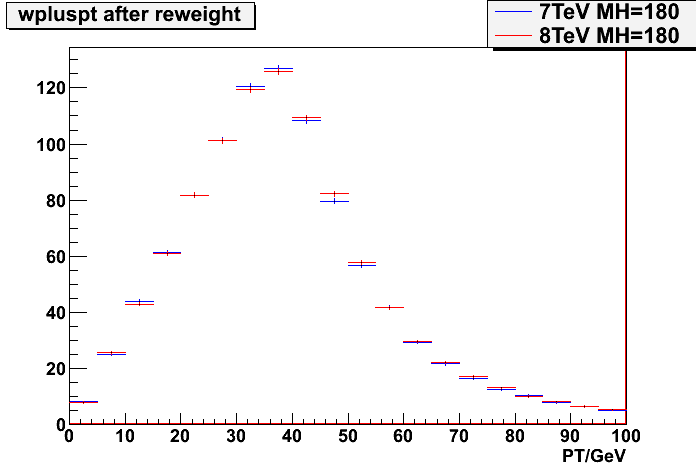
\includegraphics[width=0.49\textwidth]{plots/signal_reweight/Plots/wpluspt.png}
%%    \caption{Comparison of wplus pt, before and after reweighting.}
%%    \label{fig:wpluspt}}
%%\end{figure}
%%\begin{figure}[h!t]
%%  {\centering
%%    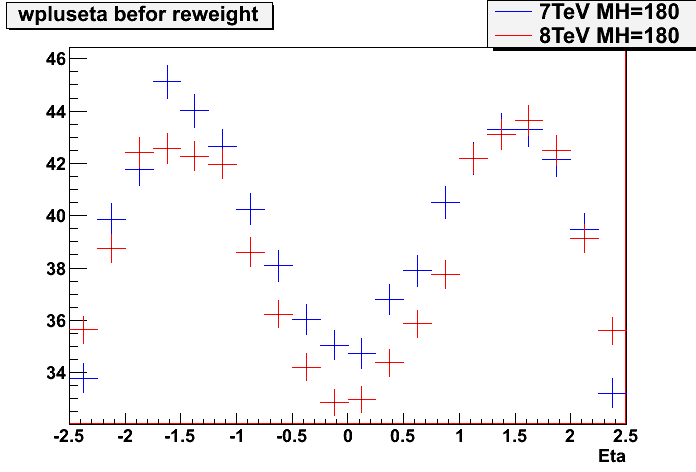
\includegraphics[width=0.49\textwidth]{plots/signal_reweight/Plots/wpluseta_nw.png}
%%    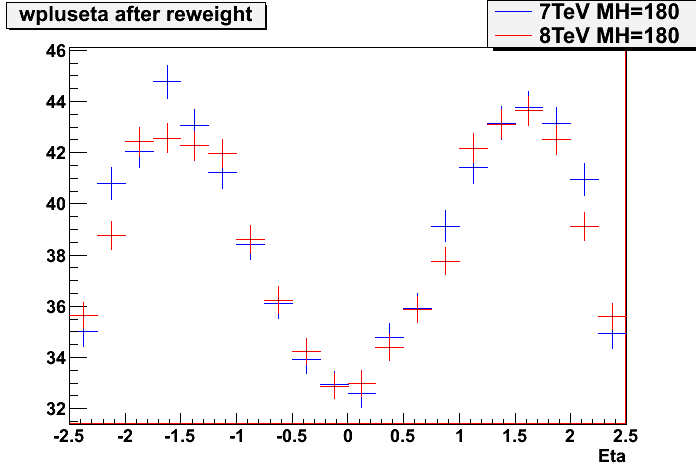
\includegraphics[width=0.49\textwidth]{plots/signal_reweight/Plots/wpluseta.png}
%%    \caption{Comparison of wplus eta, before and after reweighting.}
%%    \label{fig:wpluseta}}
%%\end{figure}
%%%wminus
%%\begin{figure}[h!t]
%%  {\centering
%%    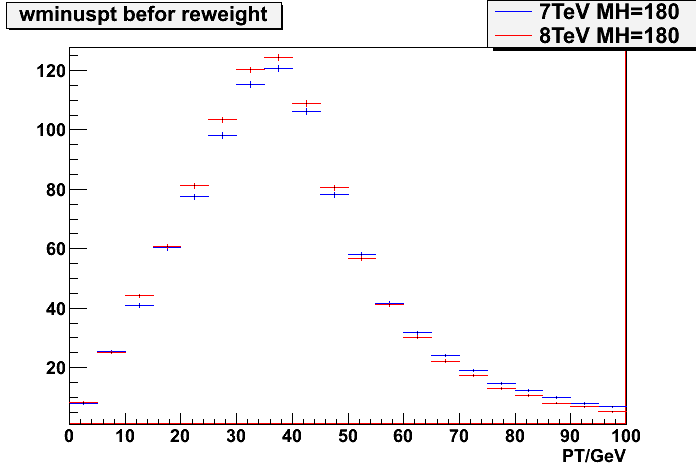
\includegraphics[width=0.49\textwidth]{plots/signal_reweight/Plots/wminuspt_nw.png}
%%    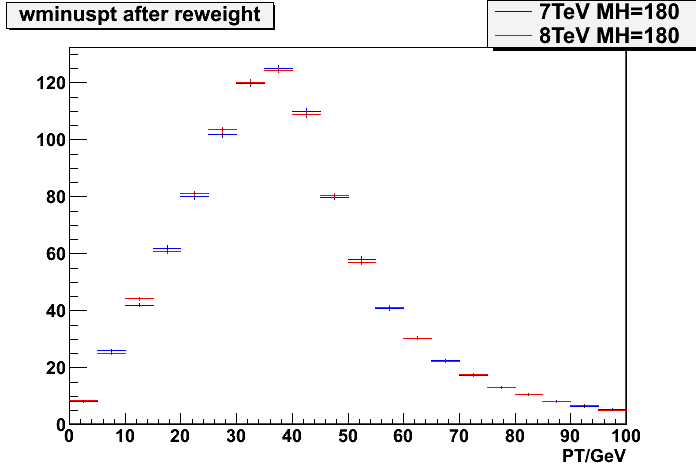
\includegraphics[width=0.49\textwidth]{plots/signal_reweight/Plots/wminuspt.png}
%%    \caption{Comparison of wminus pt, before and after reweighting.}
%%    \label{fig:wminuspt}}
%%\end{figure}
%%\begin{figure}[h!t]
%%  {\centering
%%    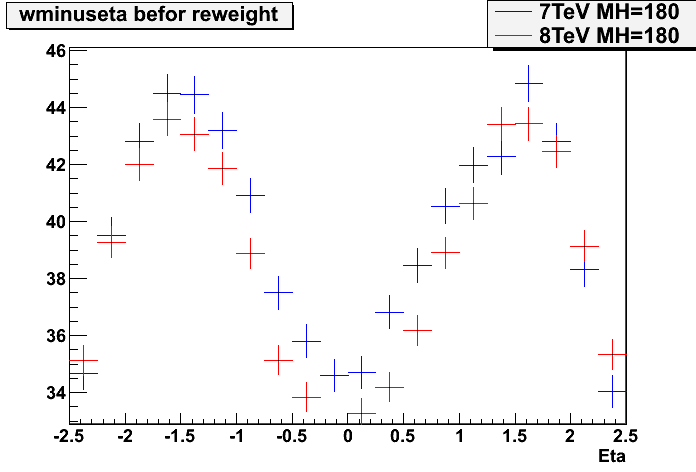
\includegraphics[width=0.49\textwidth]{plots/signal_reweight/Plots/wminuseta_nw.png}
%%    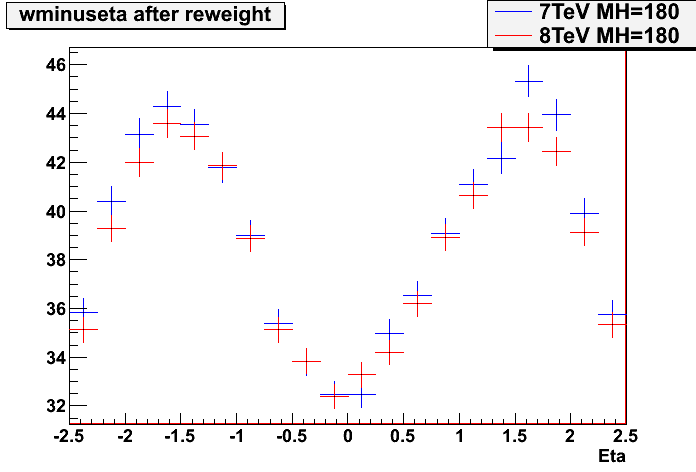
\includegraphics[width=0.49\textwidth]{plots/signal_reweight/Plots/wminuseta.png}
%%    \caption{Comparison of wminus eta, before and after reweighting.}
%%    \label{fig:wminuseta}}
%%\end{figure}
%%
%%%ele
%%\begin{figure}[h!t]
%%  {\centering
%%    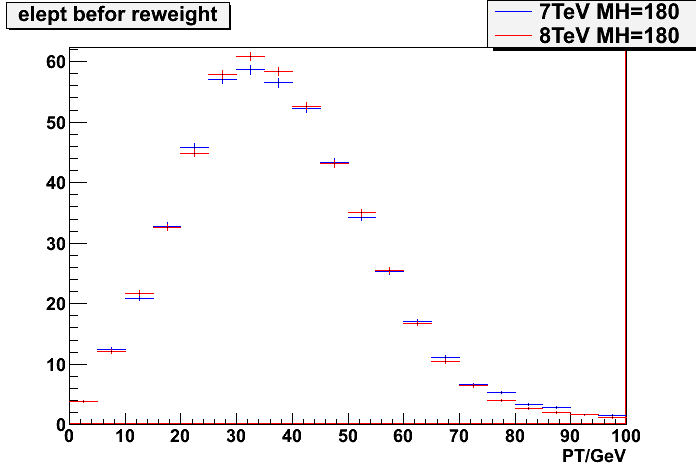
\includegraphics[width=0.49\textwidth]{plots/signal_reweight/Plots/elept_nw.png}
%%    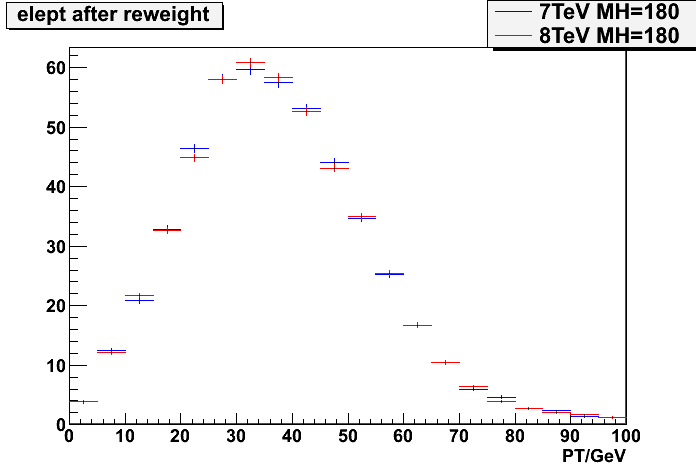
\includegraphics[width=0.49\textwidth]{plots/signal_reweight/Plots/elept.png}
%%    \caption{Comparison of electron pt, before and after reweighting.}
%%    \label{fig:electronpt}}
%%\end{figure}
%%\begin{figure}[h!t]
%%  {\centering
%%    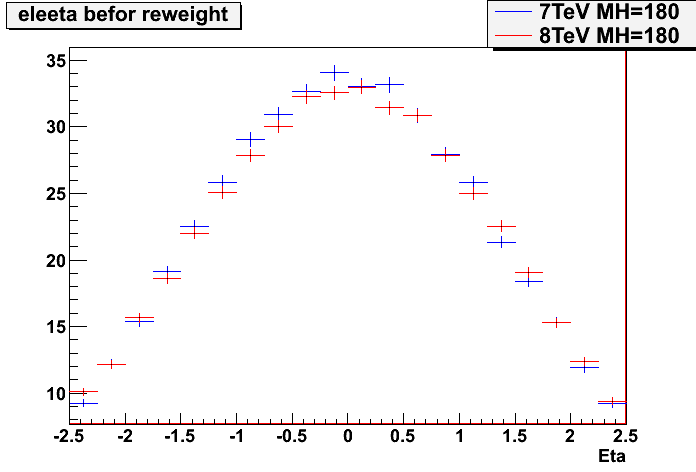
\includegraphics[width=0.49\textwidth]{plots/signal_reweight/Plots/eleeta_nw.png}
%%    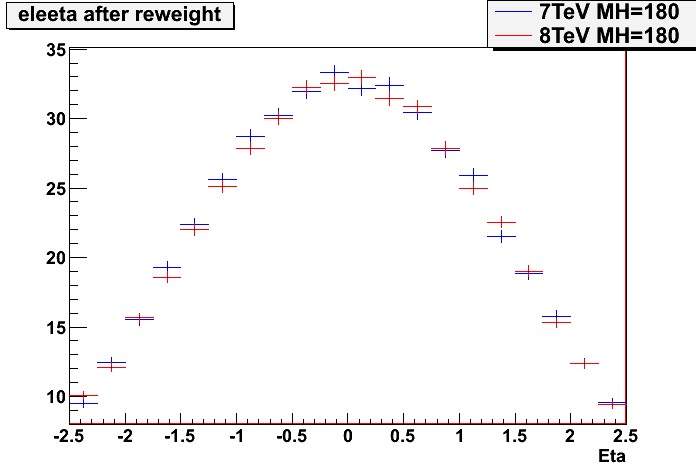
\includegraphics[width=0.49\textwidth]{plots/signal_reweight/Plots/eleeta.png}
%%    \caption{Comparison of elctron eta, before and after reweighting.}
%%    \label{fig:elctroneta}}
%%\end{figure}
%%%mu
%%\begin{figure}[h!t]
%%  {\centering
%%    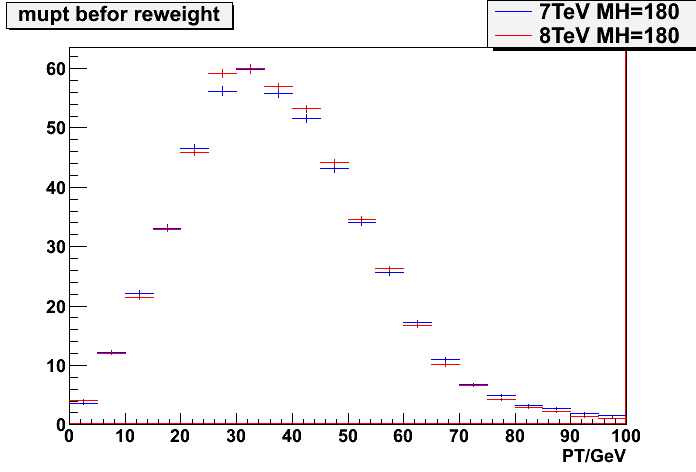
\includegraphics[width=0.49\textwidth]{plots/signal_reweight/Plots/mupt_nw.png}
%%    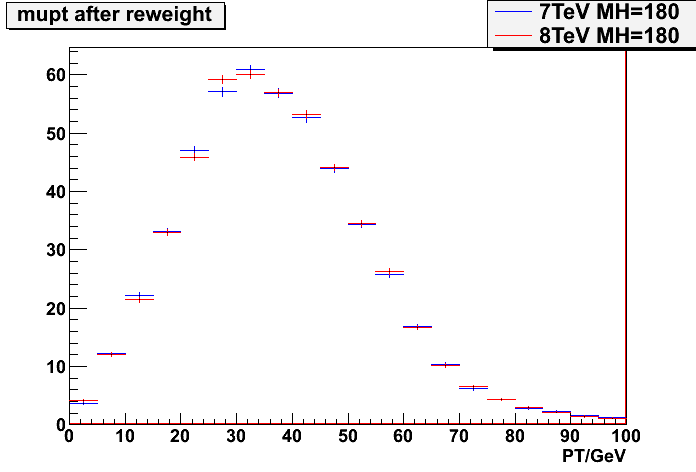
\includegraphics[width=0.49\textwidth]{plots/signal_reweight/Plots/mupt.png}
%%    \caption{Comparison of muon pt, before and after reweighting.}
%%    \label{fig:muonpt}}
%%\end{figure}
%%\begin{figure}[h!t]
%%  {\centering
%%    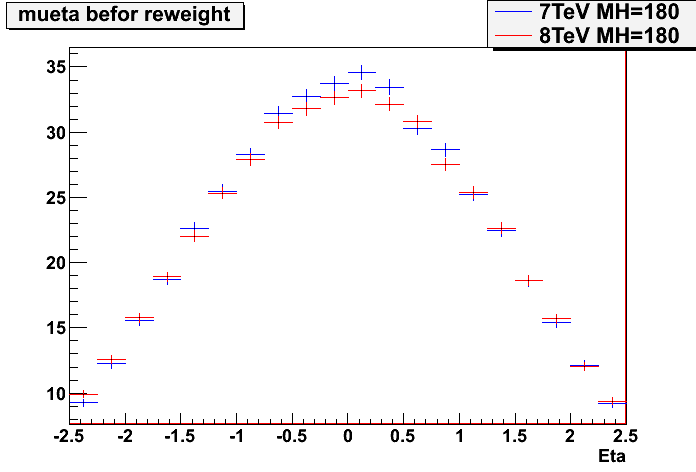
\includegraphics[width=0.49\textwidth]{plots/signal_reweight/Plots/mueta_nw.png}
%%    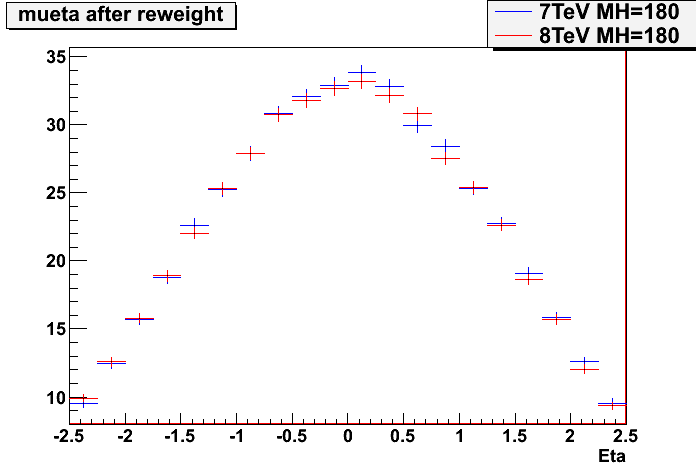
\includegraphics[width=0.49\textwidth]{plots/signal_reweight/Plots/mueta.png}
%%    \caption{Comparison of muon eta, before and after reweighting.}
%%    \label{fig:muoneta}}
%%\end{figure}
%%%jet
%%\begin{figure}[h!t]
%%  {\centering
%%    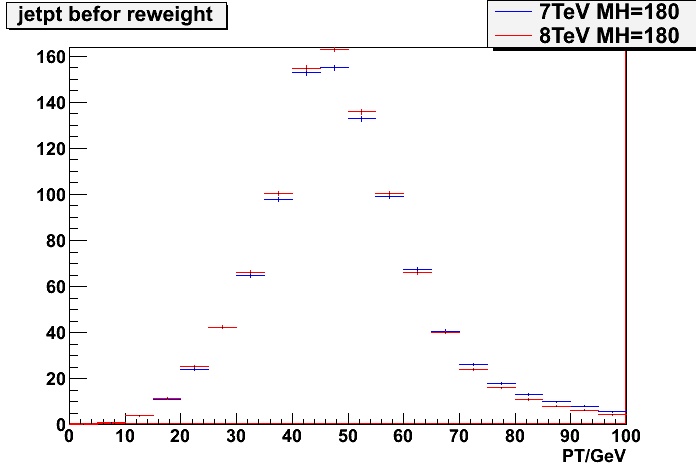
\includegraphics[width=0.49\textwidth]{plots/signal_reweight/Plots/jetpt_nw.png}
%%    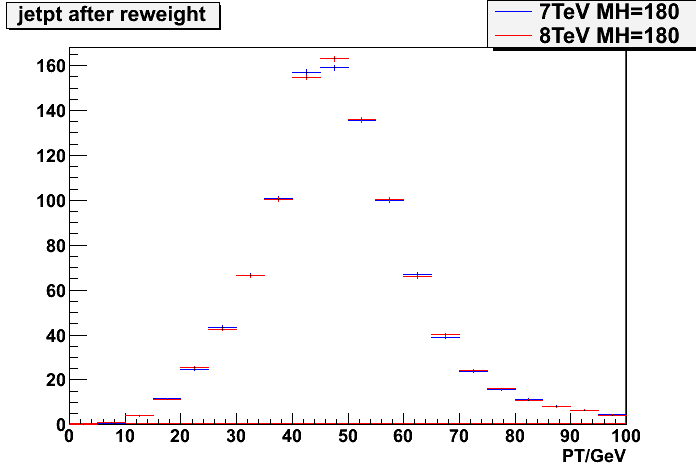
\includegraphics[width=0.49\textwidth]{plots/signal_reweight/Plots/jetpt.png}
%%    \caption{Comparison of leading jet pt, before and after reweighting.}
%%    \label{fig:leadingjetpt}}
%%\end{figure}
%%\begin{figure}[h!t]
%%  {\centering
%%    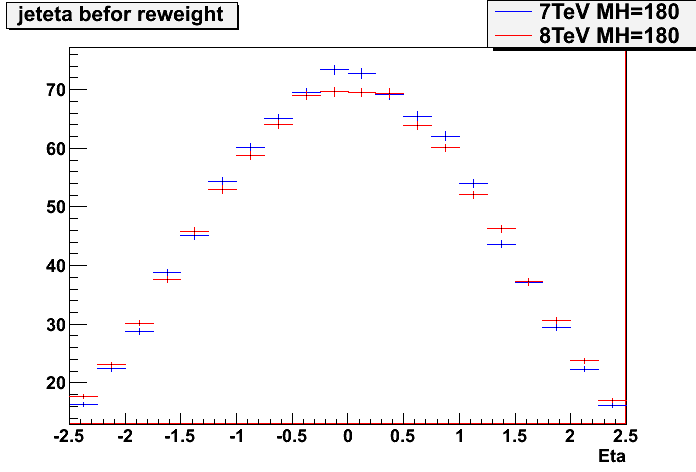
\includegraphics[width=0.49\textwidth]{plots/signal_reweight/Plots/jeteta_nw.png}
%%    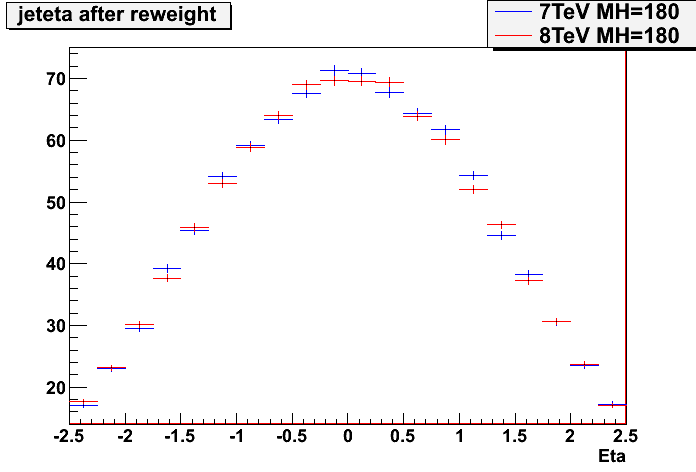
\includegraphics[width=0.49\textwidth]{plots/signal_reweight/Plots/jeteta.png}
%%    \caption{Comparison of leading jet eta, before and after reweighting.}
%%    \label{fig:leadingjeteta}}
%%\end{figure}
%%%nutrino
%%\begin{figure}[h!t]
%%  {\centering
%%    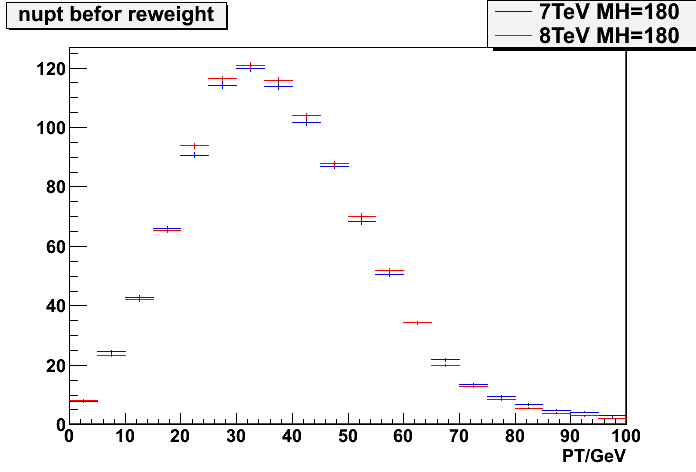
\includegraphics[width=0.49\textwidth]{plots/signal_reweight/Plots/nupt_nw.png}
%%    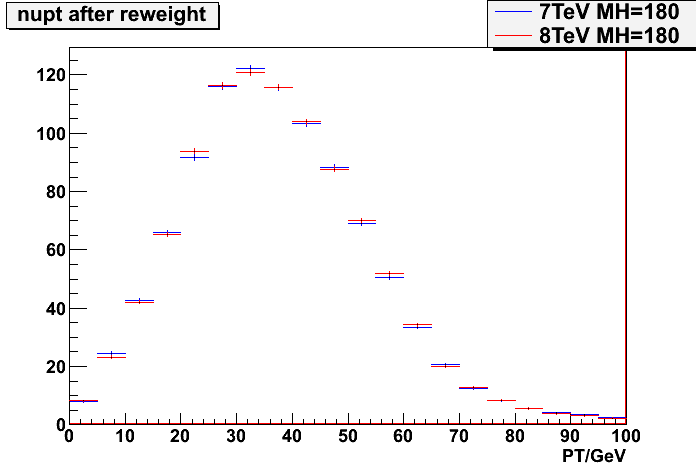
\includegraphics[width=0.49\textwidth]{plots/signal_reweight/Plots/nupt.png}
%%    \caption{Comparison of nutrino pt, before and after reweighting.}
%%    \label{fig:nutrinopt}}
%%\end{figure}
%%
%%%\begin{figure}[h!t]
%%%  {\centering
%%%    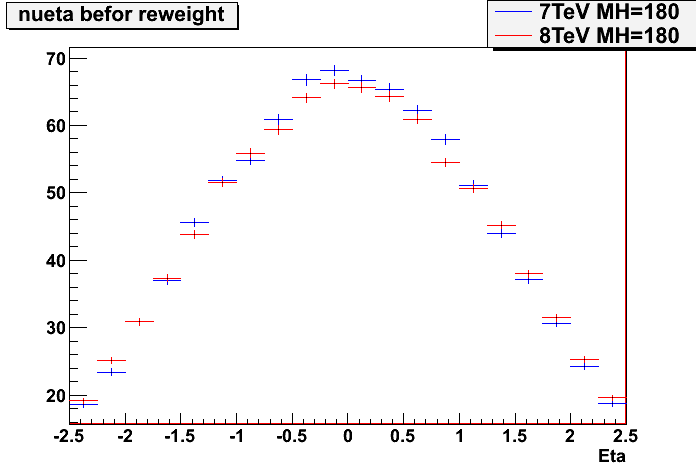
\includegraphics[width=0.49\textwidth]{plots/signal_reweight/Plots/nueta_nw.png}
%%%    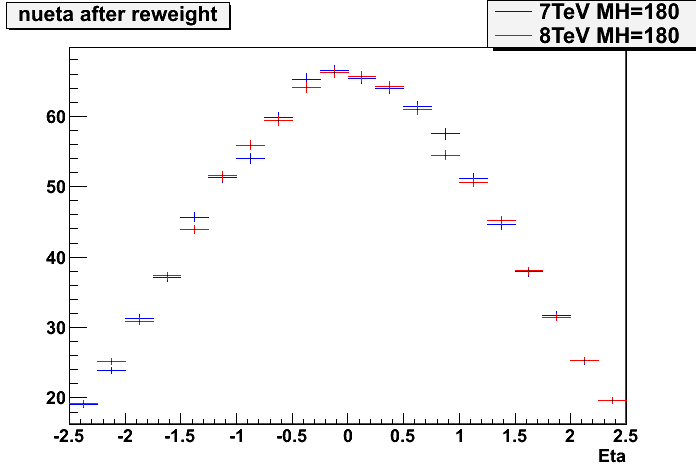
\includegraphics[width=0.49\textwidth]{plots/signal_reweight/Plots/nueta.png}
%%%    \caption{Comparison of nutrino eta, before and after reweighting.}
%%%    \label{fig:nutrino eta}}
%%%\end{figure}


\clearpage
      % what samples and triggers have been used  
\section{Common Event Selection}
\label{sec:firstStep}
% ---- ---- ---- ---- ---- ---- ---- ---- ---- ---- ---- ---- ---- ---- ---- ---- ---- ---- ---- ---- ---- ---- ----

The final state of the Higgs decay is characterized by a charged lepton, 
large missing energy and two hadronic jets that form a W.
In this section we first describe the criteria applied to objects
selected in the event and then we describe the requirements made at
the event-level.

\subsection{Object Definitions}

The analysis relies on the standard reconstruction algorithms produced
by the CMS community. 
The PF2PAT procedure was used to coherently define the collection of particle-flow jets, leptons and
MET considered in the event selection.  
The technical details of the software configuration can be found in the group twiki page~\cite{WG_PATtuple_twiki}. 

\subsubsection{Electron Cuts (e+jets)}
\label{sec:electron_cuts}

Electrons are reconstructed using a gaussian sum 
filter (GSF) algorithm \cite{CMS-PAS-EGM-10-004},
and are required to pass electron ID cuts according 
to the simple cut-based electron ID~\cite{simplecutbasedelectronid}, 
with the ``VBTF Working Point 70''. 
The GSF algorithm accounts for possible energy loss due to
bremsstrahlung in the tracker layers.
The energy of an electron candidate with $\et>35~\gev$ is essentially
determined by the ECAL cluster energy, while its momentum direction
is determined by that of the associated track.
The simple cut based electron ID relies on three shower
shape variables with different cut values for the barrel and
the endcap regions, as shown in Table~\ref{tab:EleID}.

Additionally, we require
%%%%%%%%%%%%%%%%%%%
\begin{itemize}
\item Electron $E_\mathrm{T} > 35\,\mathrm{GeV}$.
\item Pseudorapidity $|\eta| < 2.5$. There is an exclusion range due
        to the ECAL barrel-endcap transition region, defined by
        $1.4442 < |\eta_{\mathrm{sc}}| < 1.566$, where
        $\eta_{\mathrm{sc}}$ is the pseudorapidity of the ECAL
        supercluster.
\item Impact parameter: We cut on the absolute value of the impact
       parameter calculated with respect to the average beamspot. We
       require:  $d_0(\mathrm{Bsp}) < 0.02\,\mathrm{cm}.$   
\item The selected electron candidates have to be isolated simultaneously in
the tracker, and in the electromagnetic and hadronic calorimeters.  Combined
relative isolation is defined as
%%%
\begin{equation*}
\mathrm{RelIso_{\mathrm{Comb}}} = \frac{I_{\mathrm{Trk}}+I_{\mathrm{EM}}+I_{\mathrm{had}}}{E_\mathrm{T}}.
\end{equation*} 
%%%
The electron candidate is required to have 
$\mathrm{RelIso_{\mathrm{Comb}}} < 0.05$ in order 
to be considered isolated. 
A pile-up offset subtraction in the isolation cone 
using fastjet algorithm \cite{FastJetPUSubtraction} is applied.
We also veto the presence of a second loose lepton in the event.
\item 
In order to reject events in which the electron candidate actually
originates from a conversion of a photon into an $e^{+}e^{-}$ pair, we
require the number of missed inner tracker layers of the electron
track to be exactly zero (i.e. there are no missed layers before the
first hit of the electron track from the beam line). In addition, we
reject any event in which the selected electron is flagged as a
conversion, \textit{i.e.}, an electron that has a 
distance of the partner track $|$\texttt{dist}$|$ $< 0.02$~mm and an
opening angle $|$\texttt{dcot}$|$ $< 0.02$~\cite{ConversionRejection}.
\end{itemize}
%%%%%%%%%%%%%%%%%%%
%%%%%%%%%%%%%%%%%%%
%%%%%%%%%%%%%%%%%%%
\begin{table}[bthp]
\begin{center}
{\footnotesize
\begin{tabular}{|c|c|c|c|c|}
\hline
ID Variable & WP70 Barrel & WP70 Endcaps & WP95 Barrel & WP95 Endcaps  \\
\hline
$\sigma_{i\eta i\eta}$ & 0.01 & 0.03 & 0.01 & 0.03 \\
$\phi_{\mathrm{SC}} - \phi_{\mathrm{trk}}$ & 0.03 & 0.02 & 0.8 & 0.7 \\
$\eta_{\mathrm{SC}} - \eta_{\mathrm{trk}}$ & 0.004 & 0.005 & 0.007 & 0.01 \\
\hline
\end{tabular}
\caption[.]{\label{tab:EleID} Cut values for electron identification
variables for VBTF Working Point (WP) 70 (barrel and endcap), as used
for the tight electron selection, and VBTF Working Point (WP) 95
(barrel and endcap), as used in the loose electron selection.}}
\end{center}
\end{table}
%%%%%%%%%%%%%%%%%%%
%%%%%%%%%%%%%%%%%%%%%%%%%%%%%%%%%%%%%%%%%%%%%%%%%%%%%%%%%%%%%%%%%%%%%%%%%%%%
%%%%%%%%%%%%%%%%%%%%%%%%%%%%%%%%%%%%%%%%%%%%%%%%%%%%%%%%%%%%%%%%%%%%%%%%%%%%

\subsubsection{Muon Cuts (mu+jets)}
\label{sec:muon_cuts}

Muon candidates are identified by two different 
algorithms~\cite{MUONPAS}: one proceeds from the inner tracker outwards, 
the other one starts from tracks measured in the muon chambers and matches 
and combines them with tracks reconstructed in the inner tracker. 
These selection criteria are summarized below:
%%%%%%%%%%%%%%%%%%%
\begin{itemize}
\item The muon candidate is reconstructed both as a global muon and
as a tracker muon.
\item The number of hits of the muon track in the silicon tracker has
to be $N_{\mathrm{Hits}} > 10$.
\item Number of pixel hits of the Tracker track $\ge 1$;
\item Number of muon hits of the Global track $\ge 2$;
\item Normalized $\chi^{2}$ of the Global track $< 10.0$.
\item Muon $p_{\mathrm{T}} > 25\,\mathrm{GeV}$.
\item Pseudorapidity $|\eta| < 2.1$.
\item Impact parameter: We cut on the absolute value of the impact
parameter calculated with respect to the beamspot. We require:
$d_0(\mathrm{Bsp}) < 0.02\,\mathrm{cm}.$
\item In order to make sure that the selected muon and the selected
jets come from the same hard interaction and not from pile up events,
we require that the $z$ coordinate of the PV of the event and the $z$
coordinate of the muon's inner track vertex lie within a distance of
less than 1~cm.
\item The selected muon candidates also have to be isolated.
We require the muon to be isolated simultaneously in the
tracker, and in the electromagnetic and hadronic calorimeters.  
The muon candidate is required to have
$\mathrm{RelIso_{\mathrm{Comb}}} < 0.1$ in order to be considered
isolated.
We also veto the presence of a second loose lepton in the event.
\end{itemize}

%%%%%%%%%%%%%%%%%%%%%%%%%%%%
%%%%%%%%%%%%%%%%%%%%%%%%%%%%
%%%%%%%%%%%%%%%%%%%%%%%%%%%%%%%%%%%%%%%%%%%%%%%%%%%%%%%%%%%%%%%%%%%%%%%%%%%%
%%%%%%%%%%%%%%%%%%%%%%%%%%%%%%%%%%%%%%%%%%%%%%%%%%%%%%%%%%%%%%%%%%%%%%%%%%%%


\subsubsection{Loose Electron}
For the purposes of rejecting events with more than one lepton we
define a loose electron, which has looser cuts. We consider electrons
which have $p_{\mathrm{T}} > 15\,\mathrm{GeV}/c$, $|\eta| < 2.5$, and
$\mathrm{RelIso_{\mathrm{Trk}}} < 0.2$ and which satisfy electron ID
cuts according to ``VBTF Working Point 95'' to be ``loose''. The cut
values for the electron ID variables used in the analysis can be found
in table~\ref{tab:EleID}.

\subsubsection{Loose Muon}
Additionally, to reject events with more than one lepton, we define a
loose muon, which has looser cuts. We consider all global muons which
have $p_{\mathrm{T}} > 10\,\mathrm{GeV}/c$, $|\eta| < 2.5$, and
$\mathrm{RelIso_{\mathrm{Trk}}} < 0.2$ to be loose muons.

\subsubsection{Jet Cuts}
\label{sec:firstStep_jets}

Jets are reconstructed with the anti-KT algorithm \cite{cacciari}, 
starting from the set of objects reconstructed by the particle 
flow \cite{pflow,CMS-PAS-JME-10-003,CMS-PAS-PFT-10-002}.
Jets are corrected such that the measured energy of the jet 
correctly reproduces the energy of the initial particle. 
The CMS standard L2 (relative) correction makes the jet response flat in $\eta$.
The standard L3 (absolute) correction brings the jet closer to the $\PT$ of 
a matched generated jet created using generator level input and a similar 
jet clustering algorithm.
The L2 and L3 corrections are calculated using Monte Carlo, and thus a 
L2L3 residual correction is applied that fixes the discrepancies between 
Monte Carlo and data~\cite{newjes-cms}.
In this analysis we use jets with measured (corrected) $\PT$  
greater than 30~$\gev$. 
We require $|\eta| < 2.4$ so that the jets fall within the
tracker acceptance.  
Jets are required to pass a set of loose identification
criteria; this requirement eliminates jets originating from or being seeded by
noisy channels in the calorimeter~\cite{Chatrchyan:2009hy}: 
%%%%%%%%%%%%%%
\begin{itemize}
\item Fraction of energy due to neutral hadrons $<$ 0.99.
\item Fraction of energy due to neutral EM deposits $<$ 0.99.
\item Number of constituents $>$ 1.
\item Number of charged hadrons candidates $>$ 0.
\item Fraction of energy due to charged hadrons candidates $>$ 0.
\item Fraction of energy due to charged EM deposits $<$ 0.99.
\end{itemize}
%%%%%%%%%%
All energy fractions are calculated from uncorrected jets.

\par
In order to account for electron and muon objects that
have been reconstructed as jets, we remove from the jet
collection any jet that falls within a
cone of radius $R= 0.3$ of a loose electron or a loose muon. 
This ``cleaning'' procedure is applied in order to ensure that the same
particle is not double counted as two different physics objects.
We require exactly two or three jets in the event.


\subsection{Event-Level Criteria}

The event should have a good primary vertex (PV). This means selecting
the primary vertex with the highest sum of $p_{T}^2$ of the tracks
associated with it and requiring it to have a number of degrees of
freedom (ndof) $\ge 4$, where ndof corresponds to the weighted sum of
the number of tracks usd for the construction of the PV. In addition,
the PV must lie in the central detector region of $abs(z) \le
24~\cm{rm}$ and $\rho \le 2~\rm{cm}$ around the nominal interaction
point.

In the e+jets channel, we select events which contain exactly one
tight electron candidate fulfilling the criteria described in
Section~\ref{sec:electron_cuts} and reject events which contain a
loose electron in addition to the tight electron. In this channel we
are only interested in the decay to electron and jets, and we
therefore reject events containing a loose muon.

In the mu+jets channel, we select events which contain exactly one
tight muon candidate whose criteria are described in
Section~\ref{sec:muon_cuts} and reject events which contain an
additional loose muon. In an analoguous way to the e+jets channel, we
reject events containing a loose electron.

In both channels we require an event to have missing transverse energy
(MET) in excess of $30(25)\,\mathrm{GeV}$ in the electron (muon)
channel and to have a $W$ transverse mass of $50\,\mathrm{GeV}$.
These cuts are designed to reduce the background from QCD multijet
production.

We further require exactly two or three jets passing the cuts
described in Section~\ref{sec:firstStep_jets}.  
% We require the
% invariant mass of the dijet system formed by the two highest $p_{T}$
% jets in the event to be between $65$ and $95\,\mathrm{GeV}$.

           % to be revised
\section{Data - Monte Carlo comparisons}
\label{sec:dataMCcomparisons}
% ---- ---- ---- ---- ---- ---- ---- ---- ---- ---- ---- ---- ---- ---- ---- ---- ---- ---- ---- ---- ---- ---- ----

To assess the quality of the modeling provided by the MC simulation we
make comparisons between the MC shape, normalized to the number of
collected events in data, for the background compared to the overall
data yield after applying the event selection criteria.  We show the
distributions of various kinematic variables after applying all the
selection cuts in Figures ~\ref{fig:mu_jet_pt}-\ref{fig:mu_mjj} for
the muon+jets sample and in Figures
~\ref{fig:elec_jet_pt}-\ref{fig:elec_mjj} for the electron+jets
sample.  Eventually, Figure~\ref{fig:lep_mlvjj} shows the four-body
invariant mass, for electrons (on the left) and muons (on the right).
The MC has been been corrected for lepton reconstruction efficiency
and the trigger efficiency.  Besides the kinematics of the single
objects, we show here also the variables that are used in the MVA
discriminant that maximizes the signal-over-background ratio.  Seeing
reasonable agreement gives us confidence in the qualitative aspects of
the MC modeling.
%%%%%%%%%%%%%%%%%%%%%%%%%%%%
\begin{figure}[ht]
  {\centering
    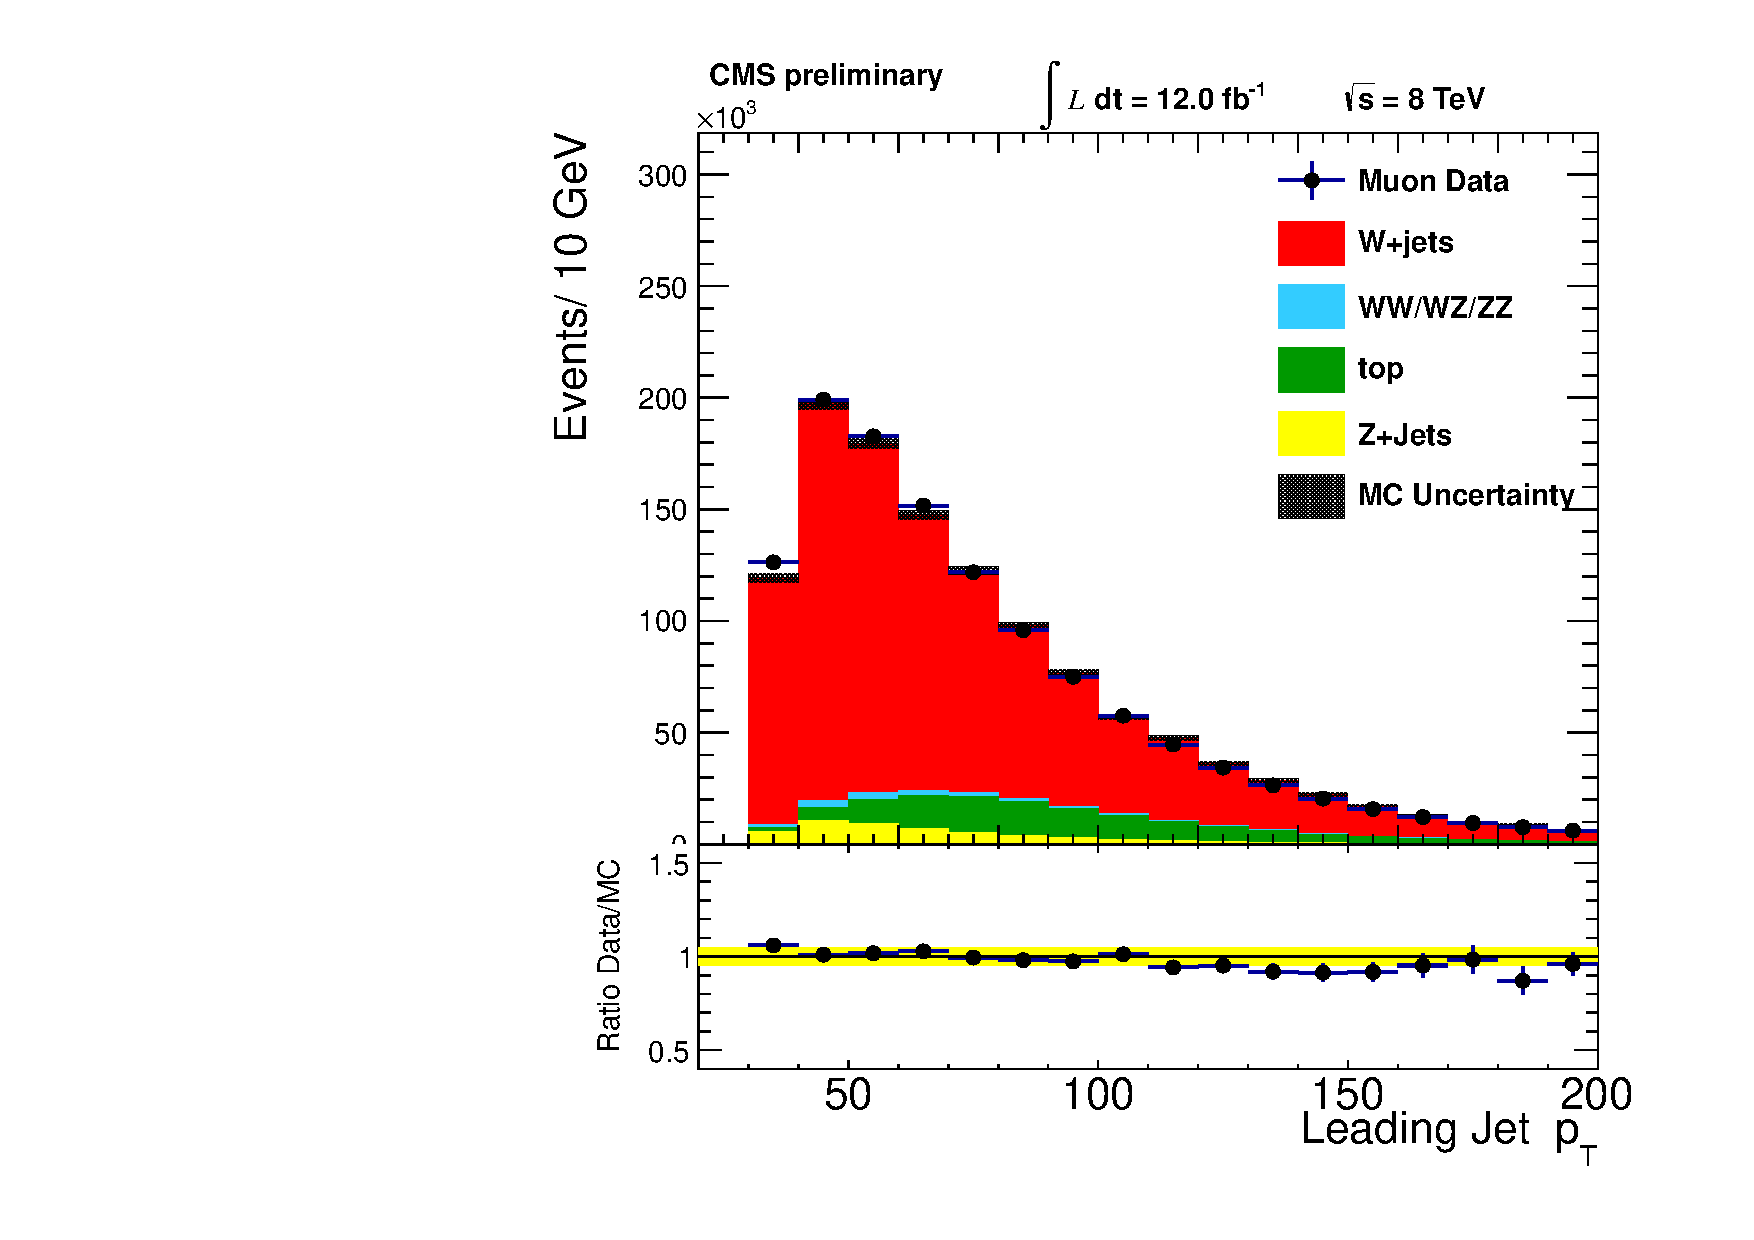
\includegraphics[width=0.49\textwidth]{plots/2012_DataMC/mu_jetld_pt.pdf}
    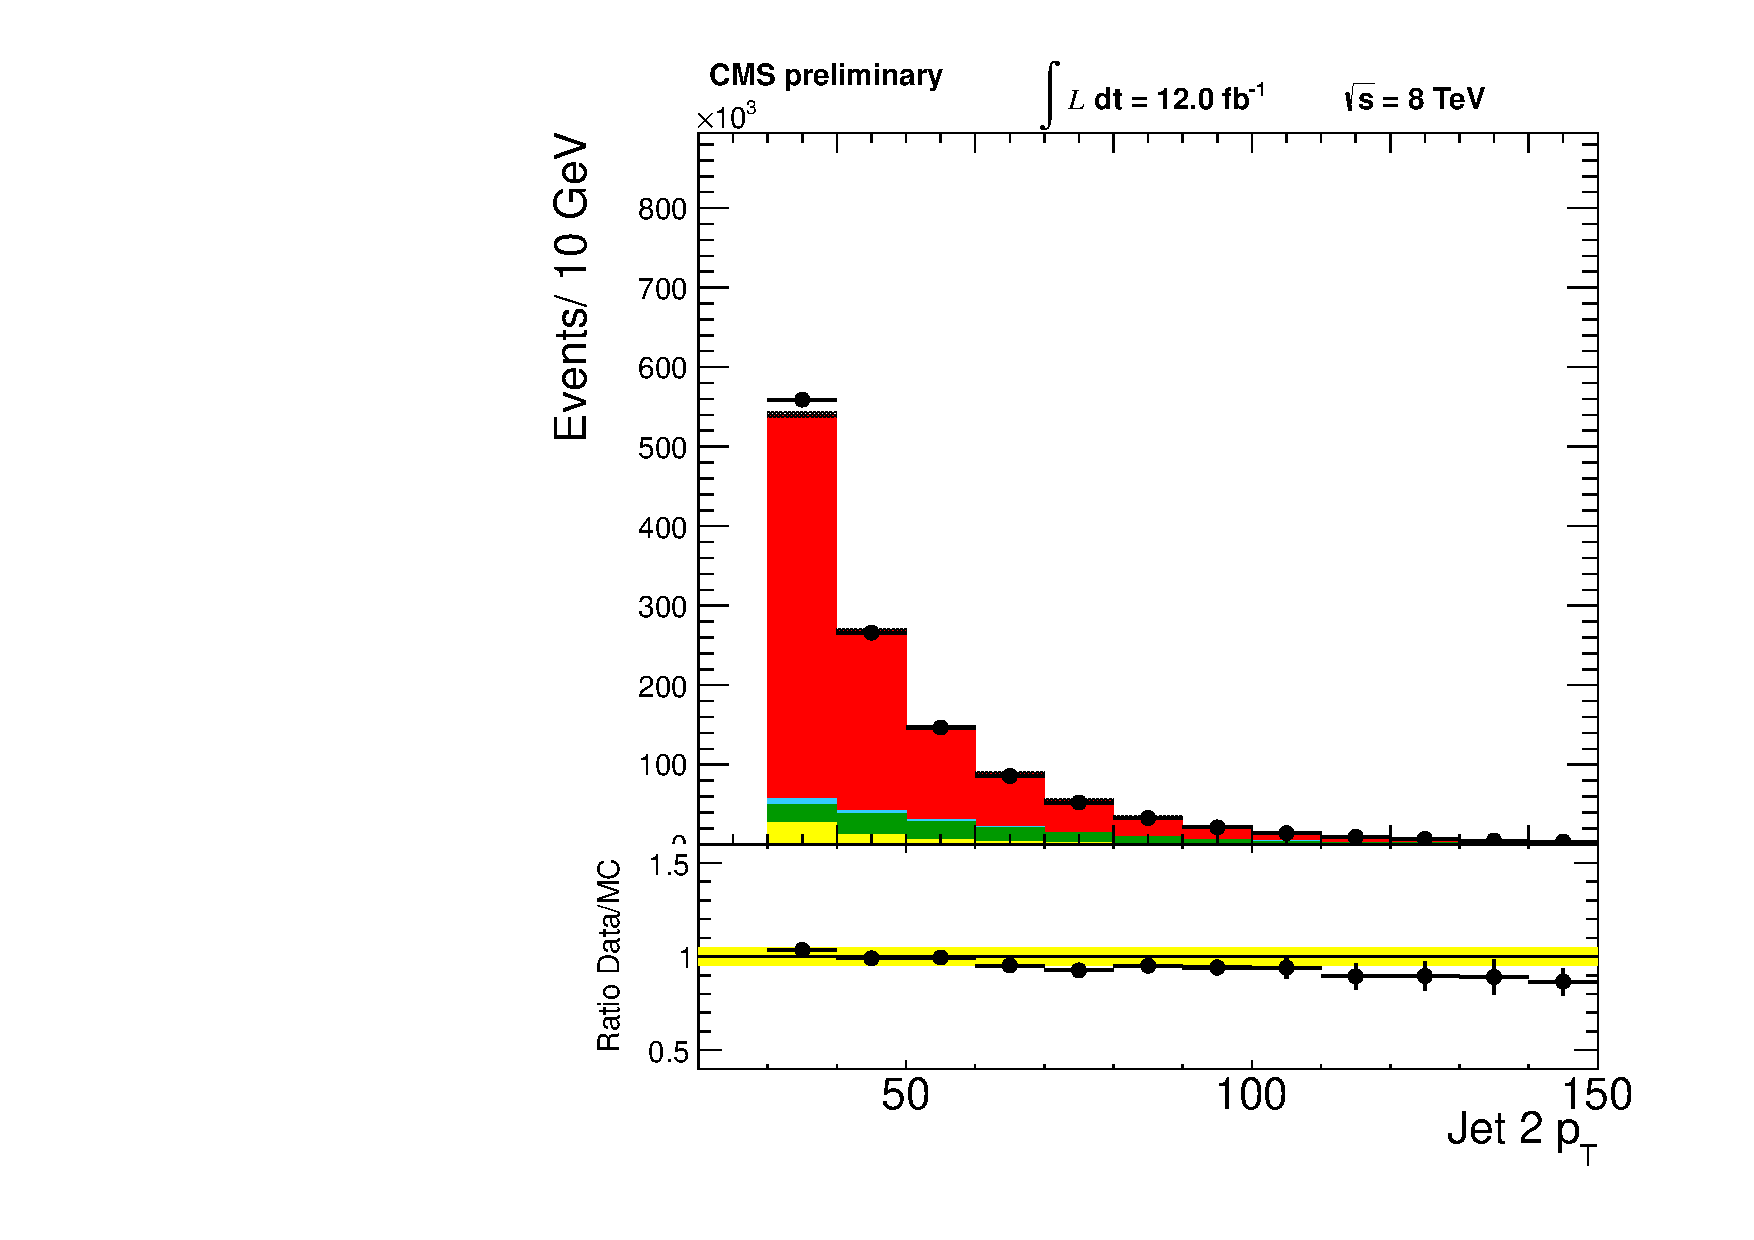
\includegraphics[width=0.49\textwidth]{plots/2012_DataMC/mu_jetnt_pt.pdf}
    \caption{Comparison of the leading jet (left) and 
      the second jet (right) $p_{T}$ distributions from data and MC for the muon+jets
      selection.}
    \label{fig:mu_jet_pt}}
\end{figure}
%%%%%%%%%%%%%%%%%%%%%%%%%%%%
\begin{figure}[h!t]
  {\centering
    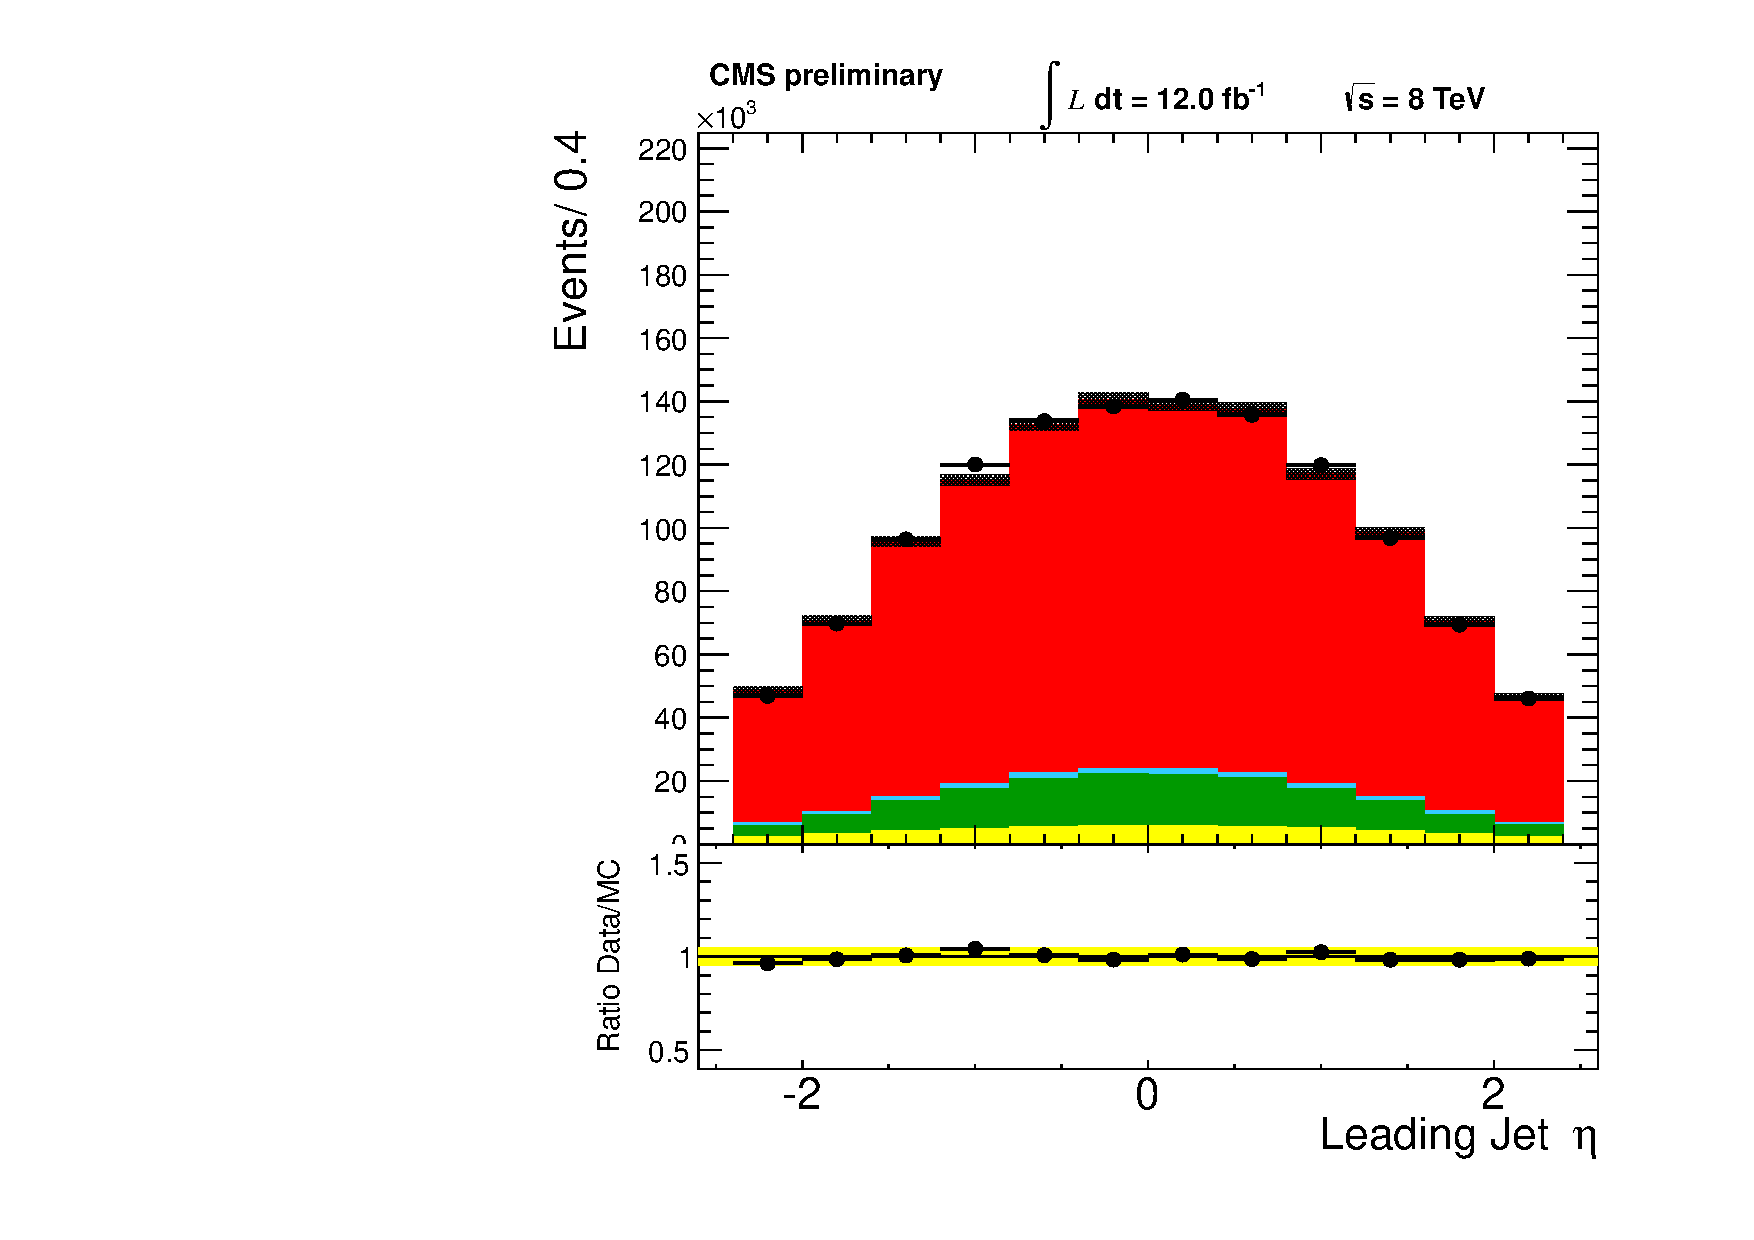
\includegraphics[width=0.49\textwidth]{plots/2012_DataMC/mu_jetld_eta.pdf}
    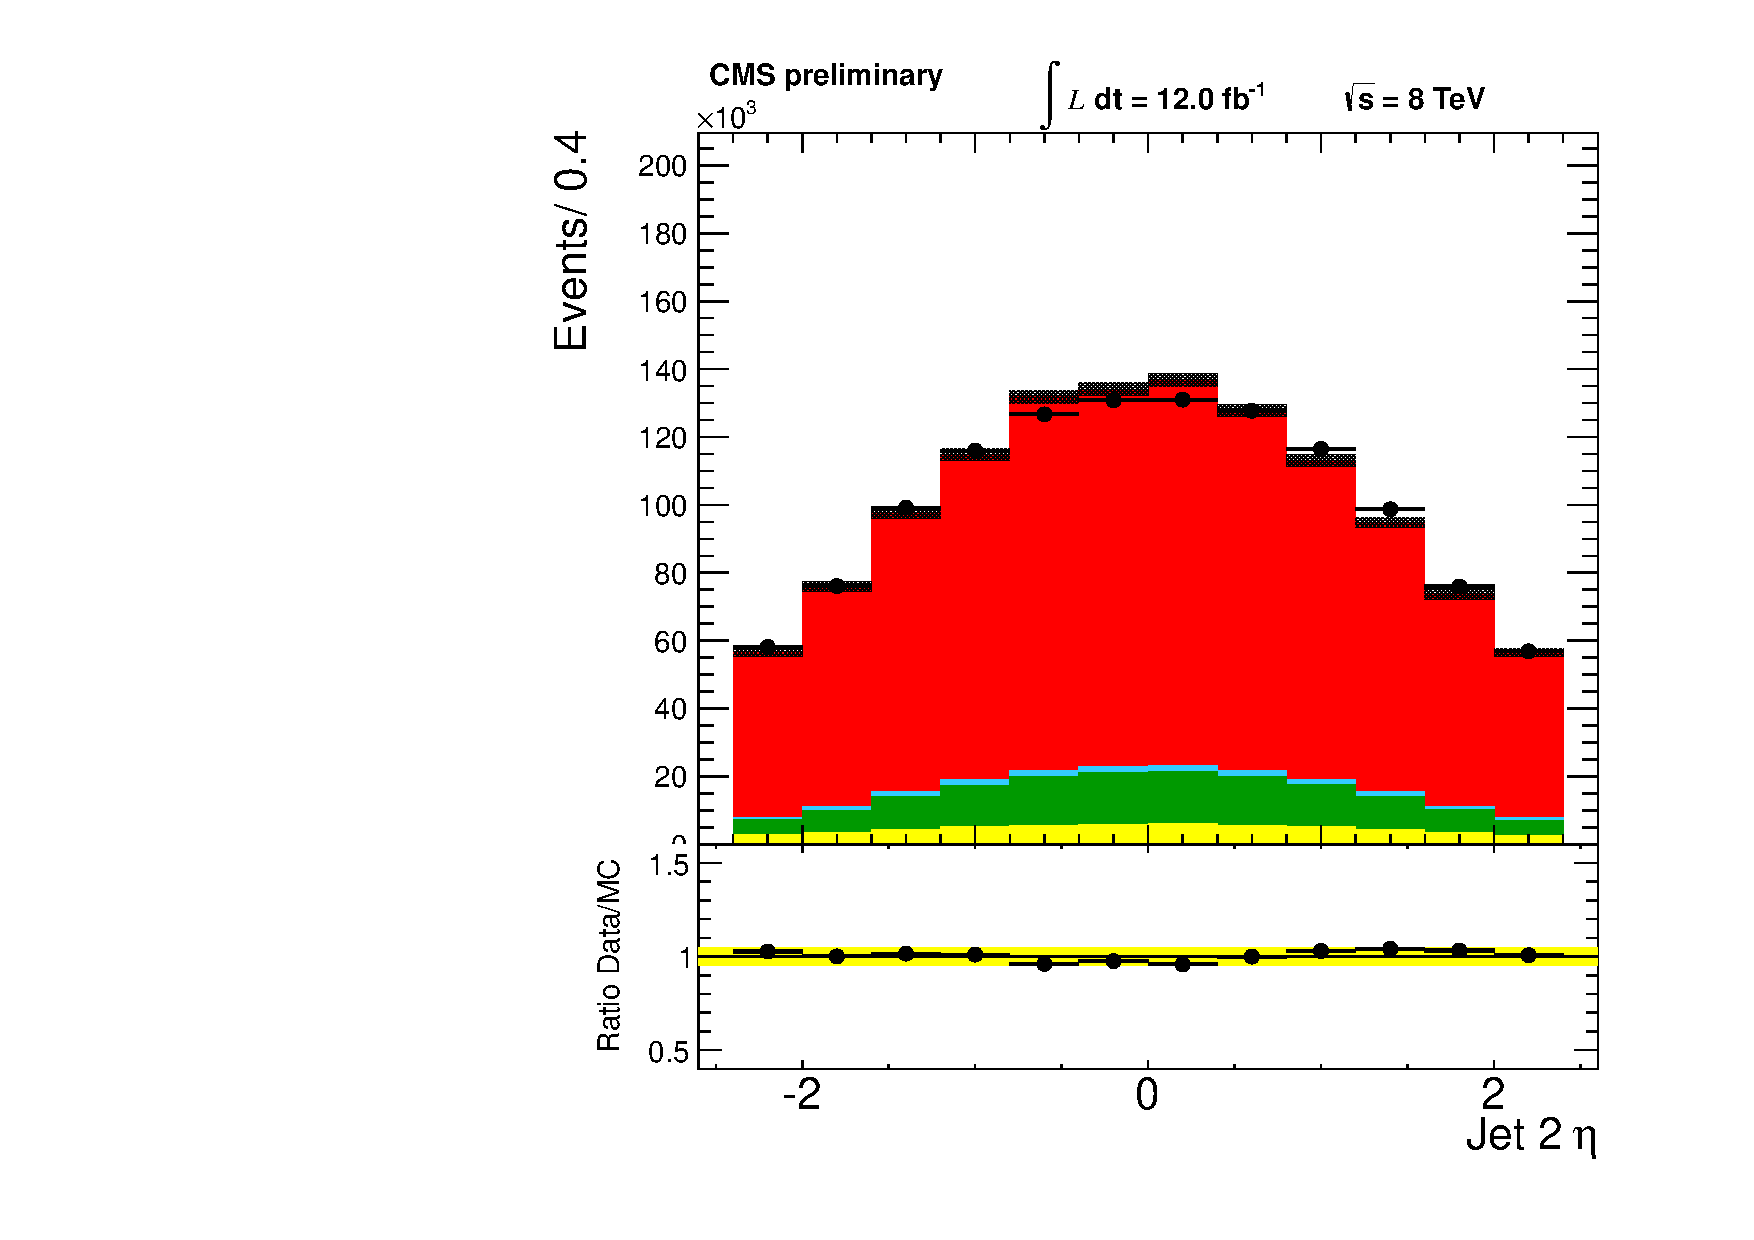
\includegraphics[width=0.49\textwidth]{plots/2012_DataMC/mu_jetnt_eta.pdf}
    \caption{Comparison of the leading jet $\eta $ (left) and the
    second leading jet $\eta $ (right) distributions from data and MC
    for the muon+jets selection.  }
\label{fig:mu_jet_eta}}
\end{figure}
%%%%%%%%%%%%%%%%%%%%%%%%%%%%
\begin{figure}[h!t]
  {\centering
    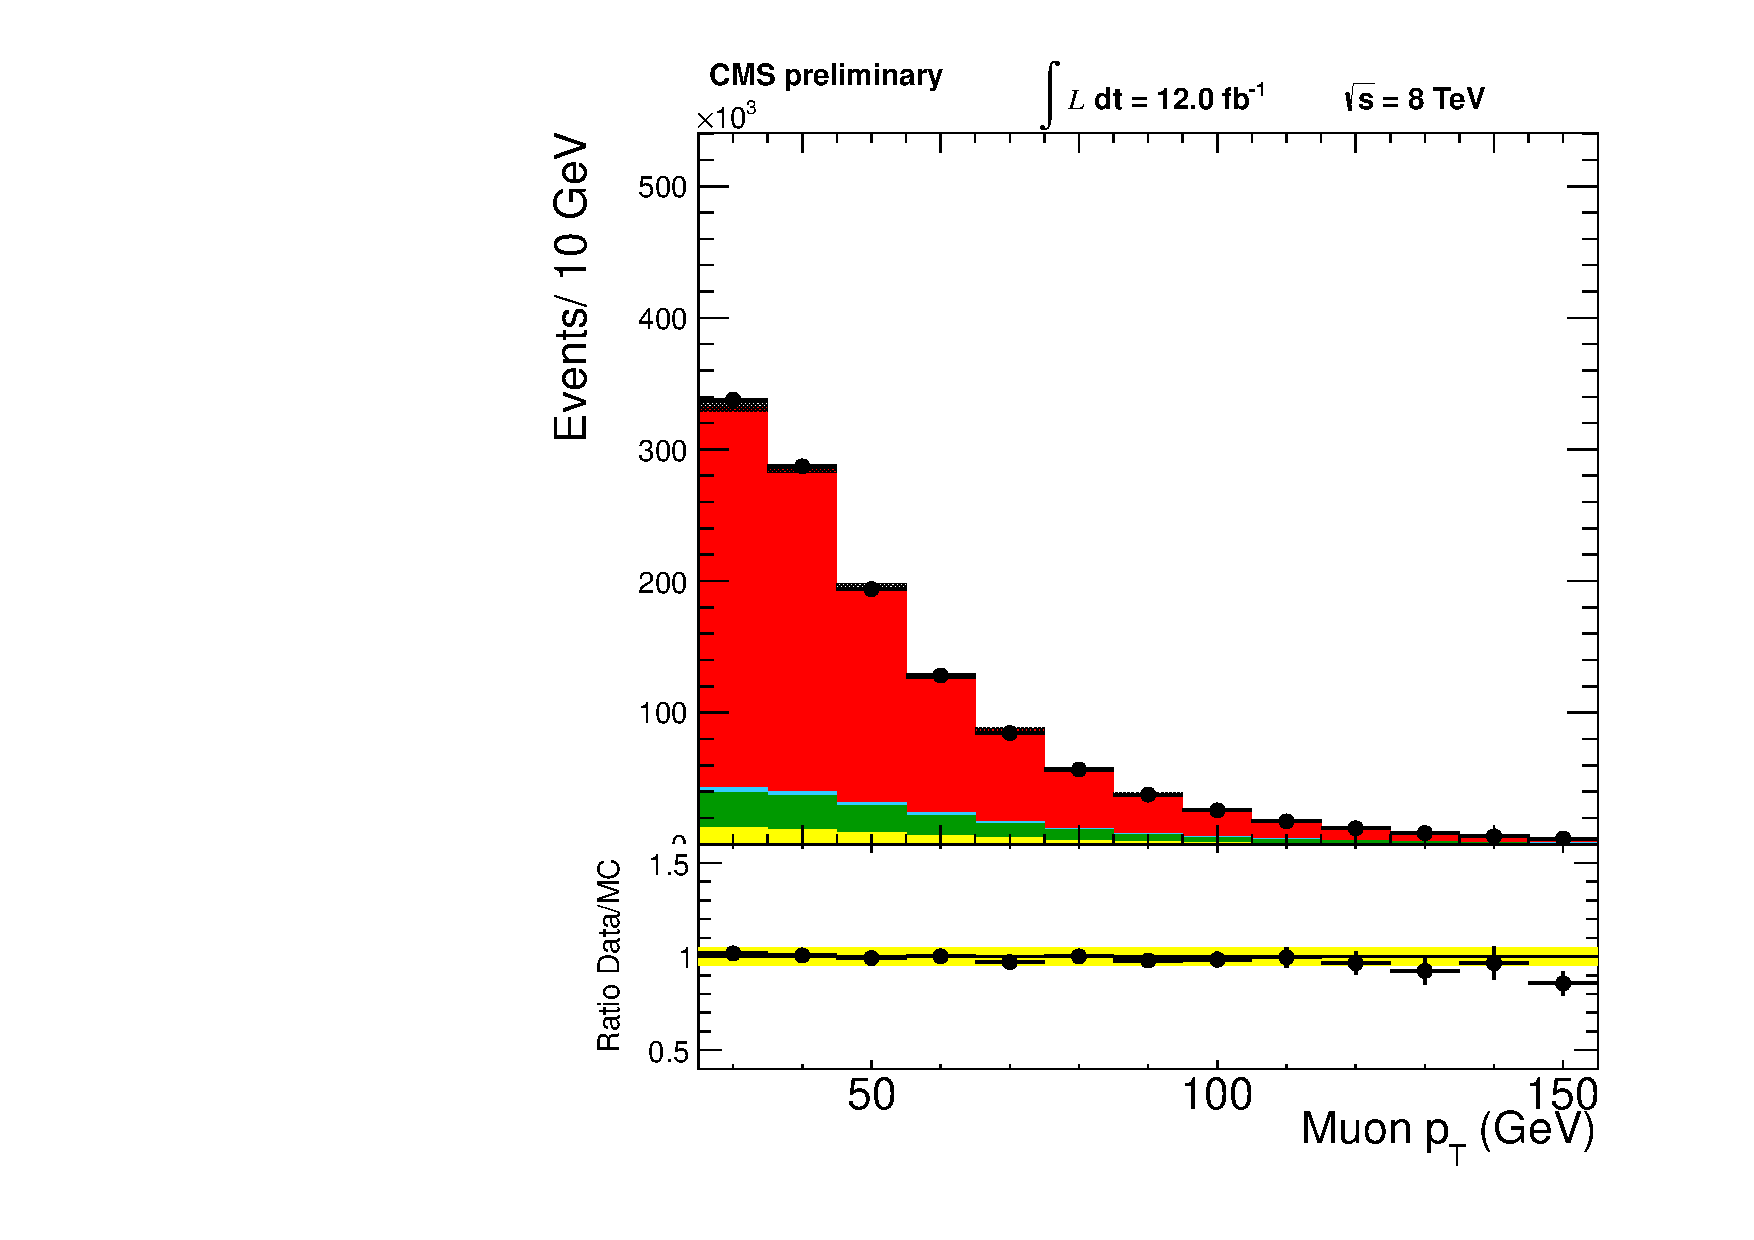
\includegraphics[width=0.49\textwidth]{plots/2012_DataMC/mu_W_muon_pt.pdf}
    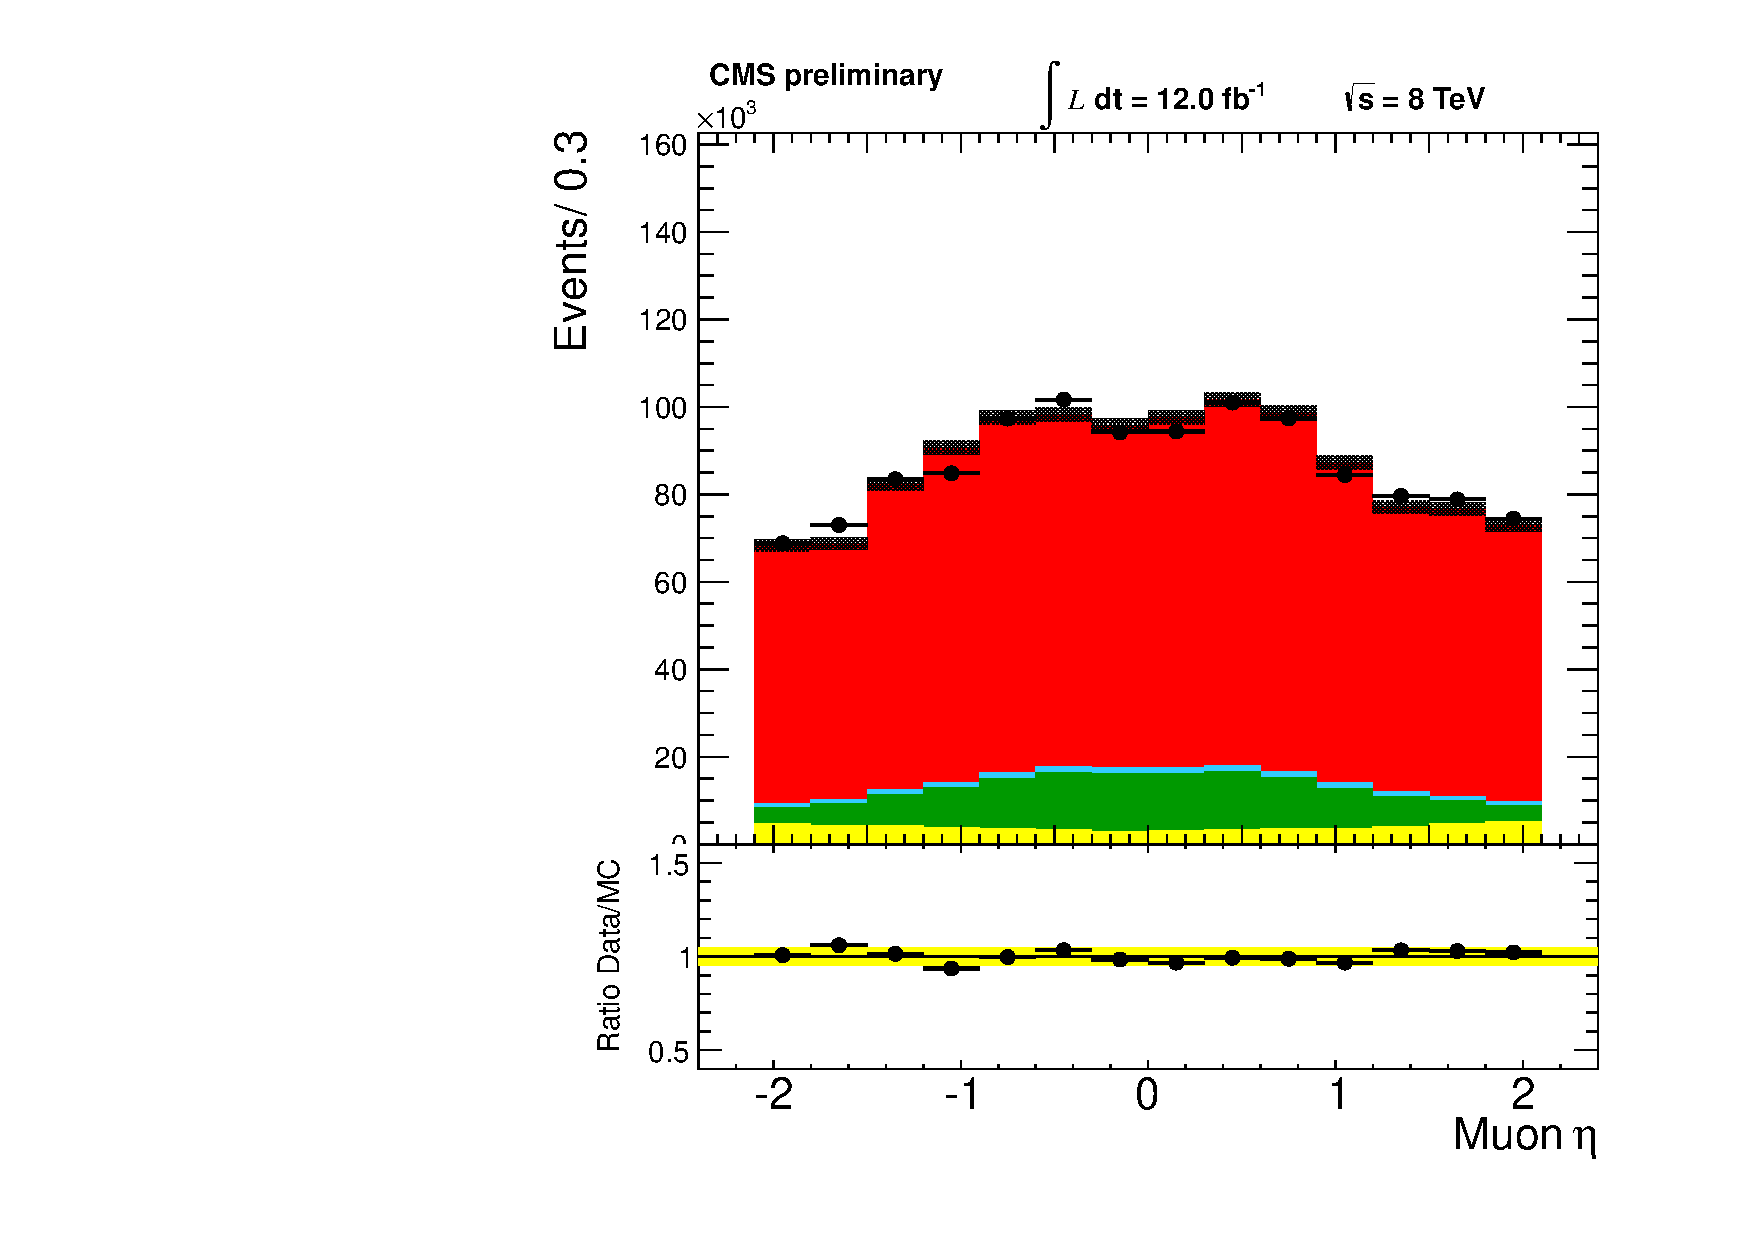
\includegraphics[width=0.49\textwidth]{plots/2012_DataMC/mu_W_muon_eta.pdf}
    \caption{Comparison of the muon $p_{T} $ (left) and the
    muon $\eta $ (right) distributions from data and MC for the
    muon+jets selection. 
    }
   \label{fig:mu_muon}}
\end{figure}

%%%%%%%%%%%%%%%%%%%%%%%%%%%%
\begin{figure}[h!t]
  {\centering
    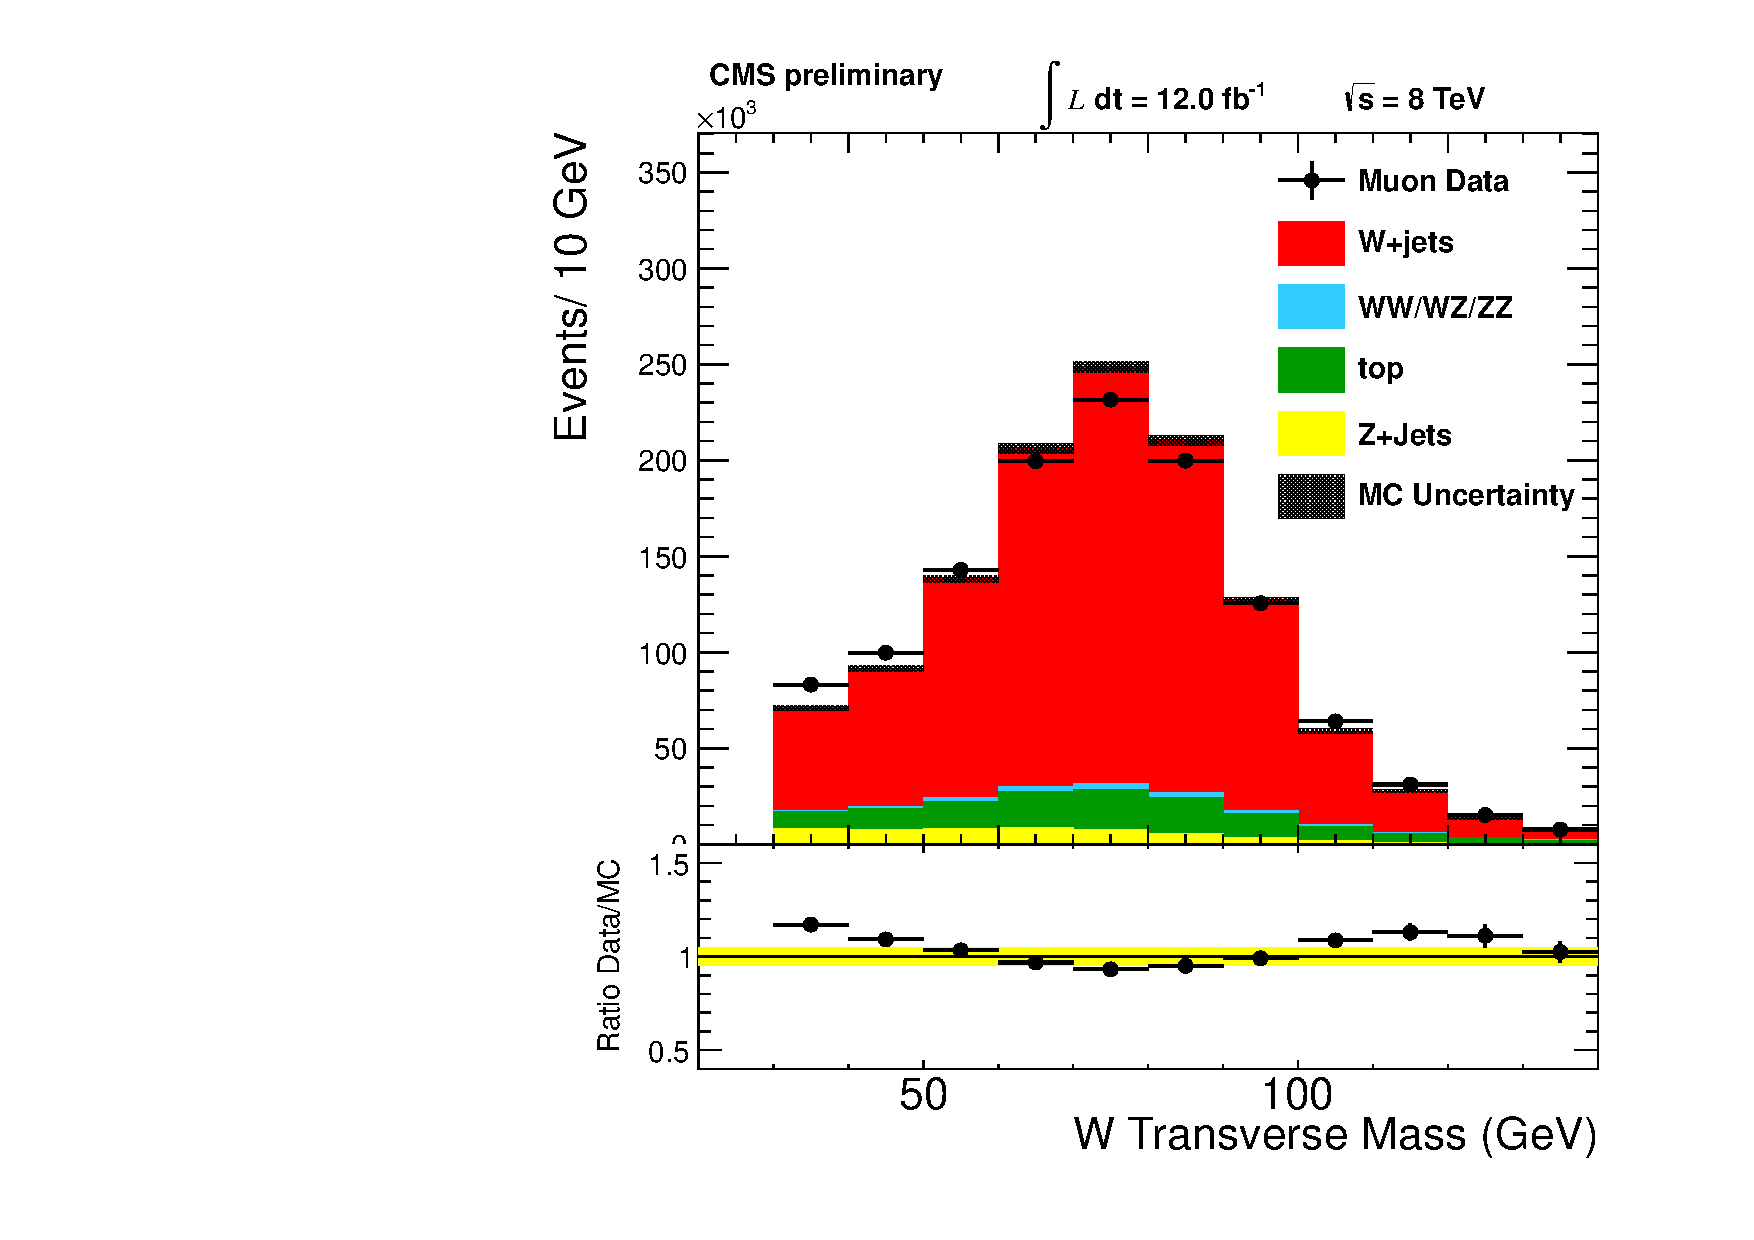
\includegraphics[width=0.49\textwidth]{plots/2012_DataMC/mu_W_mt.pdf}
    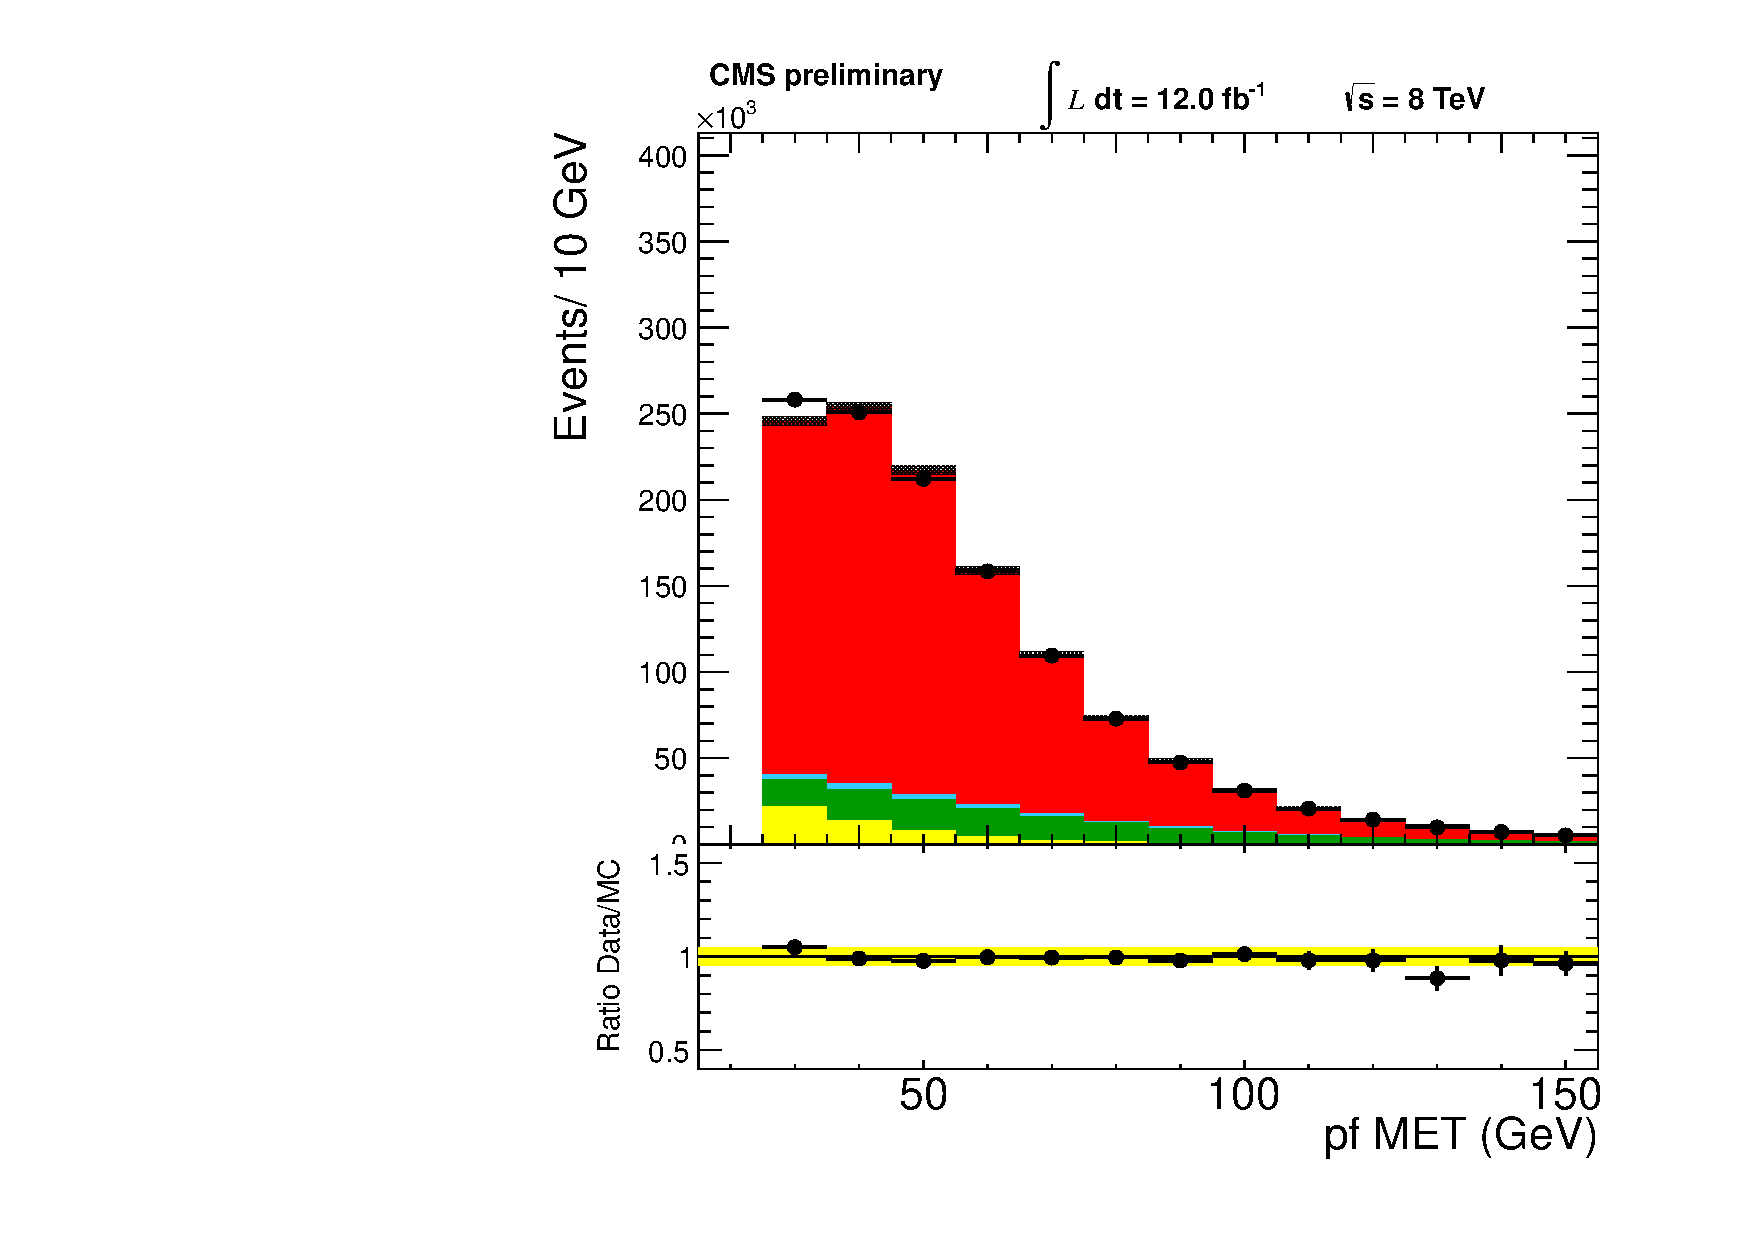
\includegraphics[width=0.49\textwidth]{plots/2012_DataMC/mu_event_met_pfmet.pdf}
    \caption{Comparison of the distributions from data and MC of the
     transverse mass of the muon / MET system (left) and the MET (right)
    for the muon+jets selection.
    }
    \label{fig:mu_W_Mt}}
\end{figure}
%%%%%%%%%%%%%%%%%%%%%%%%%%%%
\begin{figure}[h!t]
  {\centering
    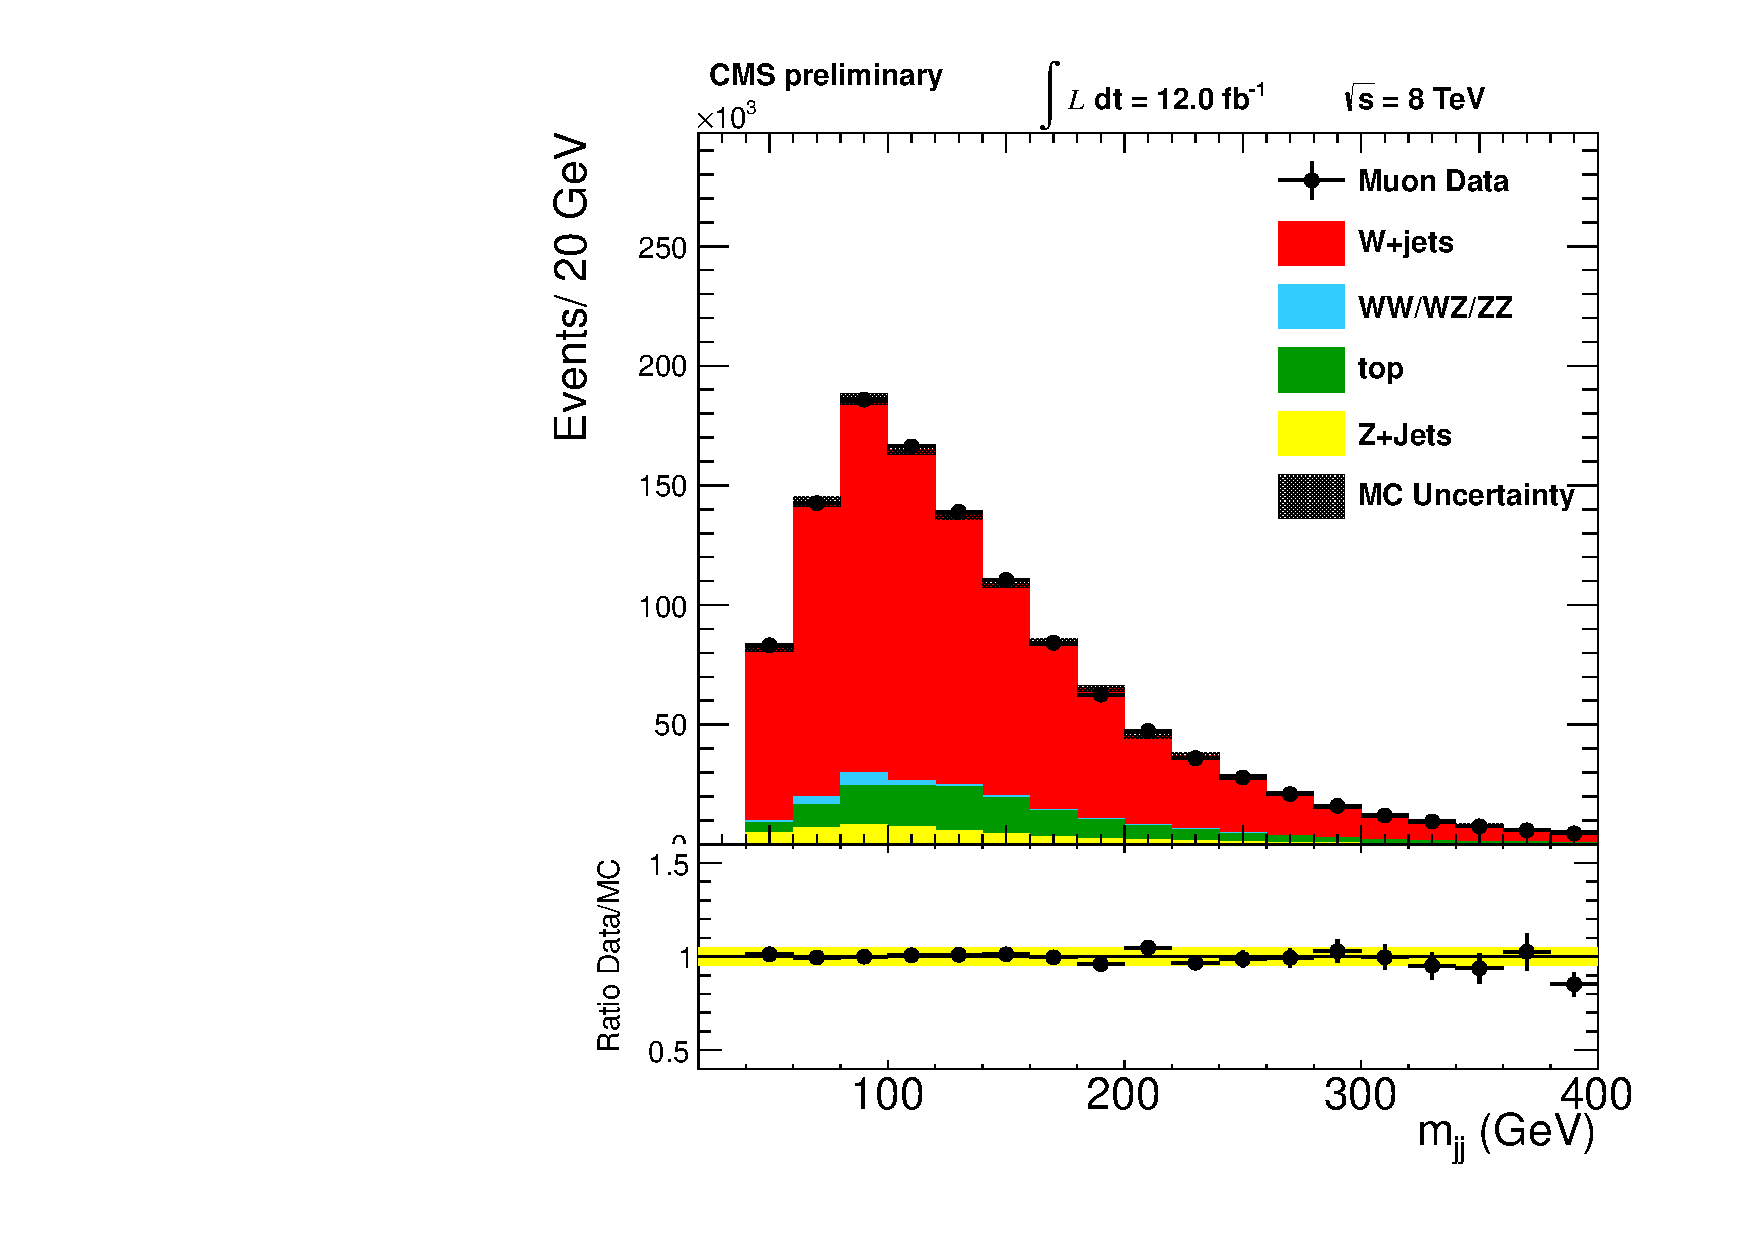
\includegraphics[width=0.49\textwidth]{plots/2012_DataMC/mu_mjj.pdf}
    \caption{Comparison of the dijet mass ($m_{JJ}$) distributions from data and MC for 
      the muon+jets selection. }
    \label{fig:mu_mjj}}
\end{figure}

%%%%%%%%%%%%%%%%%%%%%%%%%%%%
%%%%%%%%%%%%%%%%%%%%%%%%%%%%
\begin{figure}[h!t]
  {\centering
    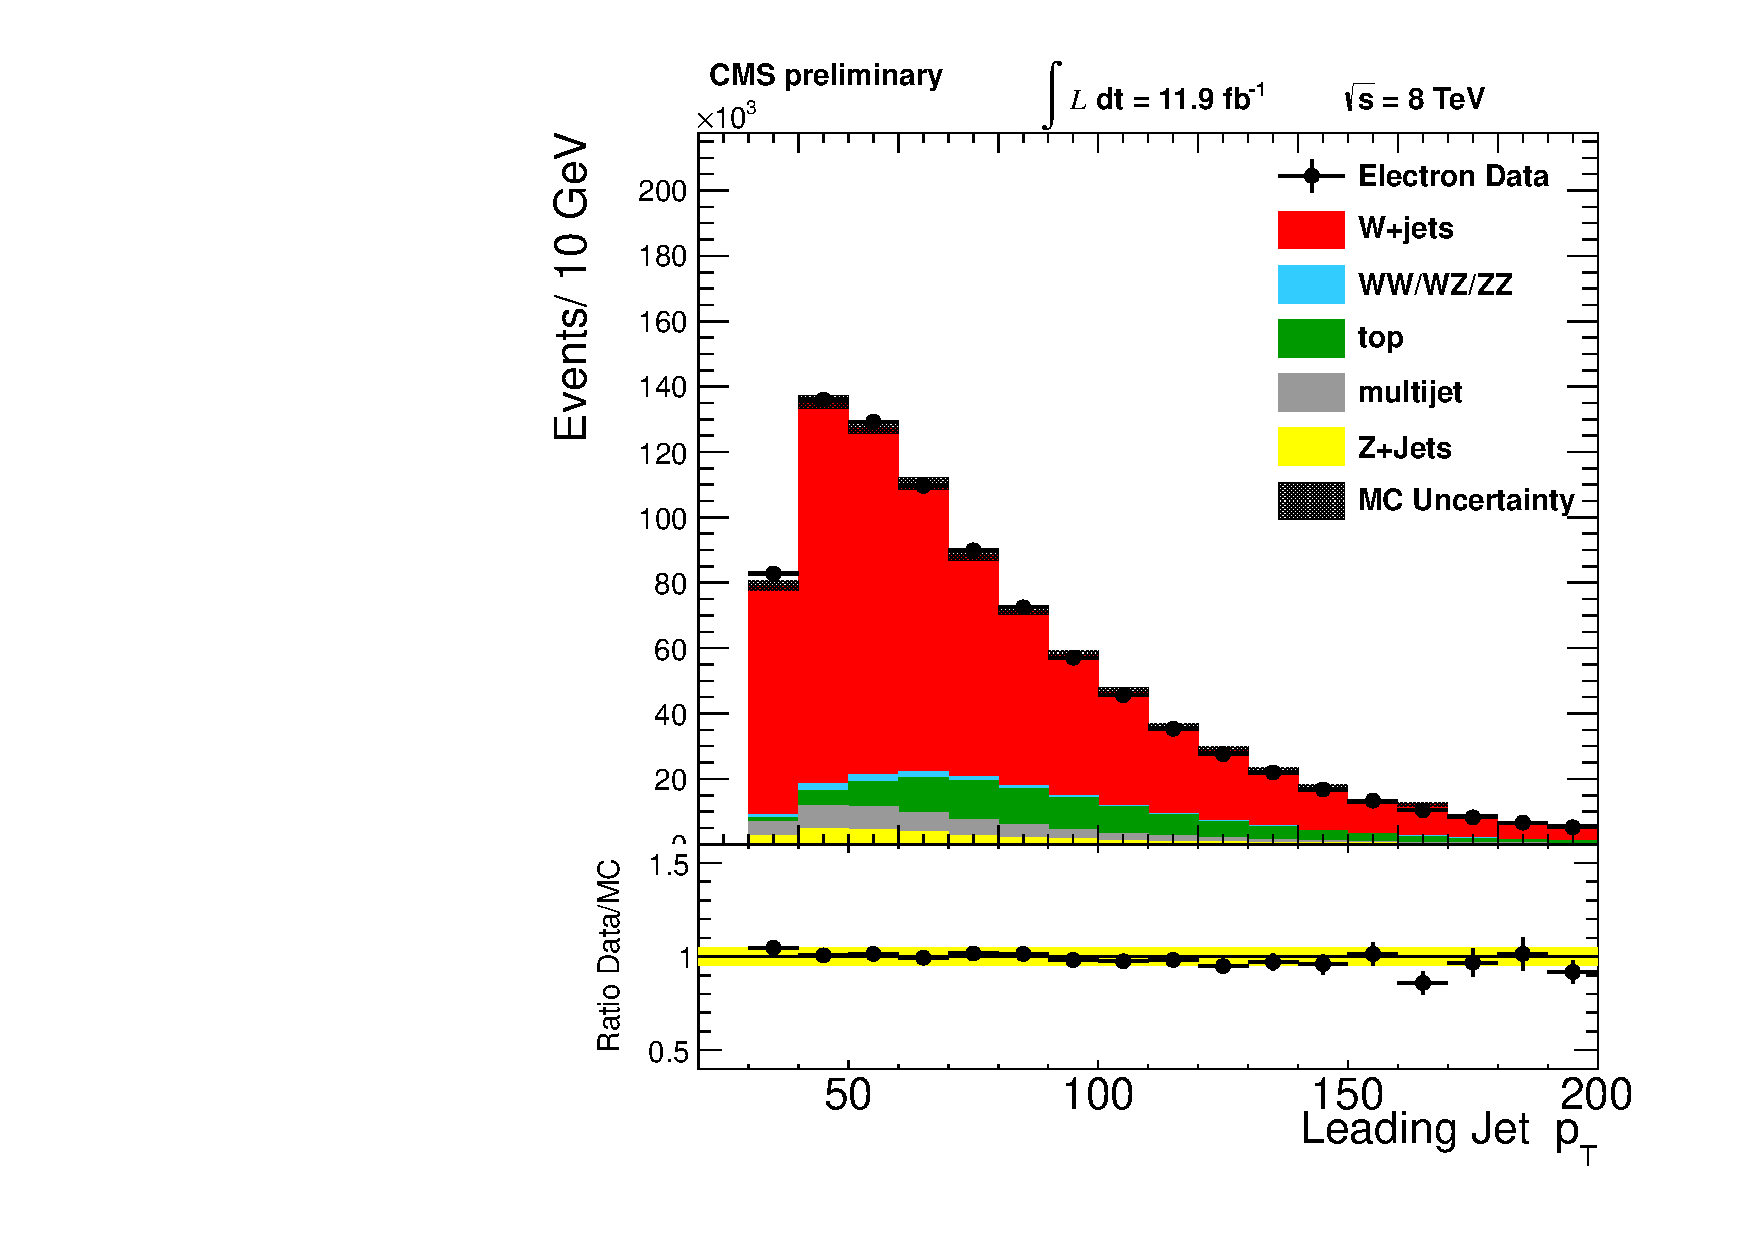
\includegraphics[width=0.49\textwidth]{plots/2012_DataMC/el_jetld_pt.pdf}
    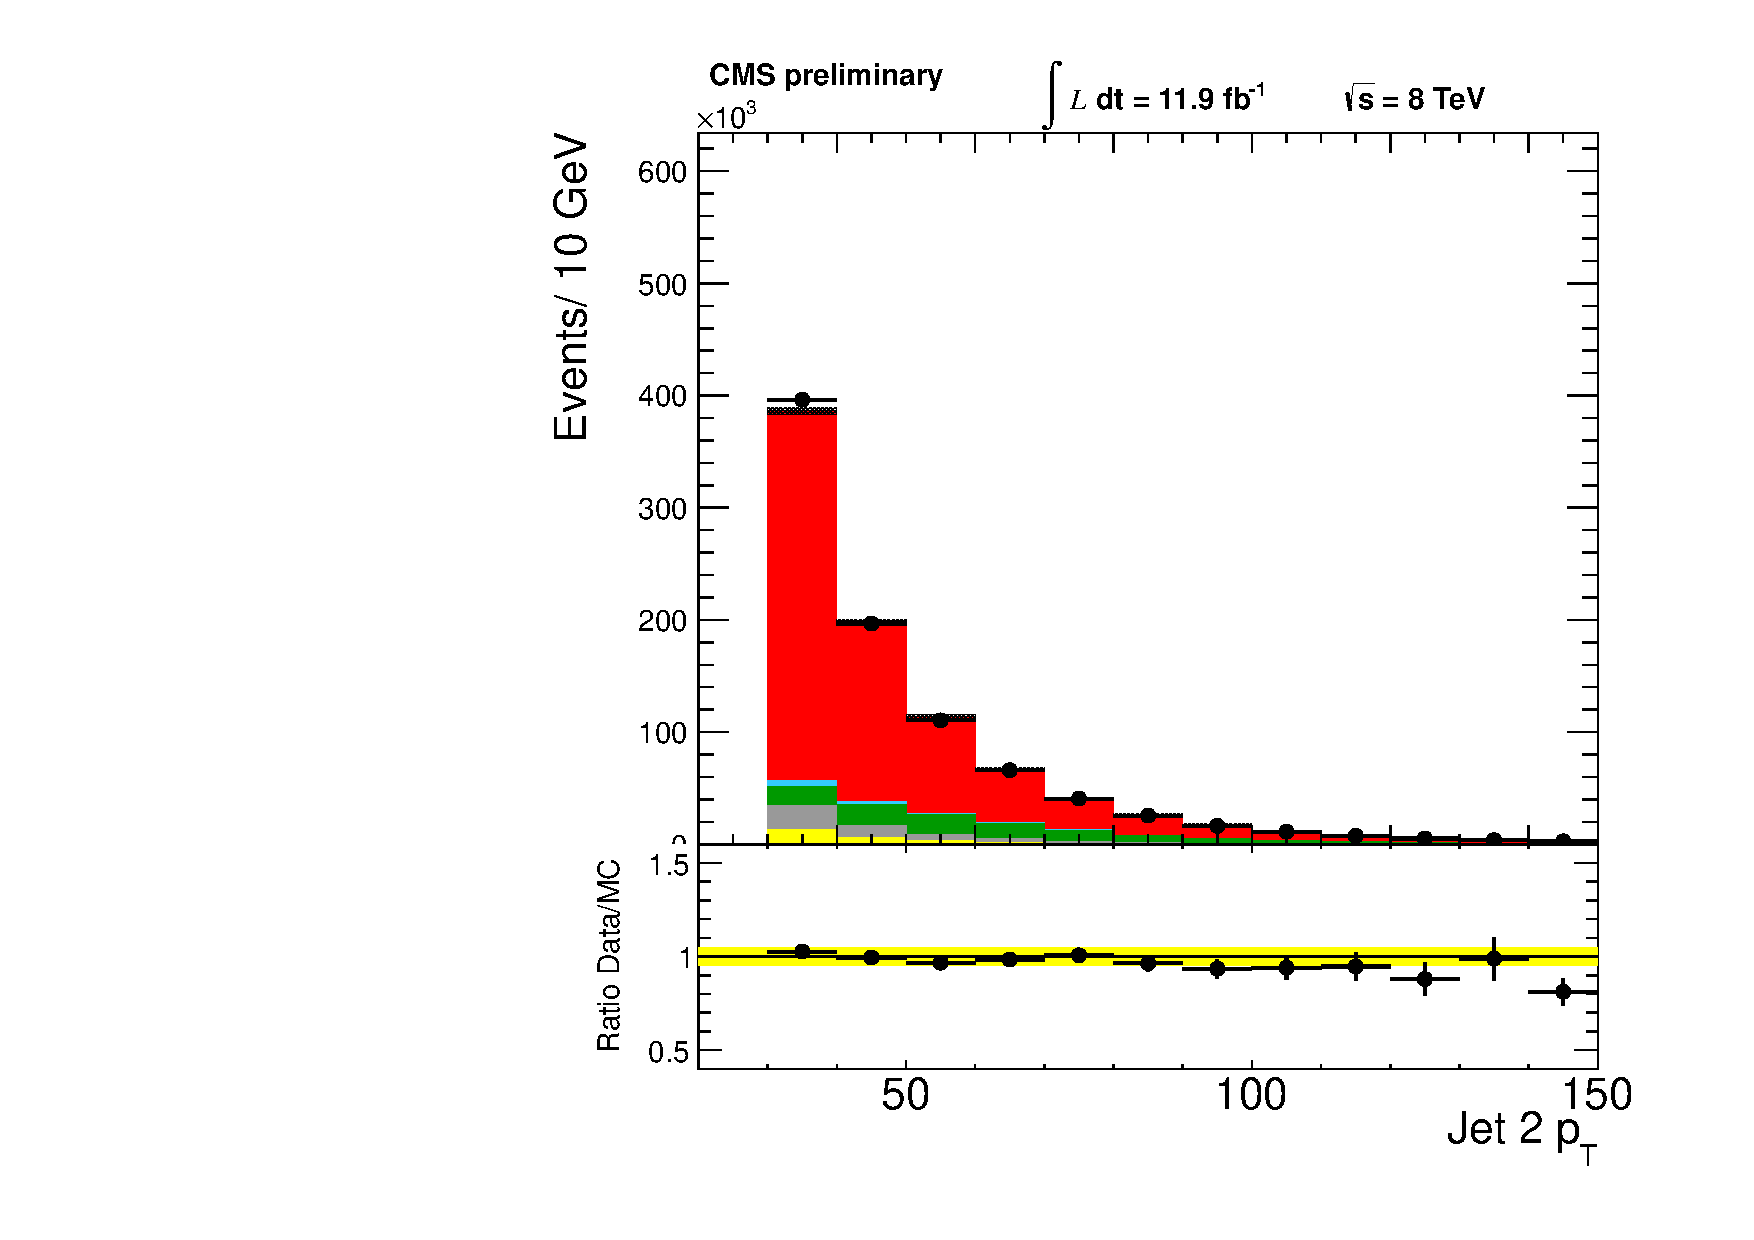
\includegraphics[width=0.49\textwidth]{plots/2012_DataMC/el_jetnt_pt.pdf}
    \caption{Comparison of the leading jet $p_{T} $ (left) and the
      second leading jet $p_{T} $ (right) distributions from data and MC
      for the electron+jets selection.}
    \label{fig:elec_jet_pt}}
\end{figure}
%%%%%%%%%%%%%%%%%%%%%%%%%%%%
\begin{figure}[h!t]
  {\centering
    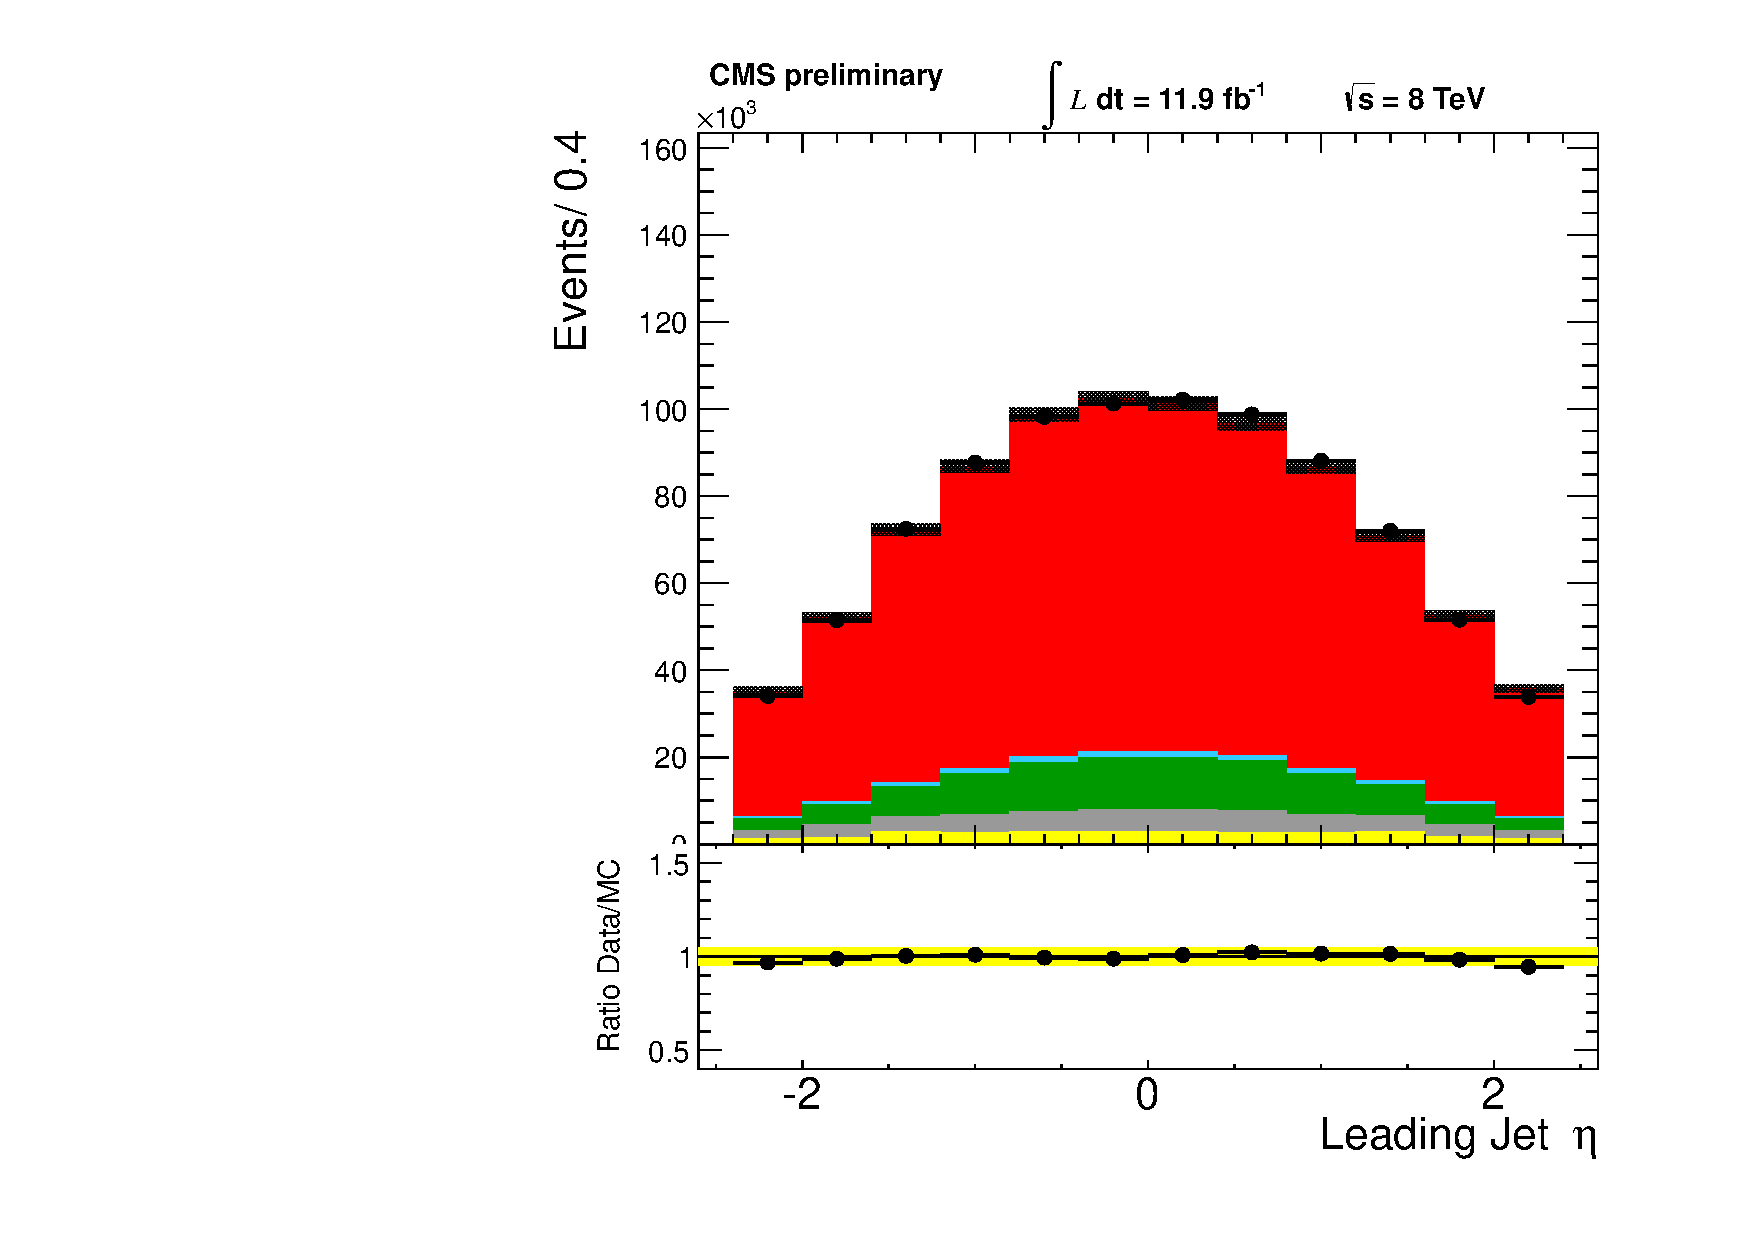
\includegraphics[width=0.49\textwidth]{plots/2012_DataMC/el_jetld_eta.pdf}
    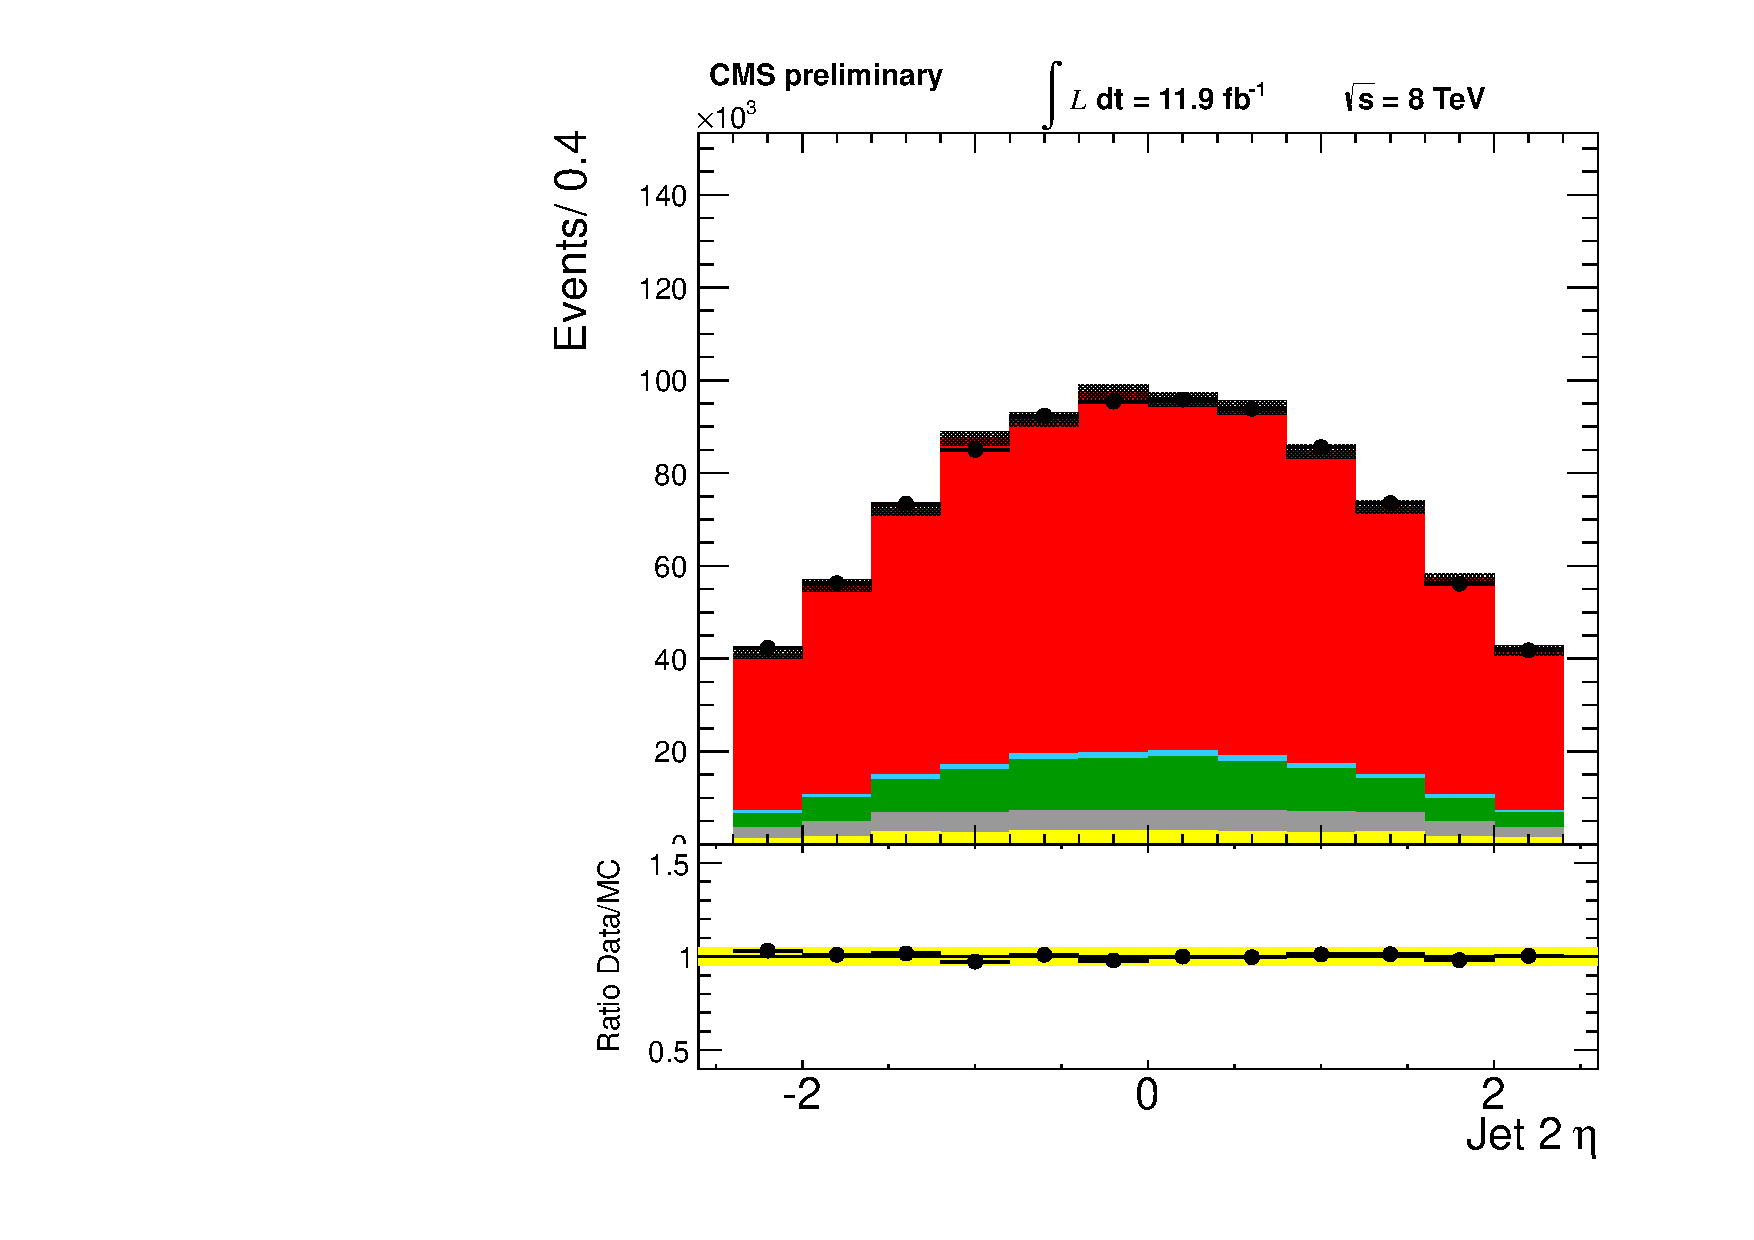
\includegraphics[width=0.49\textwidth]{plots/2012_DataMC/el_jetnt_eta.pdf}
    \caption{Comparison of the leading jet $\eta $ (left) and the
      second leading jet $\eta $ (right) distributions from data and MC for the electron+jets selection.}
    \label{fig:elec_jet_eta}}
\end{figure}
%%%%%%%%%%%%%%%%%%%%%%%%%%%%
\begin{figure}[h!t]
  {\centering
    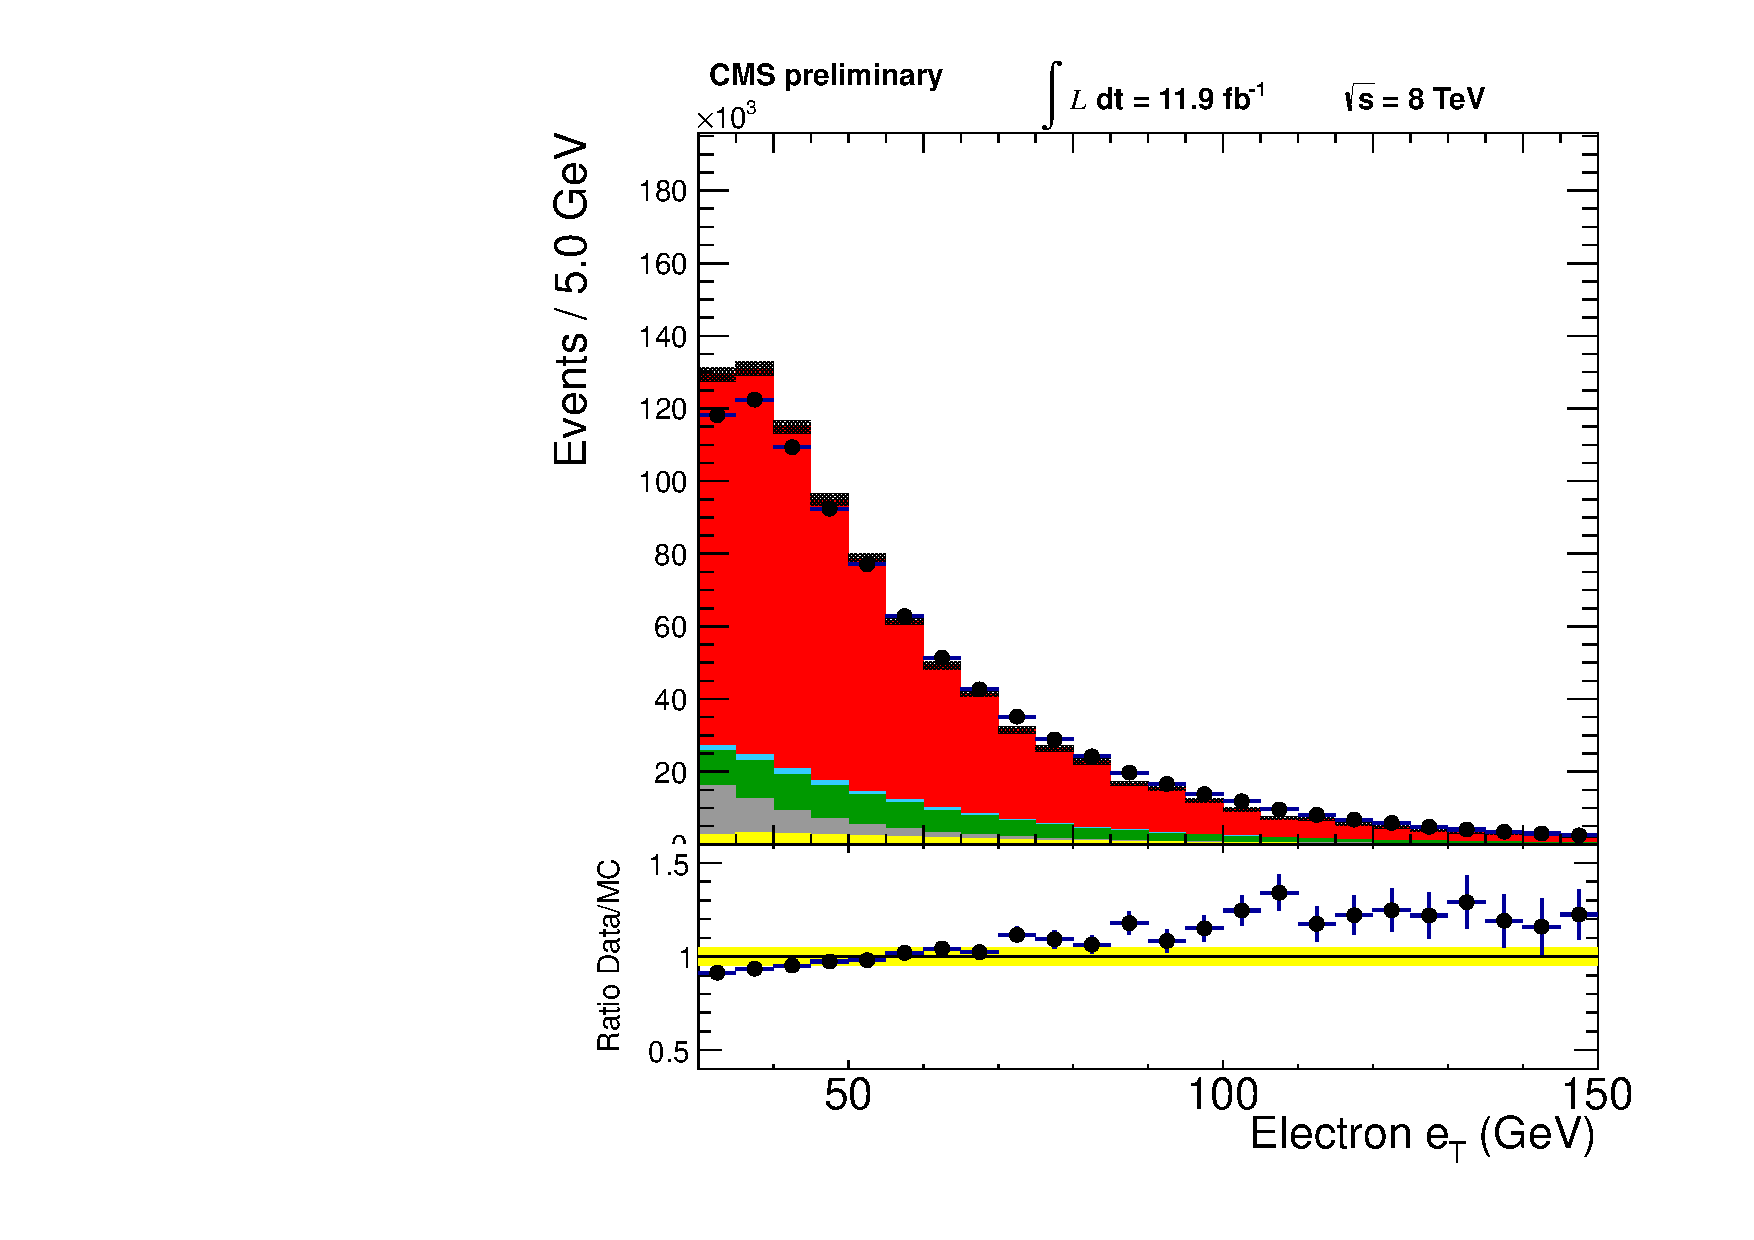
\includegraphics[width=0.49\textwidth]{plots/2012_DataMC/el_W_electron_et.pdf}
    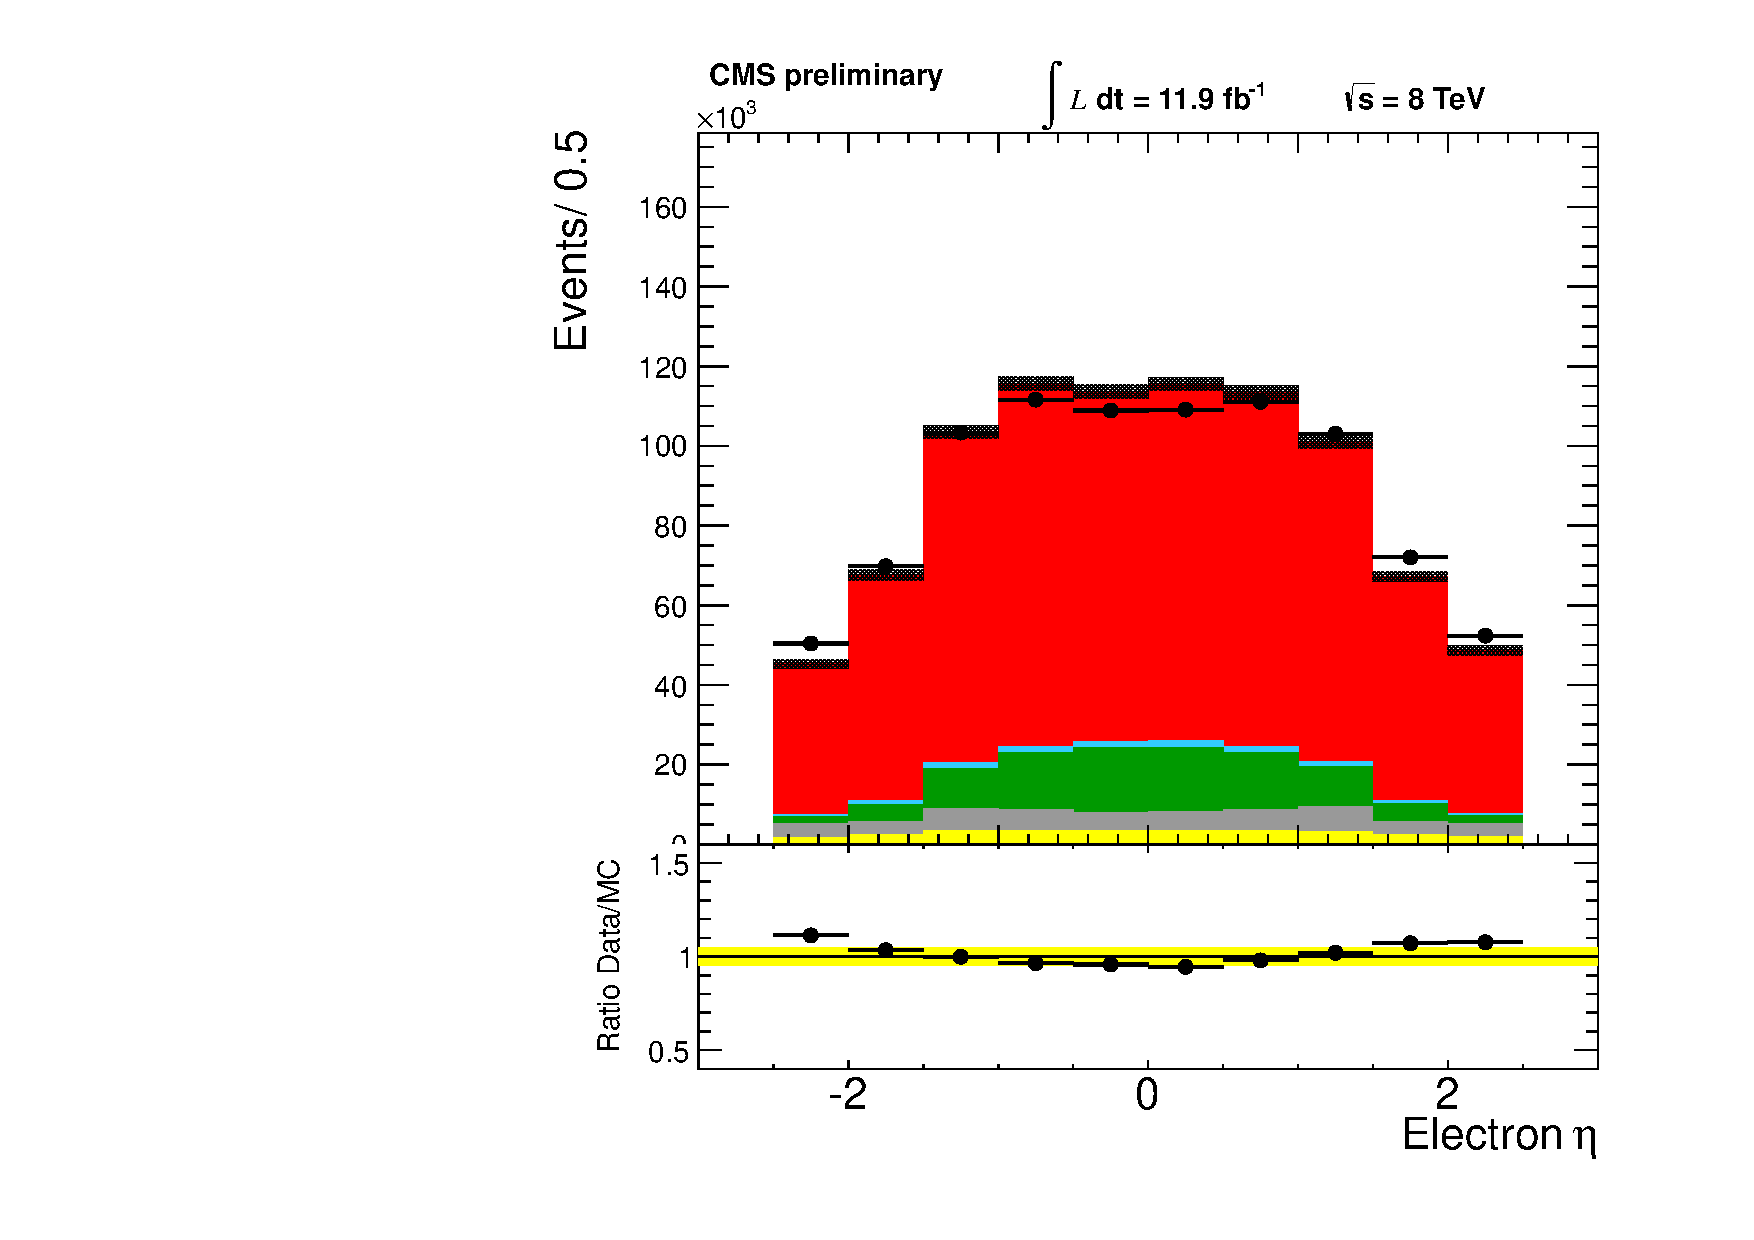
\includegraphics[width=0.49\textwidth]{plots/2012_DataMC/el_W_electron_eta.pdf}
    \caption{Comparison of the electron $E_{T} $ (left) and the
    electron $\eta $ (right) distributions from data and MC for the
    electron+jets selection. 
    }
   \label{fig:elec_electron}}
\end{figure}
%%%%%%%%%%%%%%%%%%%%%%%%%%%%
\begin{figure}[h!t]
  {\centering
    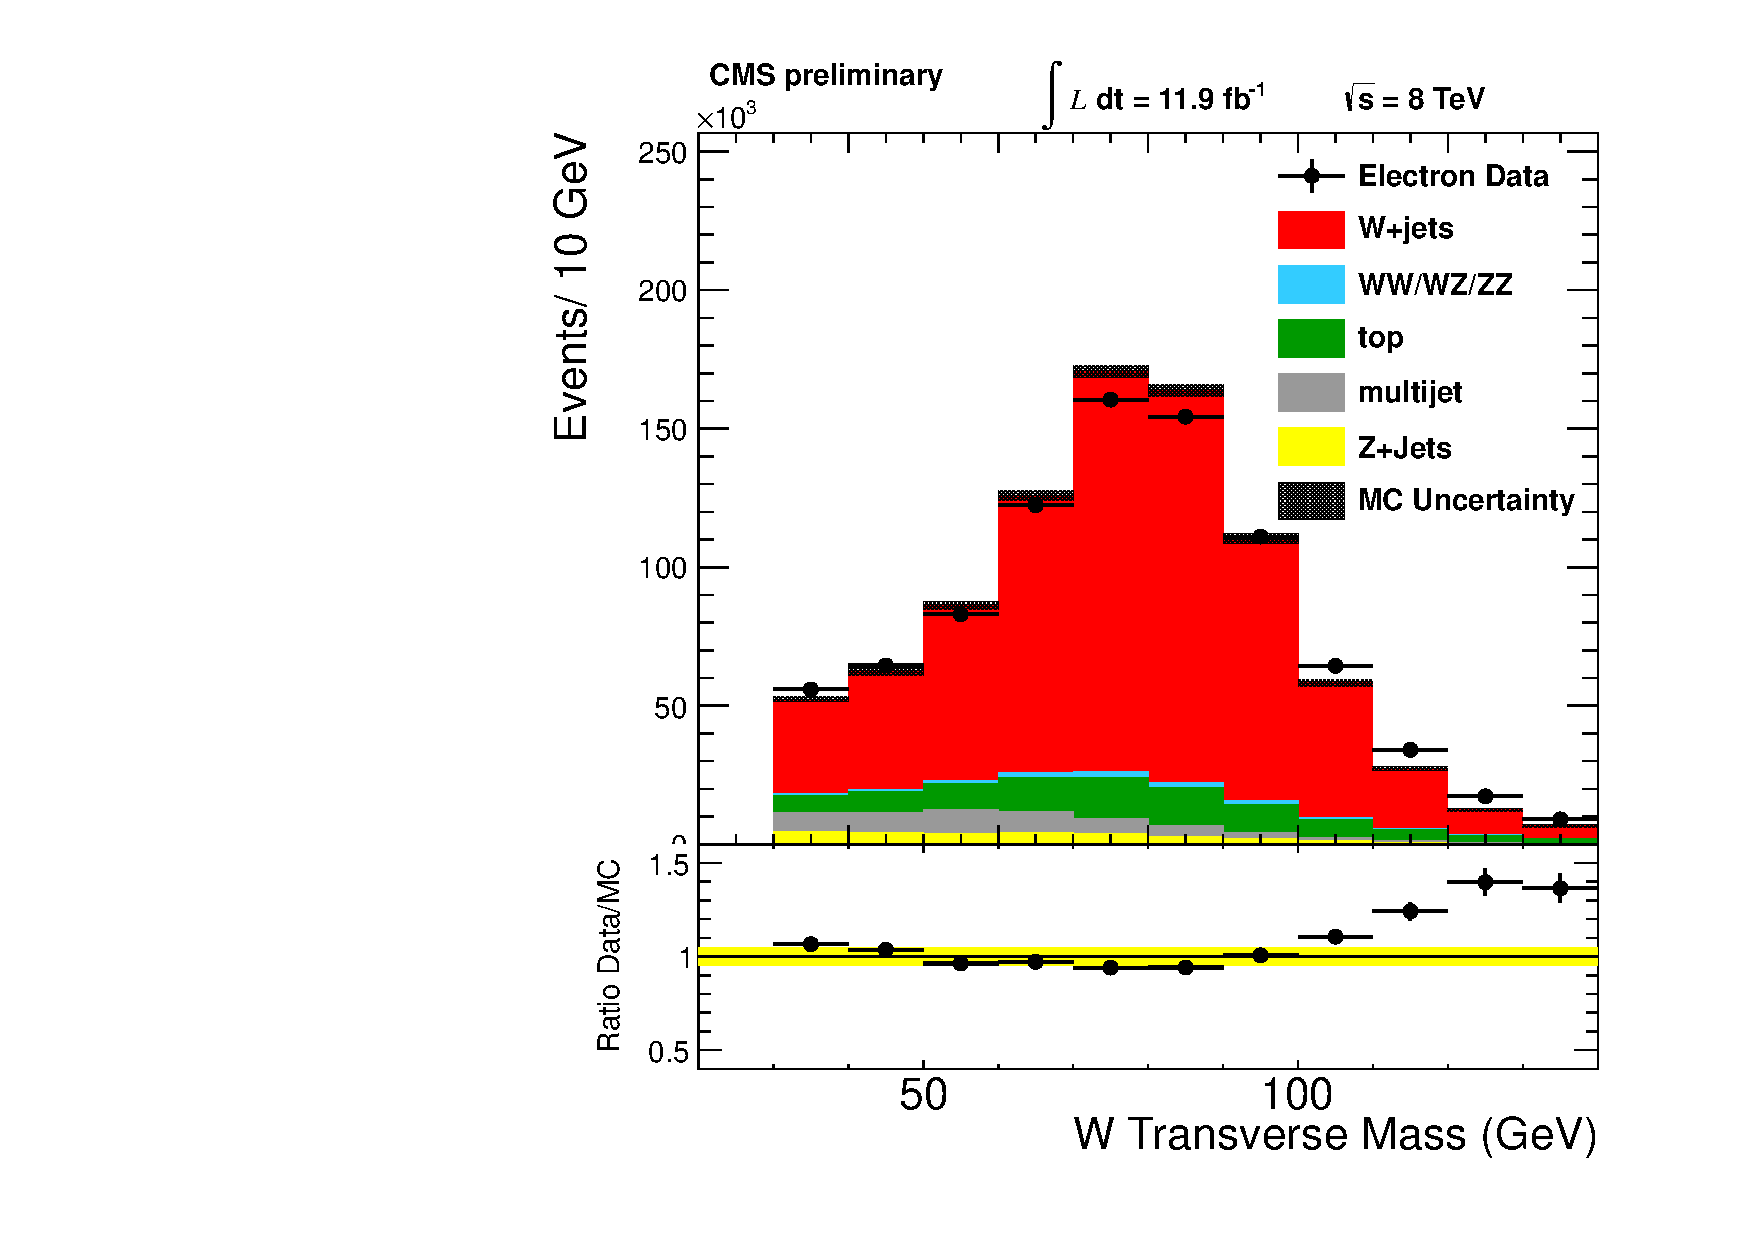
\includegraphics[width=0.49\textwidth]{plots/2012_DataMC/el_W_mt.pdf}
    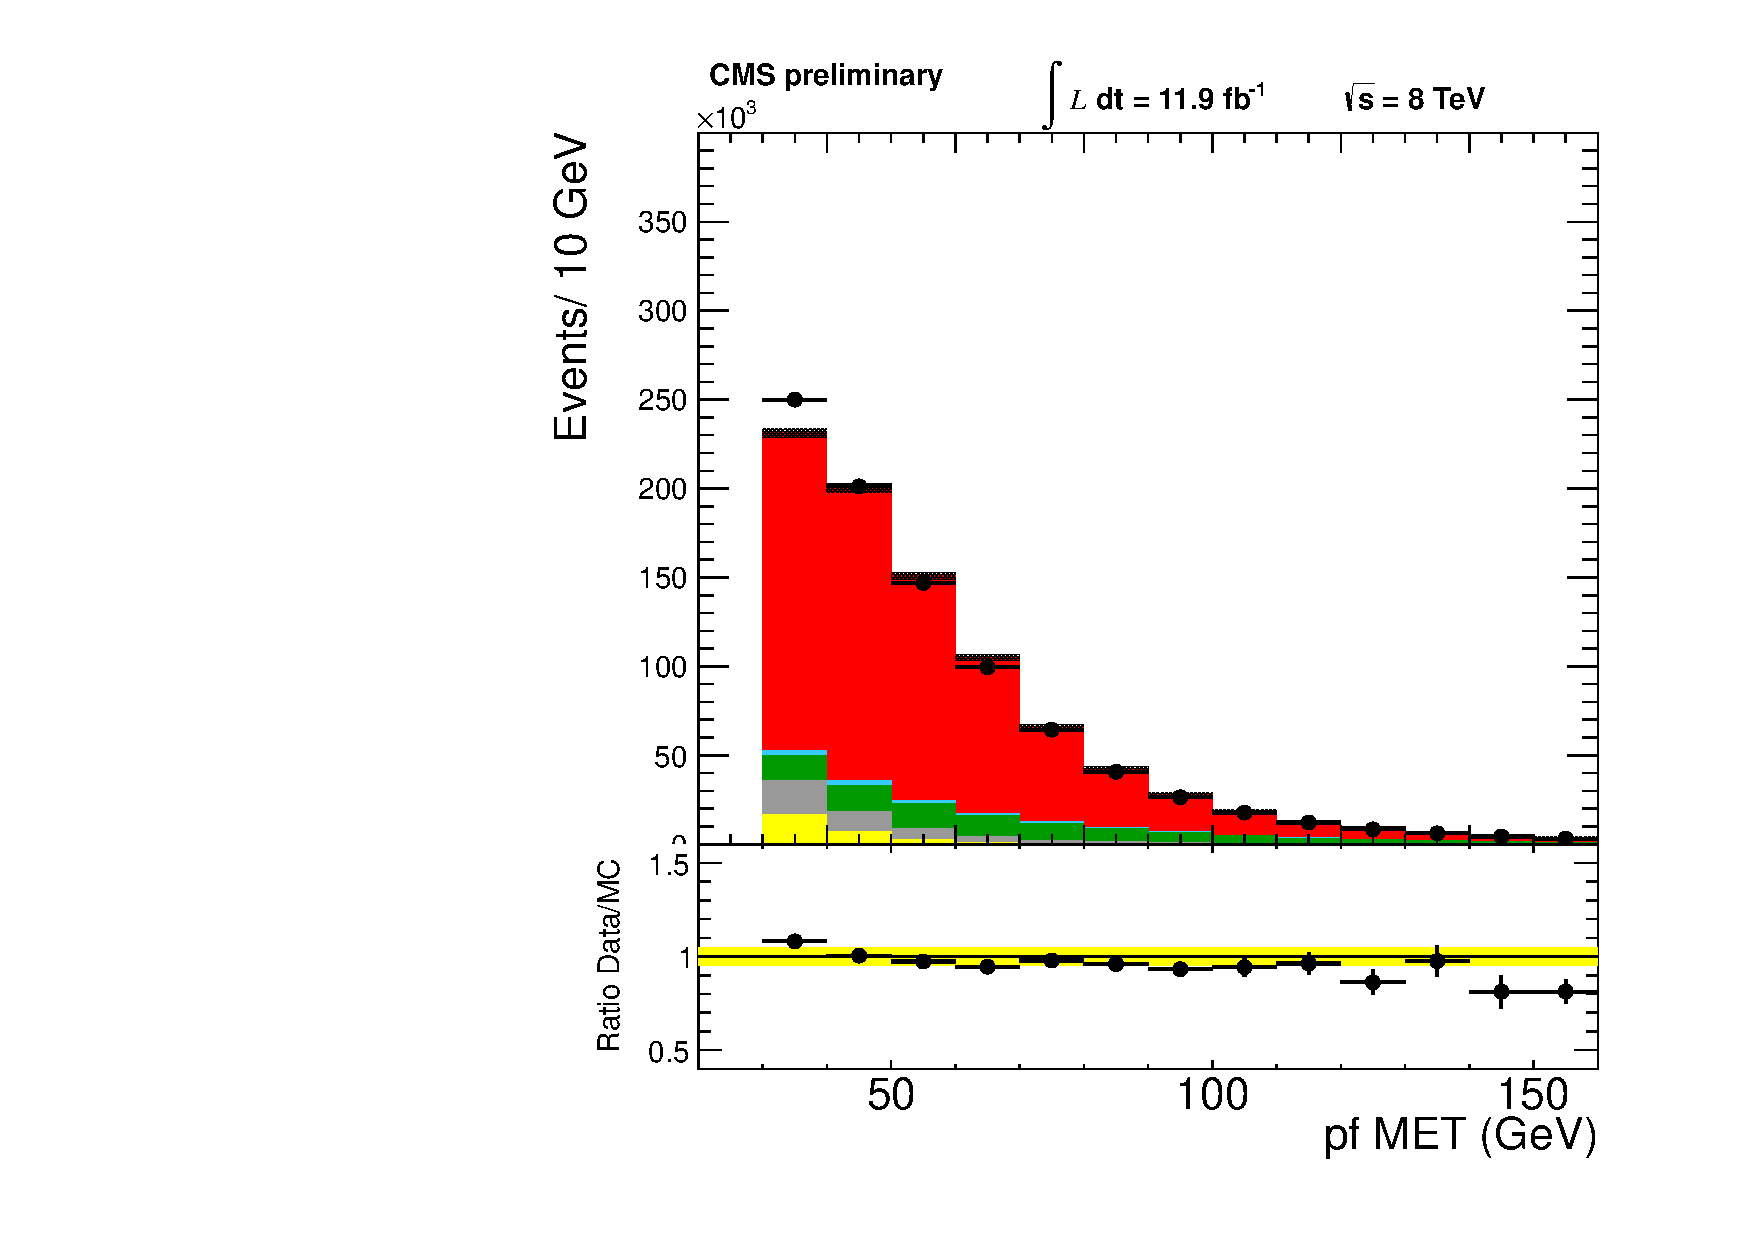
\includegraphics[width=0.49\textwidth]{plots/2012_DataMC/el_event_met_pfmet.pdf}
    \caption{Comparison of the distributions from data and MC of the transverse mass
     of electron / MET system (left) and the MET (right) for the
      electron+jets selection. 
      }
    \label{fig:elec_W_Mt}}
\end{figure}
%%%%%%%%%%%%%%%%%%%%%%%%%%%%
\begin{figure}[h!t]
  {\centering
    \includegraphics[width=0.49\textwidth]{plots/2012_DataMC/el_mjj.pdf}
    \caption{Comparison of the dijet mass ($m_{JJ}$) distributions from data and MC for 
      the electron+jets selection. }
    \label{fig:elec_mjj}}
\end{figure}
%%%%%%%%%%%%%%%%%%%%%%%%%%%%
%%%%%%%%%%%%%%%%%%%%%%%%%%%%
\clearpage
The data MC comparison for the various inputs to the MVA are shown in  
Figures ~\ref{fig:mu_theta}-\ref{fig:mu_ww}
for the muon+jets sample and in 
Figures ~\ref{fig:elec_theta}-\ref{fig:elec_ww} for
the electron+jets sample. 

% quark-gluon discriminants
%% %%%%%%%%%%%%%%%%%%%%%%%%%%%%
%% \begin{figure}[h!t]
%%   {\centering
%%     \includegraphics[width=0.49\textwidth]{plots/2012_DataMC/mu_jetld_qgl.pdf}
%%     \includegraphics[width=0.49\textwidth]{plots/2012_DataMC/mu_jetnt_qgl.pdf}
%%     \caption{Comparison of the Quark-gluon likelihood distributions for leading jet (left)
%%     second leading (right) from data and MC for the muon+jets selection.}
%% \label{fig:mu_jet_qgl}}
%% \end{figure}
% angular variables
%%%%%%%%%%%%%%%%%%%%%%%%%%%%
\begin{figure}[h!t]
  {\centering
    \includegraphics[width=0.49\textwidth]{plots/2012_DataMC/mu_ha.pdf}
    \includegraphics[width=0.49\textwidth]{plots/2012_DataMC/mu_hb.pdf}
    \caption{Comparison of the angular distributions for $\cos\theta_{1}$ (left) and
   $\cos\theta_{2}$ (right) from data and MC for the muon+jets selection.}
\label{fig:mu_theta}}
\end{figure}
%%%%%%%%%%%%%%%%%%%%%%%%%%%%
\begin{figure}[h!t]
  {\centering
     \includegraphics[width=0.49\textwidth]{plots/2012_DataMC/mu_hs.pdf}
    \caption{Comparison of the angular distributions for $\cos\theta^{\ast}$ from data and MC 
   for the muon+jets selection.}
\label{fig:mu_thetas}}
\end{figure}
%%%%%%%%%%%%%%%%%%%%%%%%%%%%
\begin{figure}[h!t]
  {\centering
    \includegraphics[width=0.49\textwidth]{plots/2012_DataMC/mu_phi.pdf}
    \includegraphics[width=0.49\textwidth]{plots/2012_DataMC/mu_phib.pdf}
    \caption{Comparison of the angular distributions for $\Phi$ (left) and $\Phi_{1}$ (right) from data and 
      MC for the muon+jets selection.}
\label{fig:mu_phi}}
\end{figure}

%%%%%%%%%%%%%%%%%%%%%%%%%%%%
\begin{figure}[h!t]
  {\centering
    \includegraphics[width=0.49\textwidth]{plots/2012_DataMC/mu_charge.pdf}
    \caption{Comparison of the charge of the muon from data and MC for the muon+jets selection.}
\label{fig:mu_chg}}
\end{figure}

% rapidity and pt of the WW system

%%%%%%%%%%%%%%%%%%%%%%%%%%%%
\begin{figure}[h!t]
  {\centering
    \includegraphics[width=0.49\textwidth]{plots/2012_DataMC/mu_ptlvjj.pdf}
    \includegraphics[width=0.49\textwidth]{plots/2012_DataMC/mu_etalvjj.pdf}
    \caption{Comparison of the $p_{T}$ (left) and $\eta$ (right) of the WW system
      from data and MC for the muon+jets selection.}
\label{fig:mu_ww}}
\end{figure}

%%%%%%%%%%%%%%%%%%%%%%%%%%%%%%%%%
%%%%%%%%%%%%%%%%%%%%%%%

% quark-gluon discriminants
%%%%%%%%%%%%%%%%%%%%%%%%%%%%
%% \begin{figure}[h!t]
%%   {\centering
%%     \includegraphics[width=0.49\textwidth]{plots/2012_DataMC/el_jetld_qgl.pdf}
%%     \includegraphics[width=0.49\textwidth]{plots/2012_DataMC/el_jetnt_qgl.pdf}
%%     \caption{Comparison of the Quark-gluon likelihood distributions for leading jet (left)
%%     second leading (right) from data and MC for the electron+jets selection.}
%% \label{fig:elec_jet_qgl}}
%% \end{figure}
% angular variables
%%%%%%%%%%%%%%%%%%%%%%%%%%%%
%%%%%%%%%%%%%%%%%%%%%%%%%%%%
\begin{figure}[h!t]
  {\centering
    \includegraphics[width=0.49\textwidth]{plots/2012_DataMC/el_ha.pdf}
    \includegraphics[width=0.49\textwidth]{plots/2012_DataMC/el_hb.pdf}
    \caption{Comparison of the angular distributions for $\cos\theta_{1}$ (left) and
   $\cos\theta_{2}$ (right) from data and MC for the electron+jets selection.}
\label{fig:elec_theta}}
\end{figure}
%%%%%%%%%%%%%%%%%%%%%%%%%%%%
\begin{figure}[h!t]
  {\centering
     \includegraphics[width=0.49\textwidth]{plots/2012_DataMC/el_hs.pdf}
    \caption{Comparison of the angular distributions for $\cos\theta^{\ast}$ from data and MC 
   for the electron+jets selection.}
\label{fig:elec_thetas}}
\end{figure}
%%%%%%%%%%%%%%%%%%%%%%%%%%%%
\begin{figure}[h!t]
  {\centering
    \includegraphics[width=0.49\textwidth]{plots/2012_DataMC/el_phi.pdf}
    \includegraphics[width=0.49\textwidth]{plots/2012_DataMC/el_phib.pdf}
    \caption{Comparison of the angular distributions for $\Phi$ (left) and
    $\Phi_{1}$ (right) from data and MC for the 
    electron+jets selection.}
\label{fig:elec_phi}}
\end{figure}

%%%%%%%%%%%%%%%%%%%%%%%%%%%%
\begin{figure}[h!t]
  {\centering
    \includegraphics[width=0.49\textwidth]{plots/2012_DataMC/el_charge.pdf}
    \caption{Comparison of the charge of the electron from data and MC for the electron+jets selection.}
\label{fig:elec_chg}}
\end{figure}

% rapidity and pt of the WW system

%%%%%%%%%%%%%%%%%%%%%%%%%%%%
\begin{figure}[h!t]
  {\centering
    \includegraphics[width=0.49\textwidth]{plots/2012_DataMC/el_ptlvjj.pdf}
    \includegraphics[width=0.49\textwidth]{plots/2012_DataMC/el_etalvjj.pdf}
    \caption{Comparison of the $p_{T}$ (left) and $\eta$ (right) of the WW system
      from data and MC for the electron+jets selection.}
\label{fig:elec_ww}}
\end{figure}

%%%%%%%%%%%%%%%%%%%%%%%%%%%%
\begin{figure}[h!t]
  {\centering
    \includegraphics[width=0.49\textwidth]{plots/2012_DataMC/el_mlvjj.pdf}
    \includegraphics[width=0.49\textwidth]{plots/2012_DataMC/mu_mlvjj.pdf}
    \caption{Comparison of the four-body invariant mass from data and MC for the electron+jets selection (left) 
             and muon+jets selection (right). The disagreement seen here between data and MC for W+jets 
	     background is the motivation for using data-driven shape for W+jets as described in 
	     Section~\ref{sec:wjetsBackground}. }
\label{fig:lep_mlvjj}}
\end{figure}

%%%%%%%%%%%%%%%%%%%%%%%%%%%%%%%%%
%%%%%%%%%%%%%%%%%%%%%%%


\clearpage{} 
\section{Lepton reconstruction, selection and trigger efficiencies}\label{sec:Eff}

Since the lepton reconstruction, selection and trigger efficiencies can be slightly different between data and simulation events,
correction factors have to be applied to the MC to account for these differences. The efficiencies are calculated using a Tag and Probe
technique exploiting Z boson decays to a pair of electrons or muons, respectively. One of the leptons is used as tag and has to pass a
tight selection, while the second one is used as probe if the tag-probe pair combines to the Z boson mass. The total lepton efficiency
can be factorized into three components:

\begin{equation}
\epsilon_{\textnormal{total}}=\epsilon_{\textnormal{Reco}}\cdot\epsilon_{\textnormal{Id}}\cdot\epsilon_{\textnormal{HLT}}
\end{equation}

The tag and probe method is nearly the same compared to the one already used in the 2011 data analysis for this Higgs search
(\cite{CMS-AN-12-029},\cite{CMS-AN-2012-021}). Therefore, only the most important information will be discussed.

\subsection{Electron efficiencies}\label{subsec:EffEle}
In the electron case, the reconstruction efficiency $\epsilon_{\textnormal{Reco}}$ characterizes the transition from a supercluster in the
electromagnetic calorimeter to a reconstructed Particle Flow electron. The ability of a reconstructed electron to pass the offline
selection consisting of several isolation and identification criteria is given by the identification efficiency $\epsilon_{\textnormal{Id}}$.
Finally, the selected electron has to fire the high level trigger. The efficiency to fulfill the HLT requirements is parametrized as
$\epsilon_{\textnormal{HLT}}$. Both in data and MC, a single electron trigger is used at HLT level. Since the efficiency depends both on $\pt$
and $\eta$ of the electron, the measurement is binned in $\pt$ as (30, 35, 40, 45, 50, 200)\GeVc and in $\eta$ as (-2.5, -1.5, 0.0, 1.5, 2.5) of
the probe electron. All three efficiency components can be calculated both for data and MC, so that a data/MC scale factor is computed
in all cases. The resulting efficiencies and scale factors are summarized in table~\ref{tab:eleEff1} and \ref{tab:eleEff2}. Figure~\ref{fig:eleEff}
shows the data/MC scale factors for the electron reconstruction (a), identification (b) and trigger (c).

\begin{table}[htb]
\centering 
\scalebox{0.70}{
  \begin{tabular}{|c|c|c|c|c|c|c|c|c|c|}
  \hline
  $p_{\textnormal{T,min}}$ & $p_{\textnormal{T,max}}$ & $\eta_{\textnormal{min}}$ & $\eta_{\textnormal{max}}$ & $\epsilon_{\textnormal{Reco,data}}$ & $\epsilon_{\textnormal{Reco,mc}}$ & $\textnormal{SF}_{\textnormal{Reco}}$ & $\epsilon_{\textnormal{ID,data}}$ & $\epsilon_{\textnormal{ID,mc}}$ & $\textnormal{SF}_{\textnormal{ID}}$ \\
  $[\GeVc]$         & $[\GeVc]$         &                     &                     &                              &                           &                                 &                            &                          &                                \\
  \hline
  \hline
  30	& 35	& -2.5	& -1.5	& 0.983$\pm$0.005 & 0.946$\pm$0.007 & 1.039$\pm$0.010 & 0.582$\pm$0.004 & 0.576$\pm$0.013 & 1.010$\pm$0.023 \\
  30	& 35	& -1.5	& 0	& 0.990$\pm$0.003 & 0.989$\pm$0.002 & 1.001$\pm$0.003 & 0.804$\pm$0.004 & 0.809$\pm$0.006 & 0.994$\pm$0.009 \\
  30	& 35	& 0	& 1.5	& 0.991$\pm$0.006 & 0.987$\pm$0.002 & 1.004$\pm$0.006 & 0.812$\pm$0.004 & 0.813$\pm$0.006 & 0.998$\pm$0.009 \\
  30	& 35	& 1.5	& 2.5	& 0.984$\pm$0.005 & 0.953$\pm$0.007 & 1.032$\pm$0.009 & 0.582$\pm$0.066 & 0.590$\pm$0.013 & 0.987$\pm$0.113 \\
  35	& 40	& -2.5	& -1.5	& 0.984$\pm$0.003 & 0.955$\pm$0.004 & 1.030$\pm$0.006 & 0.684$\pm$0.006 & 0.690$\pm$0.005 & 0.990$\pm$0.011 \\
  35	& 40	& -1.5	& 0	& 0.998$\pm$0.001 & 0.994$\pm$0.001 & 1.003$\pm$0.001 & 0.877$\pm$0.003 & 0.881$\pm$0.004 & 0.996$\pm$0.005 \\
  35	& 40	& 0	& 1.5	& 0.997$\pm$0.001 & 0.995$\pm$0.001 & 1.002$\pm$0.001 & 0.874$\pm$0.003 & 0.883$\pm$0.004 & 0.991$\pm$0.005 \\
  35	& 40	& 1.5	& 2.5	& 0.986$\pm$0.003 & 0.969$\pm$0.004 & 1.018$\pm$0.006 & 0.700$\pm$0.007 & 0.688$\pm$0.009 & 1.018$\pm$0.017 \\
  40	& 45	& -2.5	& -1.5	& 0.991$\pm$0.002 & 0.969$\pm$0.004 & 1.023$\pm$0.004 & 0.752$\pm$0.005 & 0.735$\pm$0.008 & 1.023$\pm$0.013 \\
  40	& 45	& -1.5	& 0	& 0.999$\pm$0.001 & 0.997$\pm$0.001 & 1.001$\pm$0.001 & 0.905$\pm$0.002 & 0.907$\pm$0.003 & 0.998$\pm$0.004 \\
  40	& 45	& 0	& 1.5	& 0.998$\pm$0.001 & 0.997$\pm$0.001 & 1.000$\pm$0.001 & 0.909$\pm$0.002 & 0.903$\pm$0.050 & 1.007$\pm$0.056 \\
  40	& 45	& 1.5	& 2.5	& 0.995$\pm$0.003 & 0.982$\pm$0.003 & 1.013$\pm$0.004 & 0.751$\pm$0.006 & 0.737$\pm$0.008 & 1.018$\pm$0.013 \\
  45	& 50	& -2.5	& -1.5	& 0.984$\pm$0.003 & 0.967$\pm$0.004 & 1.017$\pm$0.005 & 0.784$\pm$0.006 & 0.779$\pm$0.008 & 1.006$\pm$0.013 \\
  45	& 50	& -1.5	& 0	& 0.999$\pm$0.001 & 0.998$\pm$0.001 & 1.001$\pm$0.001 & 0.920$\pm$0.002 & 0.924$\pm$0.003 & 0.996$\pm$0.004 \\
  45	& 50	& 0	& 1.5	& 0.999$\pm$0.001 & 0.999$\pm$0.001 & 1.001$\pm$0.001 & 0.922$\pm$0.002 & 0.918$\pm$0.003 & 1.004$\pm$0.004 \\
  45	& 50	& 1.5	& 2.5	& 0.986$\pm$0.008 & 0.974$\pm$0.004 & 1.012$\pm$0.009 & 0.795$\pm$0.006 & 0.787$\pm$0.008 & 1.010$\pm$0.013 \\
  50	& 200	& -2.5	& -1.5	& 0.978$\pm$0.003 & 0.961$\pm$0.004 & 1.018$\pm$0.006 & 0.832$\pm$0.007 & 0.820$\pm$0.009 & 1.015$\pm$0.015 \\
  50	& 200	& -1.5	& 0	& 1.000$\pm$0.001 & 0.999$\pm$0.001 & 1.000$\pm$0.001 & 0.939$\pm$0.003 & 0.932$\pm$0.004 & 1.008$\pm$0.005 \\
  50	& 200	& 0	& 1.5	& 0.997$\pm$0.002 & 1.000$\pm$0.000 & 0.997$\pm$0.002 & 0.939$\pm$0.003 & 0.942$\pm$0.003 & 0.997$\pm$0.004 \\
  50	& 200	& 1.5	& 2.5	& 0.982$\pm$0.003 & 0.962$\pm$0.005 & 1.020$\pm$0.006 & 0.840$\pm$0.007 & 0.840$\pm$0.009 & 0.999$\pm$0.014 \\
  \hline
  \end{tabular}}
\caption{Electron reconstruction and selection efficiencies for data and MC and corresponding scale factors (SF). The errors are statistical only.} 
\label{tab:eleEff1} 
\end{table}

\begin{table}[htb]
\centering 
\scalebox{0.70}{
  \begin{tabular}{|c|c|c|c|c|c|c|c|c|c|}
  \hline
  $p_{\textnormal{T,min}}$ & $p_{\textnormal{T,max}}$ & $\eta_{\textnormal{min}}$ & $\eta_{\textnormal{max}}$ & $\epsilon_{\textnormal{HLT,data}}$ & $\epsilon_{\textnormal{HLT,mc}}$ & $\textnormal{SF}_{\textnormal{HLT}}$ \\
  $[\GeVc]$         & $[\GeVc]$         &                     &                     &                              &                           &                               \\
  \hline
  \hline
  30	& 35	& -2.5	& -1.5	& 0.612$\pm$0.010 & 0.659$\pm$0.015 & 0.929$\pm$0.026 \\
  30	& 35	& -1.5	& 0	& 0.866$\pm$0.003 & 0.859$\pm$0.005 & 1.007$\pm$0.007 \\
  30	& 35	& 0	& 1.5	& 0.861$\pm$0.003 & 0.870$\pm$0.005 & 0.990$\pm$0.007 \\
  30	& 35	& 1.5	& 2.5	& 0.586$\pm$0.010 & 0.637$\pm$0.015 & 0.921$\pm$0.027 \\
  35	& 40	& -2.5	& -1.5	& 0.698$\pm$0.007 & 0.681$\pm$0.011 & 1.025$\pm$0.019 \\
  35	& 40	& -1.5	& 0	& 0.891$\pm$0.002 & 0.888$\pm$0.004 & 1.004$\pm$0.005 \\
  35	& 40	& 0	& 1.5	& 0.881$\pm$0.002 & 0.887$\pm$0.004 & 0.994$\pm$0.005 \\
  35	& 40	& 1.5	& 2.5	& 0.669$\pm$0.008 & 0.693$\pm$0.011 & 0.966$\pm$0.019 \\
  40	& 45	& -2.5	& -1.5	& 0.726$\pm$0.006 & 0.718$\pm$0.009 & 1.011$\pm$0.016 \\
  40	& 45	& -1.5	& 0	& 0.900$\pm$0.002 & 0.905$\pm$0.003 & 0.994$\pm$0.004 \\
  40	& 45	& 0	& 1.5	& 0.896$\pm$0.002 & 0.902$\pm$0.003 & 0.993$\pm$0.004 \\
  40	& 45	& 1.5	& 2.5	& 0.702$\pm$0.007 & 0.739$\pm$0.009 & 0.951$\pm$0.015 \\
  45	& 50	& -2.5	& -1.5	& 0.734$\pm$0.007 & 0.768$\pm$0.009 & 0.956$\pm$0.015 \\
  45	& 50	& -1.5	& 0	& 0.910$\pm$0.002 & 0.910$\pm$0.003 & 1.001$\pm$0.005 \\
  45	& 50	& 0	& 1.5	& 0.901$\pm$0.003 & 0.909$\pm$0.003 & 0.991$\pm$0.005 \\
  45	& 50	& 1.5	& 2.5	& 0.700$\pm$0.007 & 0.755$\pm$0.010 & 0.927$\pm$0.016 \\
  50	& 200	& -2.5	& -1.5	& 0.755$\pm$0.007 & 0.765$\pm$0.010 & 0.988$\pm$0.016 \\
  50	& 200	& -1.5	& 0	& 0.918$\pm$0.003 & 0.917$\pm$0.004 & 1.000$\pm$0.005 \\
  50	& 200	& 0	& 1.5	& 0.909$\pm$0.003 & 0.922$\pm$0.003 & 0.986$\pm$0.005 \\
  50	& 200	& 1.5	& 2.5	& 0.728$\pm$0.007 & 0.767$\pm$0.010 & 0.949$\pm$0.016 \\
  \hline
  \end{tabular}}
\caption{Electron high-level trigger efficiencies for data and MC and corresponding scale factors (SF). The errors are statistical only.} 
\label{tab:eleEff2} 
\end{table}

\begin{figure}[b]
  \begin{center}
    \subfigure[]{
    \includegraphics[width=0.32\textwidth]{plots/eleEffReco_scaleFactor.pdf}
  }
    \subfigure[]{
    \includegraphics[width=0.32\textwidth]{plots/eleEffIso_scaleFactor.pdf}
  }
  \subfigure[]{
    \includegraphics[width=0.32\textwidth]{plots/eleEffHLT_scaleFactor.pdf}
  }
    \caption{Electron efficiency data/MC scale factors for super-cluster to reconstructed electrons $\epsilon_{\textnormal{Reco}}$ (a), reconstructed to selected electrons $\epsilon_{\textnormal{Id}}$ (b) and selected to HLT electrons
      $\epsilon_{\textnormal{HLT}}$ (c).}
    \label{fig:eleEff}
  \end{center}
\end{figure}

\subsection{Muon efficiencies}\label{subsec:EffMu}

In the muon case, the reconstruction efficiency $\epsilon_{\textnormal{Reco}}$ describes the ability to reconstruct a Particle Flow muon starting with
a particle track and can be assumed to be one \cite{MUONPAS}. The identification efficiency $\epsilon_{\textnormal{Id}}$ gives an estimate for a
reconstructed muon to pass the offline selection criteria. It can be computed for both data and simulation and thus a scale factor being
the ratio of the two efficiencies is derived. Finally, the trigger efficiency $\epsilon_{\textnormal{HLT}}$  is the fraction of selected muons
fulfilling the HLT requirements. Since for the 2012 data a single muon trigger is used both in data and MC, a scale factor can be
computed for the HLT efficiency as well. The efficiency measurement is binned both in $\pt$ and $\eta$ of the probe muon covering the
relevant intervals (30, 35, 40, 45, 50, 200)\GeVc in $\pt$ and (-2.1, -1.5, -1.0, -0.5, 0.0, 0.5, 1.0, 1.5, 2.1) in $\eta$. The resulting selection
and trigger efficiencies and scale factors are summarized in table~\ref{tab:muonEff}. Figure~\ref{fig:muonEff} shows the data/MC scale factors
for the muon identification (a) and trigger (b).

\begin{table}[htb]
\centering 
\scalebox{0.75}{
  \begin{tabular}{|c|c|c|c|c|c|c|c|c|c|}
  \hline
  $p_{\textnormal{T,min}}$ & $p_{\textnormal{T,max}}$ & $\eta_{\textnormal{min}}$ & $\eta_{\textnormal{max}}$ & $\epsilon_{\textnormal{ID,data}}$ & $\epsilon_{\textnormal{ID,mc}}$ & $\textnormal{SF}_{\textnormal{ID}}$ & $\epsilon_{\textnormal{HLT,data}}$ & $\epsilon_{\textnormal{HLT,mc}}$ & $\textnormal{SF}_{\textnormal{HLT}}$ \\
  $[\GeVc]$         & $[\GeVc]$         &                     &                     &                            &                          &                                &                            &                           &                                \\
  \hline
  \hline
  30	& 35	& -2.1	& -1.5	& 0.930$\pm$0.004	& 0.928$\pm$0.006	& 1.002$\pm$0.008	& 0.787$\pm$0.006	& 0.737$\pm$0.010	& 1.067$\pm$0.017\\
  30	& 35	& -1.5	& -1	& 0.971$\pm$0.000	& 0.953$\pm$0.005	& 1.018$\pm$0.006	& 0.811$\pm$0.006	& 0.753$\pm$0.010	& 1.077$\pm$0.017\\
  30	& 35	& -1	& -0.5	& 0.931$\pm$0.004	& 0.946$\pm$0.006	& 0.983$\pm$0.007	& 0.895$\pm$0.004	& 0.852$\pm$0.008	& 1.051$\pm$0.011\\
  30	& 35	& -0.5	& 0	& 0.921$\pm$0.004	& 0.936$\pm$0.005	& 0.984$\pm$0.007	& 0.889$\pm$0.004	& 0.851$\pm$0.007	& 1.045$\pm$0.010\\
  30	& 35	& 0	& 0.5	& 0.929$\pm$0.004	& 0.945$\pm$0.005	& 0.983$\pm$0.006	& 0.903$\pm$0.004	& 0.861$\pm$0.007	& 1.049$\pm$0.010\\
  30	& 35	& 0.5	& 1	& 0.929$\pm$0.004	& 0.942$\pm$0.006	& 0.986$\pm$0.007	& 0.887$\pm$0.005	& 0.844$\pm$0.008	& 1.051$\pm$0.011\\
  30	& 35	& 1	& 1.5	& 0.940$\pm$0.004	& 0.943$\pm$0.003	& 0.996$\pm$0.006	& 0.787$\pm$0.006	& 0.764$\pm$0.010	& 1.031$\pm$0.015\\
  30	& 35	& 1.5	& 2.1	& 0.933$\pm$0.004	& 0.938$\pm$0.006	& 0.995$\pm$0.008	& 0.822$\pm$0.006	& 0.775$\pm$0.010	& 1.061$\pm$0.015\\
  35	& 40	& -2.1	& -1.5	& 0.929$\pm$0.003	& 0.939$\pm$0.005	& 0.989$\pm$0.007	& 0.793$\pm$0.005	& 0.770$\pm$0.008	& 1.030$\pm$0.013\\
  35	& 40	& -1.5	& -1	& 0.942$\pm$0.003	& 0.950$\pm$0.004	& 0.992$\pm$0.006	& 0.822$\pm$0.005	& 0.775$\pm$0.008	& 1.060$\pm$0.013\\
  35	& 40	& -1	& -0.5	& 0.940$\pm$0.003	& 0.947$\pm$0.029	& 0.993$\pm$0.031	& 0.901$\pm$0.003	& 0.867$\pm$0.006	& 1.039$\pm$0.008\\
  35	& 40	& -0.5	& 0	& 0.928$\pm$0.003	& 0.944$\pm$0.004	& 0.983$\pm$0.005	& 0.911$\pm$0.003	& 0.883$\pm$0.005	& 1.032$\pm$0.007\\
  35	& 40	& 0	& 0.5	& 0.928$\pm$0.003	& 0.943$\pm$0.009	& 0.985$\pm$0.010	& 0.913$\pm$0.003	& 0.871$\pm$0.005	& 1.049$\pm$0.007\\
  35	& 40	& 0.5	& 1	& 0.937$\pm$0.003	& 0.948$\pm$0.004	& 0.988$\pm$0.005	& 0.908$\pm$0.003	& 0.874$\pm$0.006	& 1.038$\pm$0.008\\
  35	& 40	& 1	& 1.5	& 0.947$\pm$0.003	& 0.947$\pm$0.005	& 1.000$\pm$0.006	& 0.803$\pm$0.005	& 0.762$\pm$0.008	& 1.054$\pm$0.013\\
  35	& 40	& 1.5	& 2.1	& 0.941$\pm$0.003	& 0.941$\pm$0.005	& 1.000$\pm$0.006	& 0.829$\pm$0.005	& 0.790$\pm$0.008	& 1.050$\pm$0.012\\
  40	& 45	& -2.1	& -1.5	& 0.956$\pm$0.005	& 0.949$\pm$0.003	& 1.007$\pm$0.006	& 0.808$\pm$0.005	& 0.769$\pm$0.007	& 1.052$\pm$0.012\\
  40	& 45	& -1.5	& -1	& 0.957$\pm$0.004	& 0.967$\pm$0.003	& 0.990$\pm$0.005	& 0.840$\pm$0.004	& 0.793$\pm$0.006	& 1.060$\pm$0.010\\
  40	& 45	& -1	& -0.5	& 0.947$\pm$0.002	& 0.955$\pm$0.003	& 0.991$\pm$0.004	& 0.913$\pm$0.003	& 0.880$\pm$0.005	& 1.037$\pm$0.006\\
  40	& 45	& -0.5	& 0	& 0.936$\pm$0.002	& 0.950$\pm$0.003	& 0.985$\pm$0.004	& 0.924$\pm$0.003	& 0.901$\pm$0.004	& 1.026$\pm$0.006\\
  40	& 45	& 0	& 0.5	& 0.936$\pm$0.002	& 0.947$\pm$0.011	& 0.988$\pm$0.012	& 0.927$\pm$0.003	& 0.897$\pm$0.004	& 1.033$\pm$0.006\\
  40	& 45	& 0.5	& 1	& 0.948$\pm$0.002	& 0.965$\pm$0.004	& 0.983$\pm$0.005	& 0.914$\pm$0.003	& 0.889$\pm$0.005	& 1.028$\pm$0.006\\
  40	& 45	& 1	& 1.5	& 0.951$\pm$0.002	& 0.964$\pm$0.006	& 0.987$\pm$0.007	& 0.810$\pm$0.004	& 0.795$\pm$0.006	& 1.019$\pm$0.010\\
  40	& 45	& 1.5	& 2.1	& 0.956$\pm$0.025	& 0.955$\pm$0.003	& 1.001$\pm$0.026	& 0.838$\pm$0.004	& 0.794$\pm$0.007	& 1.056$\pm$0.011\\
  45	& 50	& -2.1	& -1.5	& 0.944$\pm$0.003	& 0.952$\pm$0.004	& 0.991$\pm$0.006	& 0.804$\pm$0.006	& 0.796$\pm$0.009	& 1.010$\pm$0.013\\
  45	& 50	& -1.5	& -1	& 0.962$\pm$0.003	& 0.961$\pm$0.004	& 1.001$\pm$0.005	& 0.829$\pm$0.005	& 0.806$\pm$0.008	& 1.029$\pm$0.012\\
  45	& 50	& -1	& -0.5	& 0.954$\pm$0.003	& 0.955$\pm$0.004	& 0.998$\pm$0.005	& 0.924$\pm$0.003	& 0.896$\pm$0.006	& 1.031$\pm$0.007\\
  45	& 50	& -0.5	& 0	& 0.942$\pm$0.003	& 0.964$\pm$0.003	& 0.978$\pm$0.004	& 0.930$\pm$0.003	& 0.920$\pm$0.005	& 1.011$\pm$0.006\\
  45	& 50	& 0	& 0.5	& 0.946$\pm$0.003	& 0.953$\pm$0.004	& 0.993$\pm$0.005	& 0.935$\pm$0.003	& 0.917$\pm$0.005	& 1.020$\pm$0.007\\
  45	& 50	& 0.5	& 1	& 0.953$\pm$0.014	& 0.958$\pm$0.003	& 0.994$\pm$0.015	& 0.914$\pm$0.004	& 0.896$\pm$0.006	& 1.020$\pm$0.007\\
  45	& 50	& 1	& 1.5	& 0.953$\pm$0.020	& 0.962$\pm$0.004	& 0.991$\pm$0.021	& 0.822$\pm$0.005	& 0.811$\pm$0.008	& 1.014$\pm$0.012\\
  45	& 50	& 1.5	& 2.1	& 0.958$\pm$0.003	& 0.969$\pm$0.002	& 0.988$\pm$0.004	& 0.844$\pm$0.005	& 0.800$\pm$0.008	& 1.055$\pm$0.013\\
  50	& 200	& -2.1	& -1.5	& 0.952$\pm$0.006	& 0.967$\pm$0.005	& 0.985$\pm$0.008	& 0.822$\pm$0.006	& 0.809$\pm$0.009	& 1.016$\pm$0.014\\
  50	& 200	& -1.5	& -1	& 0.965$\pm$0.020	& 0.968$\pm$0.004	& 0.996$\pm$0.022	& 0.840$\pm$0.005	& 0.836$\pm$0.008	& 1.005$\pm$0.011\\
  50	& 200	& -1	& -0.5	& 0.962$\pm$0.021	& 0.963$\pm$0.004	& 1.000$\pm$0.023	& 0.921$\pm$0.004	& 0.926$\pm$0.005	& 0.995$\pm$0.007\\
  50	& 200	& -0.5	& 0	& 0.962$\pm$0.005	& 0.962$\pm$0.004	& 1.000$\pm$0.007	& 0.938$\pm$0.003	& 0.934$\pm$0.005       & 1.004$\pm$0.006\\
  50	& 200	& 0	& 0.5	& 0.940$\pm$0.012	& 0.961$\pm$0.004	& 0.978$\pm$0.013	& 0.937$\pm$0.003	& 0.934$\pm$0.005	& 1.004$\pm$0.006\\
  50	& 200	& 0.5	& 1	& 0.971$\pm$0.005	& 0.963$\pm$0.004	& 1.009$\pm$0.007	& 0.924$\pm$0.003	& 0.916$\pm$0.005	& 1.009$\pm$0.007\\
  50	& 200	& 1	& 1.5	& 0.963$\pm$0.005	& 0.954$\pm$0.005	& 1.010$\pm$0.008	& 0.812$\pm$0.006	& 0.833$\pm$0.008	& 0.975$\pm$0.012\\
  50	& 200	& 1.5	& 2.1	& 0.964$\pm$0.005	& 0.958$\pm$0.005	& 1.006$\pm$0.008	& 0.845$\pm$0.006	& 0.824$\pm$0.009	& 1.026$\pm$0.013\\
  \hline
  \end{tabular}}
\caption{Muon selection and HLT efficiency for data and MC and corresponding scale factors (SF). The errors are statistical only.} 
\label{tab:muonEff} 
\end{table}

\begin{figure}[t]
  \begin{center}
    \subfigure[]{
    \includegraphics[width=0.47\textwidth]{plots/muEffIso_scaleFactor.pdf}
  }
  \subfigure[]{
    \includegraphics[width=0.47\textwidth]{plots/muEffHLT_scaleFactor.pdf}
  }
    \caption{Muon efficiency data/MC scale factors for reconstructed to selected muons $\epsilon_{\textnormal{Id}}$ (a) and for selected to HLT muons
      $\epsilon_{\textnormal{HLT}}$ (b).}
    \label{fig:muonEff}
  \end{center}
\end{figure}
\section{Kinematic fit}
\label{sec:kineFit}
% ---- ---- ---- ---- ---- ---- ---- ---- ---- ---- ---- ---- ---- ---- ---- ---- ---- ---- ---- ---- ---- ---- ----

In order to improve the mass resolution in the four body mass measurement, 
a two constraint (2C) fit with one unknown, 
the neutrino z momentum component, was made. 
The constraints were that the lepton-neutrino pair and the di-jet system
both separately form an invariant mass equal to the W mass to within its
known width.
The infrastructure of the fit uses standard CMS kinematic tools. % \cite{rf:CMSKineFit}.
The four particles are part of the fit, 
with a covariance matrix supplied in the fit for the jets and the lepton.
%FIXME where does this covariance matrix come from? 
The starting value input to the fit for the $x$ and $y$ components of the neutrino 
is the measured missing transverse energy along the $x$ and $y$ axes, 
while the $z$ component is chosen as the solution with the smallest absolute value 
(or the one that produces the neutrino closest to the lepton).
The errors for the $x$ and $y$ transverse components come likewise from the MET measurement,
whereas the $z$ component error must be assigned a small error, ``by hand''.
In case no real solution is found, 
the real part of the solution is used.
% No additional constraints on the missing energy.
%% One unique part of the fit was to impose the coupling of the jet energy variation 
%% into the global variable of the missing transverse energy.
%% A constraint that the x and y components of the four particles in the final state be zero was imposed.
%% That means that variations in the jet energies propagate into correlated variations 
%% of the neutrino x and y momentum components.
%The mass spectrum for a Higgs boson with 200 GeV mass is shown in Fig. xxx 
%before and after the kinematic fit. 

The improved resolution in the four body mass is a crucial ingredient in the Higgs search. 
Without the improved resolution, 
the rise and fall of the low mass spectrum of electroweak WW continuum production 
is not well resolved from a resonant Higgs mass spectrum 
were it to occur near the WW threshold in mass.
The kinematic fit also improves our ability to model the dominant
W+Jets background and reduce its shape uncertainty, which is one of
our dominant systematic uncertainties. Since the limit setter uses the
four-body shapes to distinguish signal from background, the kinematic
fit has a direct impact on the final limit.

Figure~\ref{fig:fitKFExample} shows the effect of the kinematic fit 
on the four-body mass distribution for the signal at the four lowest
mass points, as well as for WW and W+Jets.
The distributions obtained before and after the kinematic fit are reported.
The effect of the kinematic fit becomes less pronounced for increased signal mass.
%
\begin{figure}[htb]
    \subfigure[Higgs M=170~GeV]{
      \includegraphics[width=0.42\textwidth]{plots/kfcompare-Hww170.pdf}
    }
    \subfigure[Higgs M=180~GeV]{
      \includegraphics[width=0.42\textwidth]{plots/kfcompare-Hww180.pdf}
    }
    \\
    \subfigure[Higgs M=190~GeV]{
      \includegraphics[width=0.42\textwidth]{plots/kfcompare-Hww190.pdf}
    }
    \subfigure[Higgs M=200~GeV]{
      \includegraphics[width=0.42\textwidth]{plots/kfcompare-Hww200.pdf}
    }
    \\
    \subfigure[WW]{
      \includegraphics[width=0.42\textwidth]{plots/kfcompare-WW_low.pdf}
    }
    \subfigure[W+Jets]{
      \includegraphics[width=0.42\textwidth]{plots/kfcompare-Wjet_low.pdf}
    }
    \caption{The four-body mass distributions obtained before and
             after the kinematic fit are reported for the four lowest
             Higgs mass hypotheses as well as for WW and W+Jets
             backgrounds. The mass range is constrained to that used
             for subsequent template modeling and limit setting.}
    \label{fig:fitKFExample}
\end{figure}
%
\clearpage
             % to be revised          
%% \section{First limit extraction}
\label{sec:firstExtraction}
% ---- ---- ---- ---- ---- ---- ---- ---- ---- ---- ---- ---- ---- ---- ---- ---- ---- ---- ---- ---- ---- ---- ----

\subsection{Event selection and limit extraction technique}
% .... .... .... .... .... .... .... .... .... .... .... .... .... .... .... .... .... .... .... .... .... .... ....

We extract a first limit for the Standard Model Higgs boson after applying few additional cuts on
top of the preselections. The detailed description of this limit extraction can be found in a
dedicated Analysis Note \cite{CMS-AN-12-029}.

Events are selected with single lepton triggers throughout the whole data taking, as detailed in
Table~\ref{tab:HLT}. To contain the rate for electron events, for instantaneous luminosities of
$1.0\cdot10^{33}\percms$ or higher, the requirement of a leptonic transverse mass larger that 50\GeV
is added on top of electron selections. The transverse mass is computed from the electron momentum
and the Particle-Flow MET, calculated at HLT level.

The two jets with the highest transverse momentum are chosen as the candidates of the W decay, and
only events where they are compatible with the W mass are selected ($65\GeVcc < m_{jj} < 95\GeVcc$).\\
To further enhance the signal over background ratio, we exploit the fact that Higgs decay products 
tend to be emitted in the central part of the detector, at variance with the behaviour of the W+jets
background. We therefore require events to have the lepton in the barrel ($|\eta|<1.5$), and the two
jets to be closer than 1.5 in $\eta$. Besides, the $|\eta|$ of the di-jet system is required to be
smaller than 3.\\
Finally, the cut on the MET and on the leptonic W transverse mass are set to 30~GeV. The
$m_{\textnormal{T}}$ cut is raised to 50~GeV for electron data for those data-taking periods where
a similar request was already present at trigger level.

\begin{sidewaystable}[htb]
 \begin{center}

   \scalebox{0.85}{
   \subfloat[Trigger paths for electrons. The diciture VT\_T\_T\_T stands for CaloIdVT\_CaloIsoT\_TrkIdT\_TrkIsoT.
   \label{tab:electronHLT}]{
   \begin{tabular}{c|c|c|l}
     \hline
     period & run range & dataset name & trigger path name                                                                                               \\
     \hline
     (e-i) & 160404 - 163869 & \texttt{Run2011A-May10ReReco-v1} & \texttt{HLT\_Ele27\_VT\_T\_T\_T\_v1/2/3}                                    \\
     (e-ii) & 165088 - 165633 & \texttt{Run2011A-PromptReco-v4} & \texttt{HLT\_Ele32\_VT\_T\_T\_T\_v3}                                        \\
     (e-iii) & 165970 - 166967 & \texttt{Run2011A-PromptReco-v4} & \texttt{HLT\_Ele25\_WP80\_PFMT40\_v1}                                       \\
     (e-iv) & 167039 - 167913 & \texttt{Run2011A-PromptReco-v4} & \texttt{HLT\_Ele27\_WP80\_PFMT50\_v1}                                       \\
     (e-v) & 170249 - 172619 & \texttt{Run2011A-05Aug2011-v1} & \texttt{HLT\_Ele32\_WP70\_PFMT50\_v3}                                     \\
     (e-vi) & 172620 - 173692 & \texttt{Run2011A-PromptReco-v6} & \texttt{HLT\_Ele32\_WP70\_PFMT50\_v3/4}                                     \\
     (e-vii) & 175832 - 180252 & \texttt{Run2011B-PromptReco-v1} & \texttt{HLT\_Ele32\_WP70\_PFMT50\_v4/8/9}                                   \\
     \hline
   \end{tabular}}
   }

   \vskip 1cm

   \scalebox{0.85}{
   \subfloat[Trigger paths for muons\label{tab:muonHLT}]{
   \begin{tabular}{c|c|c|l}
      \hline
      period & run range & dataset name & trigger path name                     \\
                  \hline \hline
      ($\mu$-i) & 160404 - 163869 & \texttt{Run2011A-May10ReReco-v1} & \texttt{HLT\_IsoMu24\_v1/2}           \\
      ($\mu$-ii) & 165088 - 167913 & \texttt{Run2011A-PromptReco-v4} & \texttt{HLT\_IsoMu24\_v4/5/6/7}       \\
      ($\mu$-iii) & 170249 - 172619 & \texttt{Run2011A-05Aug2011-v1} & \texttt{HLT\_IsoMu24\_v8}             \\
      ($\mu$-iv) & 172620 - 173198 & \texttt{Run2011A-PromptReco-v6} & \texttt{HLT\_IsoMu24\_v8}             \\
      ($\mu$-v) & 173236 - 173692 & \texttt{Run2011A-PromptReco-v6} & \texttt{HLT\_IsoMu24\_eta2p1\_v3}     \\
      ($\mu$-vi) & 175832 - 180252 & \texttt{Run2011B-PromptReco-v1} & \texttt{HLT\_IsoMu24\_eta2p1\_v3/6/7} \\
      \hline
   \end{tabular}}
   }

 \end{center}
 \caption{List of trigger paths used to select events for this analysis, in the final state with
 electrons (a) and with muons (b).}
 \label{tab:HLT}
\end{sidewaystable}

For each mass hypothesis, the limit on the Standard Model Higgs cross section is obtained from a fit
of the four-body invariant mass spectrum, as the place where the appearance of a Higgs resonance
is expected. The mass fit with a background-only hypothesis and a signal-plus-background hypothesis
to extract the exclusion C.L. is performed within the CMS Combination Tool.

The signal hypothesis is described by a fit on the Monte Carlo invariant mass shape performed for
each mass hypothesis independently. Figure~\ref{fig:signalShape} shows two examples of such fit.

\begin{figure}[htb]
\begin{center}
  \subfigure[]{
  \includegraphics[width=0.45\textwidth]{plots/limitplot/signalShape_MH400.pdf}}
  \subfigure[]{
  \includegraphics[width=0.45\textwidth]{plots/limitplot/signalShape_MH600.pdf}}
  \caption{Higgs boson invariant mass shape, as obtained from a (a) 400\GeVcc and (b) 600\GeVcc
           simulation. All the proper weighting factors taken into account. The fit function is
           constituted by a gaussian core smoothly joined to a high-mass and a low-mass power law
           tail. This smooth function is used as signal input for the  the limit extraction.}
  \label{fig:signalShape}
\end{center}
\end{figure}

To choose the best shape for the background we performed a dedicated study. We identified four
functional families, intended to span the possibilities of the true distribution to which
signal-free data would tend if we disposed of a nearly infinite statistics. The functional forms are:
polynomials ($\mathcal{T}(x;\mu,kT) \times \sum a_i x^i $), exponentials
($\mathcal{T}(x;\mu,kT) \times \sum N_i e^{-\lambda_i x}$), exponentiated polynomials
($\mathcal{T}(x;\mu,kT) \times e^{\sum a_i x^i}$) and power laws
($\mathcal{T}(x;\mu,kT) \times \sum N_i (x-a_i)^{-n_i}$), where all functions are multiplied by
$\mathcal{T}(x;\mu,kT)$, a fermi function intended to model the low invariant-mass turn-on. The
order of the functional forms is chosen after a study of fits on the MC simulation: for each family,
the order order of the fit function is raised until the goodness of the fit significantly improves.
The result is that a third order exponentiated polynomial, a second order exponential,  and a first
order power law are kept as background model candidates. Since a very  large number of degrees of
freedom is needed for the polynomials to well reproduce the invariant mass shape, the whole family
is discarded.

Among the resulting background model candidates, the power law is chosen, being the one that
minimizes the number of degrees of freedom and the bias on the background estimation, as explained
in the following section. To summarize, the background-only hypothesis is parametrized with this
function:

\begin{equation}
f_{\textnormal{bkg}}(x) = \frac{1}{e^{-(x-\mu)/kT} + 1} \cdot N \bigg(\frac{500+a}{x+a}\bigg)^n~,
\label{eq:fit_bkgModel}
\end{equation}

where all parameters are free to float in the fit. Figure~\ref{fig:backgroundShape} shows the
four-body mass distribution of the observed events in the signal region, overlapped to a fit of the
chosen background-only shape, performed outside the combination tool for illustrative purposes.

\begin{figure}[htb]
\begin{center}
 \subfigure[\label{fig:backgroundShape_mu}]{
  \includegraphics[width=0.45\textwidth]{plots/lin_data_mu_lepNuW_m_KF.pdf}
  }
 \subfigure[\label{fig:backgroundShape_e}]{
  \includegraphics[width=0.45\textwidth]{plots/lin_data_e_lepNuW_m_KF.pdf}
  }

  \caption{The four-body mass distribution of the observed events in the signal region, for
          muons (a) and electrons (b), with a fit of the background-only shape
          superimposed. The fit is performed outside the combination
          tool for illustrative purposes.}
  \label{fig:backgroundShape}
\end{center}
\end{figure}



\subsection{Uncertainties on the background evaluation}
% .... .... .... .... .... .... .... .... .... .... .... .... .... .... .... .... .... .... .... .... .... .... ....

The statistical uncertainty on the background is derived within the limit calculation from the
uncertainties on the parameters determination in the fit. Additionally, a systematic uncertainty
related to the choice of the specific background model of Equation~\ref{eq:fit_bkgModel} is
accounted for. The set of functions used to estimate the bias was defined in the previous section,
and consists of
$$
\mathcal{S} = \{\textnormal{attExp2,attPL1,attExpPol3}\}~,
$$
where we have:
\begin{equation}
\begin{split}
\textnormal{attExpPol3} & \doteq \mathcal{T}(x;\mu,kT) \times N e^{a_1 x + a_2 x^2 + a_3 x^3} \\
\textnormal{attExp2}    & \doteq \mathcal{T}(x;\mu,kT) \times N_1 \left( e^{-\lambda_1 x} + N_2 e^{-\lambda_2 x} \right) \\
\textnormal{attPL1}     & \doteq \mathcal{T}(x;\mu,kT) \times N \left(\frac{500+a}{x+a}\right)^n
\end{split}
\quad{.}
\end{equation}

To estimate the bias introduced by choosing one of the above functions to fit the mass spectra, the
following procedure has been followed:

\begin{itemize}
\item choose one of the functions above and use it as parent distribution $P(x)$;
\item generate a toy dataset according to $P(x)$ and corresponding to a large amount of accumulated
statistics (equivalent to $\sim 5000\fbinv$). The parameters of $P(x)$ are determined with a fit on
data\footnote{The data sample was preferred to the MC for the determination of the parameters of
the parent functions since the MC statistics is significantly lower than the data, and this can lead
to an artificially larger bias estimation.};
\item fit each toy dataset with all the test fit function $F(x)$ from the list above and and, for
each Higgs mass window $[x_{\textnormal{low}},x_{\textnormal{high}}]$, compute
$\delta(n_B)_{FP} = n_B^{\textnormal{fit}} - n_B^{\textnormal{parent}}$, where
$n_B^{\textnormal{fit}} = \int_{x_{\textnormal{low}}}^{x_{\textnormal{high}}} F(x) dx$ and
$n_B^{\textnormal{parent}} = \int_{x_{\textnormal{low}}}^{x_{\textnormal{high}}} P(x) dx$
\item iterate the procedure for all $P(x)$ in $\mathcal{S}$.
\end{itemize}
In the end, for each combination of a test fit function $F_i(x)$ and a parent function $P_j(x)$,
a value of $\delta(n_B)_{ij}$ is obtained for each of the 8 different Higgs mass hypotheses (the
indices $i$ and $j$ can run on the set of functions $\mathcal{S}$). The distribution of
$\delta(n_B)_{ij}$ obtained when varying the parent function $P(x)$ gives a quantitative
indication of the bias introduced by choosing a given $F(x)$ as the background fit model.

In fact, the bias due to possible difference in shape between the model and data corresponds to
fake signals and dips in the invariant mass spectrum that would systematically affect the
determination of an hypothetical Higgs signal. Therefore, the bias originating from the choice of a
specific background shape is introduced as an additional systematics on the signal, quoting it as a
fraction with respect to the total number of expected signal events. Table~\ref{tab:attPL_bias}
shows the obtained values as a function of the Higgs mass hypothesis.

\begin{table}[h!t]
 \begin{center}
   \begin{tabular}{c|c|c|c}
     \hline
     \multicolumn{2}{c|}{\small{$e\nu{}jj$}} &
     \multicolumn{2}{c} {\small{$\mu{}\nu{}jj$}} \\
     $m_{\textnormal{H}}$ &  unc. & $m_{\textnormal{H}}$ &  unc. \\
     \hline
     \hline
     250 & 12.7\%   &   250 &  3.0\% \\
     300 & 17.0\%   &   300 &  4.2\% \\
     350 & 13.5\%   &   350 &  2.6\% \\
     400 &  4.5\%   &   400 &  4.6\% \\
     450 &  4.3\%   &   400 &  3.2\% \\
     450 & 14.3\%   &   450 &  2.1\% \\
     550 & 24.1\%   &   500 & 10.3\% \\
     600 & 38.3\%   &   550 & 18.0\% \\
     \hline
   \end{tabular}
 \end{center}
 \caption{Signal uncertainty due to the background shape systematic for electron (left) and muon
         (right) final states.}
 \label{tab:attPL_bias}
\end{table}



\subsection{Uncertainties on the signal evaluation}
% .... .... .... .... .... .... .... .... .... .... .... .... .... .... .... .... .... .... .... .... .... .... ....

The sources of systematics on the signal considered in this case are the following:
\begin{itemize}
\item the luminosity uncertainty is considered 2.2\%;
\item the jet energy scale is taken into account by coherently varying all the jets with $\pt>15~\GeV$
      within the error provided by the CMS measurements, and the effect of such a variation is
      considered in the MET. The unclustered MET is conservatively varied by 5\% in a fully
      correlated fashion;
\item the uncertainty on pile-up comes from the limited knowledge of the number of pile-up events in
      data, quoted to be 5\%~\cite{PUScaling};
\item the uncertainty on the theoretical inclusive cross-section is taken from the LHC Cross Section
      Working Group calculations~\cite{LHCHiggsCrossSectionWorkingGroup:2011ti}, and the effects of
      pdfs on the acceptances are calculated according to the recipe provided by the same group;
\item the uncertainty on the Higgs mass shape is considered according the LHC Cross Section Working
      Group recommendations;
\item the uncertainty on the background shape modeling ranges from 2\% to 40\% on the signal rate;
\item trigger and lepton reconstruction efficiencies or scale factors are propagated through the
      analysis according to their measurements uncertainties;
\item the b-tagging uncertainty is propagated in the analysis chain, for the three-jets bin, by using
      the prescriptions from the b-POG and found to be less than a percent over the full mass range.
\end{itemize}
Table~\ref{tab:fitSystematics} summarizes all the sources of uncertainty considered, with the
typical effect on the signal.

\begin{table}[h!]
\begin{center}
\begin{tabular}{l|c}
\hline
source of uncertainty &  impact on signal  \\
\hline
\hline
background modeling                        &  2-40\% \\
Higgs line-shape                           & 10-30\% \\
cross-section                              & 15-20\% \\
luminosity                                 &   2.2\% \\
jet energy scale and MET                   &   2-3\% \\
theo acceptances (pdf)                     &   1-2\% \\
PF $m_{\textnormal{T}}$ trigger efficiency &   1-2\% \\
lepton trigger efficiency                  &  $<$1\% \\
lepton efficiency                          &   1-2\% \\
pile-up                                    &  $<$1\% \\
b-tag veto                                 &  $<$1\% \\
\hline
\end{tabular}
\end{center}
\caption{Sources of systematics considered in the fit analysis, with the corresponding value.}
\label{tab:fitSystematics}
\end{table}



\subsection{The obtained limit}
% .... .... .... .... .... .... .... .... .... .... .... .... .... .... .... .... .... .... .... .... .... .... ....

The obtained limit,
with the CLs method, is reported in Figure~\ref{fig:firstLimit}.
To compute the limit value in the mass points where the MC simulation is not available
signal shapes and systematics are interpolated.\\

\begin{figure}[htb]
\begin{center}
   \includegraphics[width=0.6\textwidth]{plots/limitplot/limit_first.pdf}
   \caption{The Standard Model Higgs exclusion limit, obtained by a shape fit just after the preselections.}
 \label{fig:firstLimit}
\end{center}
\end{figure}

The observed 95\% confidence level exclusion limit for the SM Higgs boson production is in the mass range $310-400\GeVnn$.

To improve this limit, a tighter selection scheme has been designed, aimed at increasing the
signal-over-background ratio after the selections, together with a full set of data driven
background evaluations.

\clearpage{} % put all the plots until here in the paper
\section{Multivariate optimization}
\label{sec:mvaoptimization}
% ---- ---- ---- ---- ---- ---- ---- ---- ---- ---- ---- ---- ---- ---- ---- ---- ---- ---- ---- ---- ---- ---- ----

In addition to the common preselections listed in Sec.~\ref{sec:firstStep}, the
MVA likelihood analysis applies the following selections:

\begin{itemize}
\item $|\Delta\phi_{\textrm{leading jet,MET}}| > 0.4$ for muons
\item $|\Delta\phi_{\textrm{leading jet,MET}}| > 0.8$ for electrons
\end{itemize}

For previous analyses of partial 2012 datasets we had adopted the
optimization performed on 2011 (7~TeV) data and MC samples for masses
170-600~\GeV.  That optimization was documented completely in the
analysis notes AN-2011/110 and AN-2012/008. For this analysis, we
re-optimized using the full 2012 (8~TeV) dataset and MC samples. For
this re-optimization, the basis of variable selection is unchanged;
therefore all of the input variables were kept identical. The list of
inputs are as follows:
\begin{equation}
\{ \cos\theta_1, \cos\theta_2, \Phi, \cos\theta^{\ast}, \Phi_1, p_{T,WW}, Y_{WW}, {\rm lepton~charge}\}
\end{equation}
where the angular variables are correlated and defined in
Fig.~\ref{fig:anglesWWlvjj}. We include MVA input and output parameter
plots and correlation plots for representative mass points in
Appendices~\ref{app:mvainputs}--\ref{app:mvacorr}.

%% For masses above 600~\GeV,
%% we use 8~\TeV signal samples, splitting them in half so that the half that
%% is used for training is statistically independent from the half that is
%% used for limit setting.

%% An additional point of distinction between the optimization procedures
%% for the 2011 data and this year's data is the use of the quark-gluon
%% likelihood discriminant. In 2011, this discriminant was used to
%% distinguish quark-originated jets (signal) from gluon-originated jets
%% (W+Jets dominant background), particularly at high mass ($M_{H}\geq
%% 500$~GeV), after applying the MVA output requirement. However, the PDF
%% for the discriminant for 2012 beam conditions was not yet available as
%% of this writing, and the PDF based on 2011 beam conditions did not
%% yield reliable results, so it is not applied.

\subsection{Selecting cut values}
\label{sec:mvacuts}

To select the most appropriate cut value for the new likelihood we
looked at the expected limits as a function of cut value.  It should
be noted that because of the nature of the the likelihood as
discriminator, that the value of 0.5 is the boundary between
signal-like and background-like.  In Fig.~\ref{fig:cutscan}, you can
see a representative plot for the scan, in this case for the 250~GeV
mass hypothesis.  The minimum is very broad and in almost all cases
very near to 0.5.  We adopt a cut of 0.5 for all mass-hypotheses up to
550~GeV.  For the masses 550~GeV and 600~GeV the cut is slightly
tighter at 0.6.

\begin{figure}[btph]
  \includegraphics[width=0.48\textwidth]{plots/HWW250_mu_plot.png}
  \includegraphics[width=0.48\textwidth]{plots/HWW250_el_plot.png}
  \caption{\label{fig:cutscan}Expected limit as a function of MVA cut
    value for the mass hypothesis 250~GeV.  Left is muons; right is
    electrons.}
\end{figure}
           % optimization of the MVA discriminant
\section{Data Driven QCD Determination}
\label{sec:dataDrivenQCD}
% ---- ---- ---- ---- ---- ---- ---- ---- ---- ---- ---- ---- ---- ---- ---- ---- ---- ---- ---- ---- ---- ---- ----

A background from QCD multijet events comes from 3- or 4-jet events
with one jet passing the lepton criteria as a 'fake'. However, it is
not practical to generate sufficient MC to create a statistically
significant sample that passes the selection criteria. Therefore we
rely on a data-driven approach in which the isolation-inverted samples
from data, which mirror the QCD background, are used instead.
Specifically, we perform a two-component simultaneous fit to data of
the MET distribution in order to obtain the fraction of QCD events in
the data; the two components are a data-based QCD sample and a
MC-based W+Jets sample.

The data sample is constrained to a specific trigger epoch from Run
2011A, comprising approximately 200~$\pbinv$, in which the isolation
requirement in the trigger was loose enough to allow for the inversion
and thereby provide sufficient statistics for the study. The QCD sample is
obtained by inverting the lepton isolation in this data sample to be
$>0.1$ (default selection uses Iso$_{mu}<0.1$ and Iso$_{el}<0.05$).
In order to increase statistics for the QCD sample we also relax the
MET cut from 30~GeV to 20~GeV and (for electrons) the ID requirement
to WP90-like.  The MC W+Jets and target data samples are obtained by
similarly relaxing the MET cut and ID requirements.

The fraction of QCD events in data is then obtained from a
simultaneous fit of the two components on the MET distribution
performed before the MVA cut, again to maintain sufficient statistics.
The W+jets normalization is left free to float, as well as the QCD;
the results are shown in Figure~\ref{fig:QCDTemplateFit_MET}.  We
subsequently adjust the fraction applicable to our analysis by
removing the portion of events for which 20$<$MET$<$30~GeV, and
estimate the fraction of QCD relative to the data as shown in
Table~\ref{tab:qcdfrac}.  A separate study verified
that the fraction of QCD was not sensitive to the MVA selection;
nevertheless, to account for discrepancies in template modeling
(e.g. using W+jets MC as a proxy for all non-QCD processes) and the
fact that this fraction is estimated prior to the MVA cut, a very
large uncertainty is conservatively assumed. The final fraction of QCD
events in data is fed to the $m_{jj}$ fit for determination of the QCD
normalization, and the four-body shape of the QCD distribution is fed
to the final four-body total background determination in preparation
for the limit setting procedure.

Note that the W transverse mass distributions from the data and MC are
statistically consistent, as shown in
Figure~\ref{fig:QCDCutLoosening_MET} for muons; for electrons there's
an insufficient number of MC events to make the comparison.  The MET
for QCD processes is also 'fake'; i.e., it originates from badly
measured jets, and therefore has an exponentially falling spectrum.
By contrast, all other backgrounds exhibit a wide peak at $\sim
35$~GeV from a real neutrino (with the exception of Z+Jets, where the
MET is the result of a poorly measured lepton).

%%  $el_{2J}$ $frac_{QCD}=0.0617\pm 0.00384$,
%%  $el_{3J}$ $frac_{QCD}=0.0213\pm 0.00678$.
%%
%% $\mu_{2J}$ $frac_{QCD}=0.001625\pm 0.004214$,
%% $\mu_{3J}$ $frac_{QCD}=0.0\pm 0.0040797$,


\begin{table}[bthp]
\begin{center}
  \begin{tabular}{l c c}
    \hline  \hline
     & 2 jets & 3 jets \\
    \hline  
    electron  &	6.2 $\pm$ 0.4\% & 2.1 $\pm$ 0.7\% \\
    muon      &	0.2 $\pm$ 0.4\% & 0.0 $\pm$ 0.4\% \\
    \hline  \hline
  \end{tabular}
\end{center}
\caption{\label{tab:qcdfrac} Estimates of the percentage of QCD in data
for the muon and electron datasets after selection, separated into 2- and
3-jet bins.}
\end{table}

\subsection{QCD Uncertainties}
\label{sec:qcd_Uncertainty}
% .... .... .... .... .... .... .... .... .... .... .... .... .... .... .... .... .... .... .... .... .... .... ....

When performing the $m_{jj}$ fit  the QCD yield 
is Gaussian-constrained with a mean given by the value shown in
Table~\ref{tab:qcdfrac}.
In the case of electrons, the error on the QCD fraction
is small and we (conservatively) estimate
the uncertainty to be one half of the expected value. For muons the 
uncertainty is the error on the relative fraction (i.e.,
0.4\% for both 2- and 3-jet bins).
When fitting the sum of electron and muon data, the uncertainties
are combined using the standard error propagation machinery.

\subsection{Cross-Checks}
% .... .... .... .... .... .... .... .... .... .... .... .... .... .... .... .... .... .... .... .... .... .... ....

In order to ensure that our inverted selection provides a consistent representation of
QCD events, 
we fit the QCD with a Raileigh Function: $xe^{-x^2/2(\sigma_0+\sigma_1x)^2}$,
used during the inclusive cross section measurements~\cite{WZCMS:2010}. 
As can be seen from Fig.~\ref{fig:QCDMETRaileighFit},
the function accurately fits the overall shape as well as the parameter
corresponding to the intrinsic MET resolution ($\sigma_0\simeq 10$~GeV).

% we perform the following cross-checks:
% \begin{itemize}
% \item Fit the QCD with a Raileigh Function: $xe^{-x^2/2(\sigma_0+\sigma_1x)^2}$,
% used during the inclusive cross section measurements~\cite{WZCMS:2010}. 
% As can be seen from Fig.~\ref{fig:QCDMETRaileighFit},
% the function accurately fits the overall shape as well as the parameter
% corresponding to the intrinsic MET resolution ($\sigma_0\simeq 10$~GeV).
% \item Compare the W transverse mass shapes for the data sidebands with MET$>20$~GeV vs 
% MET$>30$~GeV (Fig.~\ref{fig:QCDMETCutsWmTShape}). Naturally, events with MET$>30$~GeV do not have the
% same exponential falloff, since they contain a higher percentage of W's.
% \item Examine the impact of setting Iso$>0.1$, rather than Iso$>0.2$.
% We compare the MET (Fig.~\ref{fig:QCDISOCutsMETShape}) and W transverse mass
% (Fig.~\ref{fig:QCDISOCutsWmTShape}) distributions, and conclude that there is no statistically
% significant discrepancy introduced by the looser isolation requirement.
% \end{itemize}


%%%%%%%%%%%%%%%%%%%%%%%%%%%%
%%%%%%%
\begin{figure}[h!] {\centering
\unitlength=0.33\linewidth
\includegraphics[width=0.48\textwidth]{plots/2012_QCD/QCDDataVSMC_Muons2J_MET.pdf}
\caption{ Comparison of the MET shapes for MC vs data-driven muon QCD events in the 2-jet bin. The two are statistically consistent.} 
\label{fig:QCDCutLoosening_MET}
}
\end{figure}
%%%%%%%
%%%%%%%
\begin{figure}[h!] {\centering
\unitlength=0.33\linewidth
\includegraphics[width=0.48\textwidth]{plots/2012_QCD/TemplateFit_MET_mu2j.pdf}
\put(-0.80,0.0){(a)} 
\unitlength=0.33\linewidth
\includegraphics[width=0.48\textwidth]{plots/2012_QCD/TemplateFit_MET_mu3j.pdf}
\put(-0.80,0.0){(b)} \\
\unitlength=0.33\linewidth
\includegraphics[width=0.48\textwidth]{plots/2012_QCD/TemplateFit_MET_el2j.pdf}
\put(-0.80,0.0){(c)} 
\unitlength=0.33\linewidth
\includegraphics[width=0.48\textwidth]{plots/2012_QCD/TemplateFit_MET_el3j.pdf}
\put(-0.80,0.0){(d)} 
\caption{MET distributions fit to the QCD and W$jj$ templates for: (a) muons - 2-jet bin, (b) muons - 3-jet bin, (c) electrons - 2-jet bin, (d) electrons - 3-jet bin.} 
\label{fig:QCDTemplateFit_MET}
}
\end{figure}
%%%%%%%
%%%%%%%
\begin{figure}[h!] {\centering
\unitlength=0.33\linewidth
\includegraphics[width=0.48\textwidth]{plots/2012_QCD/RaileighFitQCD_mu2j.pdf}
\put(-0.80,0.0){(a)} 
\unitlength=0.33\linewidth
\includegraphics[width=0.48\textwidth]{plots/2012_QCD/RaileighFitQCD_mu3j.pdf}
\put(-0.80,0.0){(b)} \\
\unitlength=0.33\linewidth
\includegraphics[width=0.48\textwidth]{plots/2012_QCD/RaileighFitQCD_el2j.pdf}
\put(-0.80,0.0){(c)} 
\unitlength=0.33\linewidth
\includegraphics[width=0.48\textwidth]{plots/2012_QCD/RaileighFitQCD_el3j.pdf}
\put(-0.80,0.0){(d)} 
\caption{QCD MET distributions fitted with a Raileigh Function for: (a) muons - 2-jet bin, (b) muons - 3-jet bin, (c) electrons - 2-jet bin, (d) electrons - 3-jet bin.} 
\label{fig:QCDMETRaileighFit}
}
\end{figure}
%%%%%%%
%%%%%%%
% \begin{figure}[h!] {\centering
% \unitlength=0.33\linewidth
% \includegraphics[width=0.48\textwidth]{plots/2012_QCD/METShapeComp_mu2j.pdf}
% \put(-0.80,0.0){(a)} 
% \unitlength=0.33\linewidth
% \includegraphics[width=0.48\textwidth]{plots/2012_QCD/METShapeComp_mu3j.pdf}
% \put(-0.80,0.0){(b)} \\
% \unitlength=0.33\linewidth
% \includegraphics[width=0.48\textwidth]{plots/2012_QCD/METShapeComp_el2j.pdf}
% \put(-0.80,0.0){(c)} 
% \unitlength=0.33\linewidth
% \includegraphics[width=0.48\textwidth]{plots/2012_QCD/METShapeComp_el3j.pdf}
% \put(-0.80,0.0){(d)} 
% \caption{ QCD W transverse mass shapes with MET$>20$~GeV vs MET$>30$~GeV for: (a) muons - 2-jet bin, (b) muons - 3-jet bin, (c) electrons - 2-jet bin, (d) electrons - 3-jet bin.} 
% \label{fig:QCDMETCutsWmTShape}
% }
% \end{figure}
%%%%%%%
%%%%%%%
% \begin{figure}[h!] {\centering
% \unitlength=0.33\linewidth
% \includegraphics[width=0.48\textwidth]{plots/2012_QCD/ISOShapeComp_MET_mu2j_g01vg02.pdf}
% \put(-0.80,0.0){(a)} 
% \unitlength=0.33\linewidth
% \includegraphics[width=0.48\textwidth]{plots/2012_QCD/ISOShapeComp_MET_mu3j_g01vg02.pdf}
% \put(-0.80,0.0){(b)} \\
% \unitlength=0.33\linewidth
% \includegraphics[width=0.48\textwidth]{plots/2012_QCD/ISOShapeComp_MET_el2j_g01vg02.pdf}
% \put(-0.80,0.0){(c)} 
% \unitlength=0.33\linewidth
% \includegraphics[width=0.48\textwidth]{plots/2012_QCD/ISOShapeComp_MET_el3j_g01vg02.pdf}
% \put(-0.80,0.0){(d)} 
% \caption{ QCD MET shapes with Iso$>0.1$ vs Iso$>0.2$ for: (a) muons - 2-jet bin, (b) muons - 3-jet bin, (c) electrons - 2-jet bin, (d) electrons - 3-jet bin.} 
% \label{fig:QCDISOCutsMETShape}
% }
% \end{figure}
%%%%%%%
%%%%%%%
% \begin{figure}[h!] {\centering
% \unitlength=0.33\linewidth
% \includegraphics[width=0.48\textwidth]{plots/2012_QCD/ISOShapeComp_WmT_mu2j_g01vg02.pdf}
% \put(-0.80,0.0){(a)} 
% \unitlength=0.33\linewidth
% \includegraphics[width=0.48\textwidth]{plots/2012_QCD/ISOShapeComp_WmT_mu3j_g01vg02.pdf}
% \put(-0.80,0.0){(b)} \\
% \unitlength=0.33\linewidth
% \includegraphics[width=0.48\textwidth]{plots/2012_QCD/ISOShapeComp_WmT_el2j_g01vg02.pdf}
% \put(-0.80,0.0){(c)} 
% \unitlength=0.33\linewidth
% \includegraphics[width=0.48\textwidth]{plots/2012_QCD/ISOShapeComp_WmT_el3j_g01vg02.pdf}
% \put(-0.80,0.0){(d)} 
% \caption{ QCD W transverse mass shapes with Iso$>0.1$ vs Iso$>0.2$ for: (a) muons - 2-jet bin, (b) muons - 3-jet bin, (c) electrons - 2-jet bin, (d) electrons - 3-jet bin.} 
% \label{fig:QCDISOCutsWmTShape}
% }
% \end{figure}
%%%%%%%

             % description of the QCD DD technique
\clearpage
\section{Modeling of W+jets background shape in \texorpdfstring{$m_{jj}$}{dijet invariant mass} }
\label{sec:wjetsShape}

To determine the expected number of W+jets events in the signal region,
it is necessary to know its shape in the $m_{jj}$ variable.

Because of inadequate statistics in the W+jets MC and the overall poor
agreement between W+jets MC and many data distibutions, we employ an
empirical description of the W+jets shape.  This description is a
kinematic turn on and a power law tail:
\begin{equation}
  \mathcal{F}_{W+\text{jets}} = \text{erf}(m_{jj}; m_0, \sigma)\times\left[(m_{jj})^{-\alpha-\beta\ln(m_{jj}/\sqrt{s})}\right]\,,
\end{equation}
where $m_0$ is the value of the turn on and $\sigma$ is the width of
this turn on.  The parameters $m_0$, $\sigma$, $\alpha$ and $\beta$
are determined in the fit to the data after the MVA cut.  For mass
points below 250 GeV, the parameters of the kinematic turn-on cannot
be reliably determined because the events in the excluded signal
region fall into this area.  In this case, we use the W+jets MC to fix
the parameters of the turn-on but still allow the power law parameters
to float.

% This nominal fit shape is not particularly well suited for all of the
% mass points.  In the 2-jet channels for masses from 180 GeV and below
% we use the MC morphing technique used in the study of the W+2 jets
% mass spectrum analysis documented in CMS AN-2011/266, Section 12.
% These lower mass points do not suffer from the lack of statistics as
% they are background rich, particularly in W+jets background.  We also
% use the MC morphing technique for 3-jet mass points from 200 GeV and
% below.  We use the following parameterization for 2-jet mass points
% 190 and 200 GeV.

% \begin{equation}
%   \mathcal{F}_{W+\text{jets low mass, 2 jets}} = \text{erf}(m_{jj}; m_0, \sigma)\times(m_{jj})^{-\alpha}\times\exp(m_{jj}\tau)\,,
% \end{equation}

% where the parameters $m_0$, $\sigma$, $\alpha$ and $\tau$ are
% determined in the fit.  In the 3-jet channels we use the
% parameterization

% \begin{equation}
%   \mathcal{F}_{W+\text{jets low mass, 3 jets}} = (m_{jj})^{-\alpha-\beta\ln(m_{jj}/\sqrt(s))}\times\exp(m_{jj}\tau)
% \end{equation}

% for masses 250 and 300 GeV.  These functional line shapes are
% motivated by the W+jets MC, however their parameters are derived
% strictly from data in the $m_{jj}$ sidebands around the W mass.
                % W+jets two-body mass shape
%\clearpage{} % put all the plots until here in the paper
\section{The data-driven four-body mass background determination}
\label{sec:wjetsBackground}
% ---- ---- ---- ---- ---- ---- ---- ---- ---- ---- ---- ---- ---- ---- ---- ---- ---- ---- ---- ---- ---- ---- ----


\subsection{Determination of the W+jets shape in \texorpdfstring{$m_{\ell{}\nu{}jj}$}{Four-body Invariant Mass}}
% .... .... .... .... .... .... .... .... .... .... .... .... .... .... .... .... .... .... .... .... .... .... ....
\label{sec:alphaExtraction}

The four-body mass shape of the W+jets background in the signal region
is estimated in a data driven way from sidebands in the $m_{jj}$ region.

For each of the 48 working points of the MVA optimization,
three regions in $m_{jj}$ are looked at:
\begin{itemize}
\item lower sideband region (SBL):  $m_{jj} \in$ [55,65]~GeV
\item signal region: $m_{jj} \in $ [65,95]~GeV
\item upper sideband region (SBH): $m_{jj} \in$ [95,115] for $M_H<$250~GeV, [95,200]~GeV  for $M_H\ge$250~GeV, 
\end{itemize}

In the Monte Carlo,
the $m_{\ell\nu jj}$ shapes in the upper and lower sidebands
are compared to the one in the signal region,
to find the best mixture of the first two that reproduce the latter.
Therefore an $\alpha$ parameter is searched for, such that:
\begin{equation}
m_{WW_i}^{j} = (1-\alpha^j) \cdot m_{SBH_i}^j + \alpha^j \cdot  m_{SBL_i}^j~,
\label{EqnAlpha}
\end{equation}
where the index $j$ refers to each of the 48 mass spectra and $i$ to
the bins in the dijet mass.  In this way, the technique is largely
data driven but the precise extrapolation depends on the Monte Carlo
model. The value for the best alpha in $W+$jets MC and the $\chi^2/$NDF
scan of the shapes are shown in Figs.~\ref{fig:mcalphacheck_2j350mu}
as an example for the SM Higgs mass of 350~GeV for the 2-jet
$W\to\mu\nu$ category.

%
\begin{figure}[!t]
  \centering
  \includegraphics[width=0.49\textwidth]{plots/anaexample/2j350mu-Alpha-mcget-MVAgt_60_Range_12_300-780_SB_55-65_95-200.pdf}
  \includegraphics[width=0.49\textwidth]{plots/anaexample/2j350mu-Alpha-mcsca-MVAgt_60_Range_12_300-780_SB_55-65_95-200.pdf}
  \caption{\label{fig:mcalphacheck_2j350mu}The optimal alpha value
    from $W+$jets MC for the SM Higgs mass of 350~GeV for the 2-jet
    $W\to\mu\nu$ category.}
\end{figure}
%

\subsection{Determination of the normalization from fits to dijet mass}
\label{sec:mjjfitfornormal}
% .... .... .... .... .... .... .... .... .... .... .... .... .... .... .... .... .... .... .... .... .... .... ....

We extract the background yields from an unbinned maximum likelihood
fit to the dijet invariant mass distribution $m_{jj}$, after the selection on the MVA discriminant,
excluding the signal region ($65~{\mbox{GeV}} < m_{jj} < 95~{\mbox{GeV}}$). 
% Events in the signal region are later used to set Higgs exclusion limits. 
In this fit, all the backgrounds are considered. 
The W+jets shape is described as described in Section~\ref{sec:wjetsShape},
the QCD shape as described in Section~\ref{sec:dataDrivenQCD}, 
while the other backgrounds shapes come from the simulation.
The dijet mass spectrum fit fixes therefore the yields of the physics processes. 
Table~\ref{tab:mjj_shapes_and_normalization} shows in a schematic view how the 
shape of each component is determined, and what constraints 
are applied to fit for the normalization. 

\begin{table}[!ht]
  \begin{center}
 \caption{Determination of the $m_{jj}$ shape and normalization.}  
 \label{tab:mjj_shapes_and_normalization} 
 \begin{tabular} {l  c  c c c }
   \hline \hline
   Process                &    Shape                         &  Shape syst.           & Normalization   &  Norm. syst.\\  \hline
   W+jets                 &    data                      &  ---  & Unconstrained   &  Unconstrained \\
   diboson                &    MC                            &  JES                   & Constrain: NLO        &  Gauss $\sigma =10\%$ \\ 
   $t\bar{t}$ &    MC                            &  JES                   & Constrain: NLO        &  Gauss $\sigma =6.3\%$  \\ 
   single top & MC & JES & Constrain:NLO & Gauss $\sigma=5\%$ \\
   Z+jets                 &    MC                            &  JES                   & Constrain: NLO        &  Gauss $\sigma =4.3\%$  \\
   QCD                    &    data                          &  JES                   & Constrain: MET fit in data  &  Sec.~\ref{sec:qcd_Uncertainty}  \\\hline \hline
 \end{tabular}
\end{center}
\end{table}


The resulting fit for the SM Higgs mass of 350~GeV for the 2-jet
$W\to\mu\nu$ category is shown in Figs~\ref{fig:mjj_mH350} with the
event yields of the different physics processes and the chisquared of
the fit. 
The electroweak diboson yield is robustly determined with the expected mean mass and mass resolution. 

\begin{figure}[!t]
  \centering
  \includegraphics[width=0.49\textwidth]{plots/anaexample/H350_Mjj_Muon_2jets_Stacked}
  \includegraphics[width=0.49\textwidth]{plots/anaexample/H350_Mjj_Muon_2jets_Pull}
  \caption{\label{fig:mjj_mH350}For the SM Higgs mass of
    350~GeV for the 2-jet $W\to\mu\nu$ category, the distribution of
    the dijet invariant mass $m_{jj}$ is shown on the left. The pull
    distribution computed as [(Data - Fit)/ Fit uncertainty] is shown
    on the right.}
\end{figure}


\subsection{Use of four-body mass to extract Higgs limits}
\label{sec:mlvjjforlimit}
% .... .... .... .... .... .... .... .... .... .... .... .... .... .... .... .... .... .... .... .... .... .... ....


Having determined the yield of the ensemble of physics processes using
the Dijet sidebands the four body mass spectrum where the dijet mass
lies in the W mass window are then explored.  For the W+jets
backgroud, the WW four body mass is derived from the four body mass
distributions of the high and low dijet sidebands extrapolated into
the W mass window using the alpha value derived from the Monte Carlo
models as was described in Sec.~\ref{sec:alphaExtraction}.  The W+jets
shape derived from the sidebands is then smoothed with a paremeteric
fit to an exponential shape, modulated with a turn-on when necessary. 
The distribution of the extrapolated W+jets background in the signal region are reported for four working
points in Figure~\ref{fig:Wjets_dd_example}.  The black dots represent
the extrapolated background, while the red line shows the fitting
function and the blue shaded band the error from the fit.  All other
background categories use the $m_{\ell\nu jj}$ shape predicted by their
respective MC samples.
\begin{figure}[!t]
  \centering
    \includegraphics[width=0.49\textwidth]{plots/2012_WJetsShape/H190_Mlvjj_Electron_2jets_WpJShape.pdf}
    \includegraphics[width=0.49\textwidth]{plots/2012_WJetsShape/H190_Mlvjj_Electron_3jets_WpJShape.pdf}
    \includegraphics[width=0.49\textwidth]{plots/2012_WJetsShape/H350_Mlvjj_Muon_2jets_WpJShape.pdf}
    \includegraphics[width=0.49\textwidth]{plots/2012_WJetsShape/H350_Mlvjj_Muon_3jets_WpJShape.pdf}
  \caption{\label{fig:Wjets_dd_example}
       The distribution of the extrapolated background in the signal region
       is reported for the Higgs mass hypothesis of 190~GeV for the 2jet (top left) case and 3jet case (top right) for electrons,
       and for the Higgs mass hypothesis of 350~GeV for the 2jet (bottom left) case and 3jet case (bottom right) for muons.
       The points represent the extrapolated points, 
       while the blue line shows the fitting function and the blue dashed lines are the uncertainty on the shape.
    } 
\end{figure}

The four-body mass distribution of the events in the signal regions, 
overlapped to the data-driven estimates of the backgrounds, 
is shown for four working points in Figure~\ref{fig:m4_dd_example}.
The black dots is data in the signal region,
while the histograms are the backgrounds, according to the legenda.

\begin{figure}[!t]
  \centering
\subfigure[electron 2 jets, 190 GeV Higgs]{
      \includegraphics[width=0.3\textwidth]{plots/2012_FOURBSHAPES/H190_Mlvjj_Electron_2jets_Stacked}
      \includegraphics[width=0.3\textwidth]{plots/2012_FOURBSHAPES/H190_Mlvjj_Electron_2jets_Stacked_log}
      \includegraphics[width=0.3\textwidth]{plots/2012_FOURBSHAPES/H190_Mlvjj_Electron_2jets_Pull}
}

\subfigure[electron 3 jets, 190 GeV Higgs]{
      \includegraphics[width=0.3\textwidth]{plots/2012_FOURBSHAPES/H190_Mlvjj_Electron_3jets_Stacked}
      \includegraphics[width=0.3\textwidth]{plots/2012_FOURBSHAPES/H190_Mlvjj_Electron_3jets_Stacked_log}
      \includegraphics[width=0.3\textwidth]{plots/2012_FOURBSHAPES/H190_Mlvjj_Electron_3jets_Pull}
}

\subfigure[muon 2 jets, 350 GeV Higgs] {
     \includegraphics[width=0.3\textwidth]{plots/2012_FOURBSHAPES/H350_Mlvjj_Muon_2jets_Stacked}
     \includegraphics[width=0.3\textwidth]{plots/2012_FOURBSHAPES/H350_Mlvjj_Muon_2jets_Stacked_log}
     \includegraphics[width=0.3\textwidth]{plots/2012_FOURBSHAPES/H350_Mlvjj_Muon_2jets_Pull}
}

\subfigure[muon 3 jets, 350 GeV Higgs] {
     \includegraphics[width=0.3\textwidth]{plots/2012_FOURBSHAPES/H350_Mlvjj_Muon_3jets_Stacked}
     \includegraphics[width=0.3\textwidth]{plots/2012_FOURBSHAPES/H350_Mlvjj_Muon_3jets_Stacked_log}
     \includegraphics[width=0.3\textwidth]{plots/2012_FOURBSHAPES/H350_Mlvjj_Muon_3jets_Pull}
}
  \caption{The four-body mass distribution of the events in the signal regions, 
           overlapped to the data-driven estimates of the backgrounds.} 
  \label{fig:m4_dd_example}
\end{figure}

The full set of plots for the analysis on the 48 working points can be
found in the CMS analysis note AN-2012/024, Section 15.

           % determination of the backgrounds contamination
\section{Other systematics sources}
\label{sec:systematics}
% ---- ---- ---- ---- ---- ---- ---- ---- ---- ---- ---- ---- ---- ---- ---- ---- ---- ---- ---- ---- ---- ---- ----


\subsection{Jet energy scale}
% .... .... .... .... .... .... .... .... .... .... .... .... .... .... .... .... .... .... .... .... .... .... ....


To evaluate the uncertainty due to jet energy scale in events with the
topology of this analysis, we reconstruct the hadronic W candidate
from an almost pure top data control sample.  A semileptonic top
sample is a good proxy for signal for the purposes of this study,
since the top quark pairs are produced by gluon fusion and decay to
two W bosons. These semileptonic top events are selected by requiring
exactly four jets in the event, out of which two are b-tagged and the
other two are anti-btagged. The hadronic W candidates are formed from
two anti-btagged jets.  The invariant mass of the hadronic W
candidates in the combined channels is shown in
Figure~\ref{fig:topw:muel}, for data and Monte Carlo, together with a
gaussian fit on the peak of each distribution.  The relative
difference between the gaussian means in data and Monte Carlo is used
as jet energy scale uncertainty, and propagated through the template
fits in the backgrounds, as well as to the signal shapes in the limit
setting. These results for 2012 are consistent with those found for
2011, when the typical effect was found to be of the order of less
than a percent.
%% as an example of signal shapes shown in Fig.~\ref{fig:sys:jesonsignal}.

\begin{figure}[htb] 
  {\centering
    \includegraphics[width=0.325\textwidth]{plots/2012_JES/top_overlap_muel.pdf}
    \includegraphics[width=0.325\textwidth]{plots/2012_JES/top_data_fit_muel.pdf}
    \includegraphics[width=0.325\textwidth]{plots/2012_JES/top_mc_fit_muel.pdf}
    \caption{The invariant mass distribution of the hadronic 
      W candidates in the semileptonic top sample (electron and 
      muon combined). 
      The left plot shows good agreement between the data and MC. 
      We fit the distribution with a Gaussian and extract the peak
      location for the data (middle) and MC (right).}
    \label{fig:topw:muel}}
\end{figure}

%% \begin{figure}[htb]
%%   \centering
%%   \includegraphics[width=0.49\textwidth]{plots/anaexample/sys-JES-mlvjj-mH250.pdf}
%%   \includegraphics[width=0.49\textwidth]{plots/anaexample/sys-JES-mlvjj-mH500.pdf}
%%   \includegraphics[width=0.49\textwidth]{plots/anaexample/sys-JES-ratio-mH250.pdf}
%%   \includegraphics[width=0.49\textwidth]{plots/anaexample/sys-JES-ratio-mH500.pdf}
%%   \caption{\label{fig:sys:jesonsignal}The Higgs signal shape
%%     comparison between normal shape and the shape by shifting JES
%%     up/down by 0.5\%. The left plots are for Higgs mass 250~GeV and
%%     the right plots are for Higgs mass 500~GeV.}
%% \end{figure}

\subsection{Final selection efficiency on signal}

The systematic associated with the efficiency on the final selection
of the MVA output
%% and quark-gluon likelihood
is studied by using the same
top pair events as described above.  There is reasonable agreement
between the Monte Carlo and the data for the top sample. The
differences in selection efficiency are used to measure the potential
error in the signal efficiency for each mass point / channel
combination. The uncertainty is then taken as
\[
 100\% \times (1 - \frac{\epsilon_{data}}{\epsilon_{MC}}).
\]

The distribution of measured uncertainties per mass point/channel
combination is shown in Fig.~\ref{fig:sys:sigseleffuncdist}. The measured
efficiency uncertainties varied from less than 1\% to 10\%.
%% for masses where only the MVA output selection is in effect.
%% For those higher
%% masses for which the quark-gluon likelihood selection is also applied,
%% the largest variation was higher.
We therefore conservatively take 10\%
as the signal selection efficiency uncertainty for all channels and
mass points.
%% below the quark-gluon application cut-off, and 13\% as the
%% signal selection efficiency uncertainty for those channels and mass
%% points with quark-gluon likelihood selection applied.
We verified that
this conservative selection had no significant impact on the final
expected limit.

%% An alternative approach would be to reweight the signal Monte Carlo
%% samples according to the difference between data and Monte Carlo seen
%% in the MVA output distributions from the top samples, and then measure
%% the difference produced in the acceptance times efficiency.  This
%% cross check was performed for each channel/mass point combination, and
%% the distribution of changes are shown in
%% Fig.~\ref{fig:sys:sigseleffxcheck}. The spread of changes produced are
%% consistent with the systematics quoted above, which we retain as a
%% conservative estimate.

\begin{figure}[htb]
\center
%%\subfigure[
  \includegraphics[width=0.49\textwidth]{plots/anaexample/sigseleffuncdist.pdf}
%% \subfigure[\label{fig:sys:sigseleffxcheck}] {
%%   \includegraphics[width=0.49\textwidth]{plots/anaexample/sigseleffxcheckrewght.pdf}
%% }
  \caption{The distribution of measured uncertainties on signal
selection efficiency, one entry per channel/mass point
combination.
%% The uncertainties for high masses, for which the
%% quark-gluon likelihood discriminant is applied in addition to the MVA
%% discriminant, are shown in color.
%% b) The distribution, one entry per
%% channel/mass point, of the change in acceptance times efficiency
%% caused by reweighting the signal MC with the MVA output. The spread
%% is consistent with the quoted systematic.
}
\label{fig:sys:sigseleffuncdist}
\end{figure}

\subsection{Lepton selection and trigger efficiency}
%%.... .... .... .... .... .... .... .... .... .... .... .... .... .... .... .... .... .... .... .... .... .... ....
%%The lepton trigger and selection is common among several CMS analyses and 
%%we benefit from common studies based on tag-and-probe techniques. 
%%
Systematic uncertainties in the trigger efficiencies
are of the order of 1\%. Systematic uncertainties in the lepton reconstruction
and identification efficiency scale factors are of the order of 2\%. These uncertainties
are accounted for in the final systematics that are input to the limit setter.

\subsection{MET uncertainty}
% .... .... .... .... .... .... .... .... .... .... .... .... .... .... .... .... .... .... .... .... .... .... ....

MET directly affects our signal acceptance. 
The uncertainty prescription is discussed in Ref.~\cite{met}.
%https://twiki.cern.ch/twiki/bin/viewauth/CMS/MissingETUncertaintyPrescription
In addition, the MET distribution in the data is $\simeq$3\% wider 
than the MC, and placing a hard MET$>30.0$ cut creates an uncertainty. 
We estimate it by smearing the MET for each event by a Gaussian with 
a $\sigma =0.03*$MET and observing how many events pass the cut. 
Specifically, (Events Passing After Smearing)/(Events Passing Before Smearing) 
=0.998 for both muons and electrons.


\subsection{Pile-up model}
% .... .... .... .... .... .... .... .... .... .... .... .... .... .... .... .... .... .... .... .... .... .... ....


The average number of pile-up interaction in a given bunch crossing
BX$_{i}$ is given by the following formula:
\begin{equation}
N_{i} = \frac{\mathcal{L} \cdot \sigma_{\textnormal{min. bias}}}{\nu_{\textnormal{orbit}}},
\end{equation}
where $\mathcal{L}$ is the instantaneous luminosity,
$\sigma_{\textnormal{min. bias}}$ is the cross-section of minimum bias
interactions and $\nu_{\textnormal{orbit}}$ is the LHC orbit frequency
(11246~Hz).  Source of uncertainties in the estimation of the number
of pile-up interactions in data then come from the uncertainty on the
luminosity, currently $\textnormal{syst}_{\textnormal{lumi}}=5\%$ and
the uncertainty on the minimum-bias cross-section. We have adopted
$\sigma_{\textnormal{min. bias}}=69.3$~mb.

A total variation of 5\% in the number of interactions was propagated to the
re-weighting procedure for signal samples, and the obtained variation
in the signal yield is used as systematics on the signal. The typical
effect is less than a percent and therefore neglected.


\subsection{Cross-section prediction}
% .... .... .... .... .... .... .... .... .... .... .... .... .... .... .... .... .... .... .... .... .... .... ....


As of this writing, the inclusive cross-sections used for the Higgs
signal at 8~TeV center-of-mass energy have been calculated by the
Higgs Cross Section Working Group
\cite{LHCHiggsCrossSectionWorkingGroup:2011ti} for the
gluon-gluon fusion process, and have been used in the limits
extraction, together with their uncertainties, which are of the
order of 15-20\%. Equivalent cross-sections and uncertainties for the
vector boson fusion process have not yet been calculated, so the values
for 7~TeV center-of-mass energy scaled by a factor of 1.3 are used in
their place.

In addition, the acceptance effect due to the PDF choice has been
studyied by following the PDF4LHC recipe, that considers as
uncertainty the envelope of the error calculated for three sets of
PDFs \cite{Whalley:2005nh}, namely CT10, NNPDF and MSTW.
Table~\ref{tab:signalPDF} shows the values obtained.  For the purposes
of the limits calculation, these systematics are added in quadrature
to the inclusive cross-section uncertainties.
%
\begin{table}[h!t]
  \caption{Acceptance uncertainty related to the PDFs variation, 
           for the signal rate, as a function of the mass hypothesis.}
  \label{tab:signalPDF}
  \begin{center}
    \begin{tabular}{lc|lc}
      \hline
      \multicolumn{2}{c|}{ggF} & \multicolumn{2}{c}{VBF} \\
      \hline
      $m_{H}$ &  unc.   & $m_{H}$ &  unc.  \\
      \hline
%%       170  &  2.0\%  &  170  &  2.0\% \\ %FIXME conservative  
       180  &  2.0\%  &  180  &  2.0\% \\ %FIXME conservative  
%%       190  &  2.0\%  &  190  &  2.0\% \\ %FIXME conservative  
       200  &  2.0\%  &  200  &  2.0\% \\ %FIXME conservative  
%%       250  &  1.5\%  &  250  &  1.1\% \\  
       300  &  2.0\%  &  300  &  0.9\% \\  
%%       350  &  2.2\%  &  350  &  0.8\% \\  
       400  &  2.4\%  &  400  &  0.6\% \\  
       450  &  2.7\%  &  450  &  0.7\% \\  
       500  &  2.9\%  &  500  &  0.9\% \\  
       550  &  3.2\%  &  550  &  0.9\% \\  
       600  &  3.6\%  &  600  &  0.7\% \\  
      \hline
    \end{tabular}
  \end{center}
\end{table}

Eventually, an uncertainty is considered, in the case of gluon fusion
production, to account for the limitation of the narrow Higgs width
approximation in the Higgs simulation, and for the effect of
interference with Standard Model (SM) backgrounds.  The value used is
parametrized as a function of the Higgs mass as $150 \times m_H^3
[\%]$ where $m_H$ is expressed in TeV
\cite{Passarino:2010qk,Campbell:2011cu,Anastasiou:2011pi}.

Finally, there are uncertainties associated with the exclusive jet
binning used in this analysis. A detailed description of the source of
this uncertainty and how to calculate it is described in
\cite{cite:combine} Appendix C.  For this analysis we adopt the
numbers calculated by the $H\rightarrow WW\rightarrow 2\ell 2\nu$
group (\cite{cite:higgs2l2nu} Section~8.1).

\subsection{LHC luminosity}
% .... .... .... .... .... .... .... .... .... .... .... .... .... .... .... .... .... .... .... .... .... .... ....

The luminosity uncertainty has been considered 5\% \cite{lumiPAS}.

%%%%%%%%%%%%%%%%%%%%%%%%%%%%%%%%%%%%%%%%%%%%
\subsection{W+jets shape}
\label{sec:syst_mlvjj}
%%%%%%%%%%%%%%%%%%%%%%%%%%%%%%%%%%%%%%%%%%%%%
The $m_{\ell\nu jj}$ shape for W+jets events is taken from the data
sidebands. To get a smooth shape we parametrize this data-driven
shape using an exponential function. The decay parameter of this
parameterization has an associated error with it. We vary the
parameter up and down to get shape variations on the W+jets shape.
The shapes that are produced corresponding to the different systematic
variations on the parameters are propagated to the limit setting as a
systematic error.

The uncertainty on the $\alpha$ parameter used to combine the two
$m_{jj}$ sidebands would also constitute a variation in shape.  We
propagate the errors on alpha to the W+jets shape and combine its
effects on the shape with the uncertainty of the shape that arose
from the statistical power of the sideband data samples.

%%%%%%%%%%%%%%%%%%%%%%%%%%%%%%%%%%%%%%%%%%%%
\subsection{Background normalization}
\label{sec:syst_mjj}
%%%%%%%%%%%%%%%%%%%%%%%%%%%%%%%%%%%%%%%%%%%%%

The errors for the total background normalization are derived from the
unbinned maximum likelihood fit on the dijet invariant mass described
in Section~\ref{sec:mjjfitfornormal}. The non-Poisson fractional errors for
the 48 mass/lepton flavor/jet bin combinations are shown in
Table~\ref{tab:sys:normerrs}.  These are taken as a systematic
uncertainty on the background normalization in the signal region.

We compute these errors as
\[
\text{non-Poisson fractional error} \equiv \frac{\sqrt{\sigma_{N_\text{bkg}}^2-N_\text{bkg}}}{N_\text{bkg}}
\]
Poisson errors are included in the limit setting package.  We include
this additional systematic error which propagates additional
statistical errors derived in the dijet mass fit that are above and
beyond the Poisson errors alone.

\begin{table}[htb]
  \caption{Systematic uncertainties on the total background normalization.}
  \label{tab:sys:normerrs}
  \begin{center}
    \begin{tabular}{l|c|c|c|c} 
      \hline \hline
      $m_{\textnormal{H}}$  & electron 2-jet &electron 3-jet & muon 2-jet & muon 3-jet \\
      (\GeV)    & (\%)  &  (\%)  &  (\%)  &  (\%) \\\hline \hline
      180       &  0.6  &  0.5   &  0.4   &  0.4 \\
      200       &  0.7  &  0.9   &  0.4   &  0.5 \\
      300       &  0.6  &  0.9   &  1.0   &  0.9 \\
      400       &  0.9  &  2.1   &  0.7   &  1.8 \\
      450       &  1.1  &  2.2   &  1.4   &  3.1 \\
      500       &  1.1  &  0.0   &  1.4   &  0.0 \\
      550       &  1.0  &  3.1   &  1.5   &  0.0 \\
      600       &  1.2  &  4.0   &  1.3   &  0.0 \\
      \hline \hline
    \end{tabular}
  \end{center}
\end{table}

%  \subsection{Summary of systematic uncertainties}
%  % .... .... .... .... .... .... .... .... .... .... .... .... .... .... .... .... .... .... .... .... .... .... ....
%  
%  Table~\ref{tab:fitSystematics} summarizes all the sources of uncertainty considered.
%  %
%  \begin{table}[htb]
%    \begin{center}
%    \begin{tabular}{l|c|c}
%    \hline 
%    source                   &  impact on signal  &  impact on background \\
%    \hline
%    luminosity               &                    &            -          \\
%    cross-section            &                    &            -          \\
%    jet energy scale         &                    &                       \\
%    jet energy resolution    &                    &                       \\
%    unclustered met          &                    &                       \\
%    lepton energy scale      &                    &                       \\
%    trigger effiency         &                    &                       \\
%    lepton efficiency        &                    &                       \\
%    sideband fit             &         -          &                       \\
%    \hline
%    \end{tabular}
%    \end{center}
%    \caption{Sources of systematics considered in the fit analysis, with the corresponding value.}
%    \label{tab:fitSystematics}
%  \end{table}
%  %
%  
%  
               % systematics on the signal
\section{Extraction of the limit on the cross-section}
\label{sec:limitExtraction}
% ---- ---- ---- ---- ---- ---- ---- ---- ---- ---- ---- ---- ---- ---- ---- ---- ---- ---- ---- ---- ---- ---- ----

One strength of this analysis, with the data-driven estimation of the
$W+$jets background, is that we can treat the full mass range,
170-600~\GeV, by the same methods.  We use the ``Higgs Combination''
package \cite{cite:combine} for setting exclusion limits. This package
is a RooStats\cite{cite:roostats}-based statistical analysis toolset
recommended by the CMS Higgs PAG.  Inputs to the limit setter are
RooStats objects representing probability density functions for the
top, diboson, and V+jets backgrounds and signal Monte Carlo (glu-glu
fusion and vector boson fusion), parameterized as described in
Sections~\ref{sec:modelShape} and \ref{sec:wjetsBackground}, and a
dataset for data.

The Higgs mass points are, nominally: 170, 180, 190, 200, 250, 300,
350, 400, 450, 500, 550, and 600~\GeV.  We scale the
signal samples using the cross-section values taken from
\cite{cite:higgsxsecbr}.  Standard Model Higgs cross
sections are described further in Sec.~\ref{sec:MCexpectations}.

To set limits we use the full shape information of the $m_{\ell\nu
  jj}$ distribution.  The four-body mass window is set roughly by the
position and width of the signal distributions for the different Higgs
mass points while trying to maintian adequate sideband for background
determination. The exact values can be seen in
Table~\ref{tab:limitranges}.  All of the distributions are segregated
by lepton flavor, which represents independent channel inputs to the
limit setter.

\begin{table}[tbh]
  \caption{\label{tab:limitranges}Fit ranges and binning for the limit 
    extraction.  The binning was chosen because the combine tool 
    chooses to do binned generation and fits of the ``Asimov'' 
    dataset and we needed to minimize the discrepancy between the 
    binned and unbinned fit results.  In all cases the binning is about 
    10x finer than detector resolution.  Because we have a large amount 
    of background, we have relatively large statistics in most all bins.}
\begin{center}
\begin{tabular}{crrr}
\hline
     & \multicolumn{1}{c}{lower} & \multicolumn{1}{c}{upper} & \\
mass & \multicolumn{1}{c}{limit (GeV)} & \multicolumn{1}{c}{limit (GeV)} & N bins \\
\hline
170 & 165 & 245 & 100 \\
180 & 165 & 245 & 100 \\
190 & 165 & 245 & 100 \\
200 & 165 & 245 & 100 \\
250 & 200 & 400 & 100 \\
300 & 200 & 400 & 100 \\
350 & 250 & 475 & 90 \\
400 & 300 & 600 & 100 \\
450 & 340 & 900 & 140 \\
500 & 340 & 900 & 140 \\
550 & 340 & 900 & 140 \\
600 & 340 & 900 & 140 \\
\hline
\end{tabular}
\end{center}
\end{table}

The systematics described in Section~\ref{sec:systematics} are treated
as follows when being input to the limit setter:
\begin{itemize}
\item The main background systematic uncertainties are total
background shape uncertainty and total background normalization
uncertainty, which are determined by the limit setter when performing
the maximum likelihood fit.
% The
% 1-sigma up- and down-fluctuated background shape inputs to the limit
% setter are shown in Appendix~\ref{app:limitShapes}, along with the
% nominal shapes.  
Both shape and normalization uncertainties are
treated as uncorrelated across all channels, since they are derived
from fits performed on independent sample sets.
\item JES, MET uncertainty, and pileup are considered negligible for
signal and are otherwise subsumed in the normalization/shape
uncertainties for background, so they are omitted from the limit setter
inputs.
\item Uncertainties on the signal deriving from lepton reconstruction
and selection as well as trigger efficiency are treated as uncorrelated
between electron and muon channels.
\item Uncertainties on the signal deriving from parton distribution
functions (Table~\ref{tab:signalPDF}), luminosity, interference, and
theoretical cross-section uncertainty are treated as 100\% correlated
across all channels.
%% Since the PDF and cross-section uncertainties for
%% the gluon fusion process are uniformly worse than those for the vector
%% boson fusion process, the uncertainties for the former are taken as
%% applicable to the summed signal yields.
\item Uncertainties on the signal deriving from the final selection
efficiency are treated as uncorrelated across different channels, but as
correlated between quark-quark and glu-glu signal processes for the same
channel.
\end{itemize}

The limit setter is then set to utilize
the ``asymptotic CL$_{s}$''
\cite{cite:asympcls1,cite:asympcls2} method. 
%The final exclusion limit will be calculated with 
%the ``HybridNew CL$_{s}$'' technique.
The resulting median
expected limit with 1- and 2-sigma error bands are plotted.
The limit plots for all channels combined
(electron and muon)
are shown in
Fig.~\ref{fig:limitsetup:combinedlimit}. 
The background uncertainty is the limiting factor in this analysis.
%%%%%%%%%%%%%%%%%%%%
\begin{figure}[htb] 
  \begin{center}
    \subfigure[]{
%      \includegraphics[width=0.48\textwidth]{plots/2012_LIMITS/limit_4chan_fullsyst_asymp.pdf}
      \includegraphics[width=0.48\textwidth]{plots/2012_LIMITS/limit_2chan_fullsyst_asymp.pdf}
%       \includegraphics[width=0.6\linewidth]{plots/2012_LIMITS/fullCLs_limits.png}
    }
    \subfigure[]{
      \includegraphics[width=0.48\textwidth]{plots/2012_LIMITS/limit_7and8tevcombined.pdf}
    }
    \\
%%    \subfigure[]{
%%      \includegraphics[width=0.48\textwidth]{plots/2012_LIMITS/limit_2jetonly_fullsyst_asymp.pdf}
%%    }
%%     \subfigure[]{
%%       \includegraphics[width=0.48\textwidth]{plots/2012_LIMITS/limit_allchan_nosyst_asymp.pdf}
%%     }
    \caption{The combined Higgs exclusion limit from all channels
      after including all systematic uncertainties (a) from 8~TeV
      data, and (b) for 7 and 8~TeV data combined.
%%      , and (c) for 8~TeV data, statistical uncertainties only (systematic uncertainties removed).
    }
    \label{fig:limitsetup:combinedlimit}
  \end{center}
\end{figure}
%%%%%%%%%%%%%%%%%%%%%%%%%%%%%%%%%%%%%%%%
%%%%%%%%%%%%%%%%%%%%%%%%%%%%%%%%%%%%%%%%
%%%%%%%%%%%%%%%%%%%%%%%%%%%%%%%%%%%%%%%%

Using all channels of 8~TeV data combined, we have sensitivity to
exclude the Standard Model Higgs boson in the mass range
260--550~GeV
to a confidence level of 95\%.
When combined with 7~TeV data~\cite{HIG-12-003}, the sensitive exclusion range expands to
170--190~GeV and 210--560~GeV.

\section{Conclusions}
\label{sec:conclusions}
% ---- ---- ---- ---- ---- ---- ---- ---- ---- ---- ---- ---- ---- ---- ---- ---- ---- ---- ---- ---- ---- ---- ----

This study presents the search for a Standard Model Higgs boson, 
in its decay into two W bosons, 
out of which one decays hadronically and the other one decays leptonically.
The major background that contaminates the signal region is due to W+jets, 
and it is measured in a data-driven way from sidebands in the invariant mass
of the hadronically decaying W.
This allows us to keep the relative systematic uncertainties, 
which are dominated by the background shape particularly at low mass, to within
a few percent for each Higgs mass point. 
Using 8~TeV data, we exclude the Standard Model 
Higgs boson in the mass range 260--390~GeV, to a confidence level
of 95\%. When combined with 7~TeV data, the exclusion range expands to 240-450~GeV.
           
\clearpage{} % put all the plots until here in the paper
\appendix
\section{Blinding strategy}
\label{sec:Blinding}

In the $H\rightarrow WW \rightarrow \ell{}\nu{}jj$ search the signal extraction 
is based on a 4-body invariant mass maximum-likelihood fit. The fit and the limit are done after simple
kinematical cuts (fit-analysis) or after an MVA selection (MVA-analysis).

For the fit-analysis an almost signal free sample can be obtained by relaxing the
hadronic $W$ mass selections. At this level the signal contamination is of the order of
$10^{-3}$, therefore data to MC comparisons can be safely performed.

Similarly for likelihood-based analysis where the S/B is still small.

Since the background estimation is fully data-driven (4-body mass fit on data),
the usage of data in the signal region to extract expected limits is compulsory.
Then, in order to preserve the blinding, the fit itself is performed internally by the
combination tool and the observed limit is not computed.           
\section{Signal Efficiencies}
\label{sec:sigeff}

Table~\ref{tab:sigeff} lists signal efficiencies as a function of mass point
and channel, both before and after the MVA output selection is applied.

\begin{table}
  \caption{Acceptance uncertainty related to the PDFs variation, 
           for the signal rate, as a function of the mass hypothesis.
  \label{tab:sigeff}}
\begin{center}
{\footnotesize
\begin{tabular}{l|c|c|c|c}
\hline
Mass (GeV) & Channel &  Efficiency before MVA cut (\%) & MVA cut value & Efficiency after MVA cut (\%) \\
\hline
170 & el+2jet  &   1.169 $\pm$ 0.032   &  0.300   &   1.143 $\pm$ 0.032  \\
170 & el+3jet  &   0.164 $\pm$ 0.012   &  0.300   &   0.157 $\pm$ 0.012  \\
170 & mu+2jet  &   3.113 $\pm$ 0.052   &  0.300   &   3.037 $\pm$ 0.052  \\
170 & mu+3jet  &   0.498 $\pm$ 0.021   &  0.300   &   0.490 $\pm$ 0.021  \\
\hline
180 & el+2jet  &   1.356 $\pm$ 0.035   &  0.550   &   0.815 $\pm$ 0.027  \\
180 & el+3jet  &   0.220 $\pm$ 0.014   &  0.300   &   0.214 $\pm$ 0.014  \\
180 & mu+2jet  &   3.029 $\pm$ 0.052   &  0.600   &   1.396 $\pm$ 0.035  \\
180 & mu+3jet  &   0.479 $\pm$ 0.021   &  0.300   &   0.475 $\pm$ 0.021  \\
\hline
190 & el+2jet  &   1.417 $\pm$ 0.036   &  0.550   &   0.916 $\pm$ 0.029  \\
190 & el+3jet  &   0.251 $\pm$ 0.015   &  0.300   &   0.232 $\pm$ 0.015  \\
190 & mu+2jet  &   3.055 $\pm$ 0.052   &  0.600   &   1.571 $\pm$ 0.037  \\
190 & mu+3jet  &   0.525 $\pm$ 0.022   &  0.300   &   0.464 $\pm$ 0.020  \\
\hline
200 & el+2jet  &   1.655 $\pm$ 0.039   &  0.600   &   1.008 $\pm$ 0.030  \\
200 & el+3jet  &   0.288 $\pm$ 0.016   &  0.400   &   0.219 $\pm$ 0.014  \\
200 & mu+2jet  &   3.145 $\pm$ 0.053   &  0.600   &   1.777 $\pm$ 0.040  \\
200 & mu+3jet  &   0.539 $\pm$ 0.022   &  0.300   &   0.483 $\pm$ 0.021  \\
\hline
250 & el+2jet  &   2.441 $\pm$ 0.047   &  0.650   &   1.533 $\pm$ 0.037  \\
250 & el+3jet  &   0.587 $\pm$ 0.023   &  0.400   &   0.477 $\pm$ 0.021  \\
250 & mu+2jet  &   4.166 $\pm$ 0.060   &  0.650   &   2.542 $\pm$ 0.047  \\
250 & mu+3jet  &   0.915 $\pm$ 0.029   &  0.400   &   0.720 $\pm$ 0.025  \\
\hline
300 & el+2jet  &   3.328 $\pm$ 0.054   &  0.600   &   2.591 $\pm$ 0.048  \\
300 & el+3jet  &   0.916 $\pm$ 0.029   &  0.500   &   0.759 $\pm$ 0.026  \\
300 & mu+2jet  &   4.730 $\pm$ 0.064   &  0.600   &   3.496 $\pm$ 0.055  \\
300 & mu+3jet  &   1.382 $\pm$ 0.035   &  0.600   &   0.970 $\pm$ 0.030  \\
\hline
350 & el+2jet  &   3.890 $\pm$ 0.058   &  0.600   &   2.978 $\pm$ 0.051  \\
350 & el+3jet  &   1.287 $\pm$ 0.034   &  0.650   &   0.840 $\pm$ 0.028  \\
350 & mu+2jet  &   5.451 $\pm$ 0.069   &  0.600   &   4.093 $\pm$ 0.060  \\
350 & mu+3jet  &   1.664 $\pm$ 0.039   &  0.650   &   1.037 $\pm$ 0.031  \\
\hline
400 & el+2jet  &   4.340 $\pm$ 0.062   &  0.550   &   3.582 $\pm$ 0.057  \\
400 & el+3jet  &   1.556 $\pm$ 0.038   &  0.600   &   1.144 $\pm$ 0.032  \\
400 & mu+2jet  &   5.678 $\pm$ 0.070   &  0.550   &   4.565 $\pm$ 0.064  \\
400 & mu+3jet  &   2.138 $\pm$ 0.044   &  0.500   &   1.735 $\pm$ 0.040  \\
\hline
450 & el+2jet  &   4.465 $\pm$ 0.063   &  0.500   &   3.948 $\pm$ 0.059  \\
450 & el+3jet  &   1.778 $\pm$ 0.040   &  0.550   &   1.271 $\pm$ 0.034  \\
450 & mu+2jet  &   5.908 $\pm$ 0.072   &  0.600   &   4.738 $\pm$ 0.065  \\
450 & mu+3jet  &   2.370 $\pm$ 0.046   &  0.550   &   1.662 $\pm$ 0.039  \\
\hline
500 & el+2jet  &   4.377 $\pm$ 0.062   &  0.500   &   3.764 $\pm$ 0.058  \\
500 & el+3jet  &   1.871 $\pm$ 0.041   &  0.600   &   1.049 $\pm$ 0.031  \\
500 & mu+2jet  &   5.838 $\pm$ 0.072   &  0.500   &   4.945 $\pm$ 0.066  \\
500 & mu+3jet  &   2.527 $\pm$ 0.048   &  0.650   &   1.188 $\pm$ 0.033  \\
\hline
550 & el+2jet  &   4.314 $\pm$ 0.062   &  0.550   &   3.531 $\pm$ 0.056  \\
550 & el+3jet  &   1.915 $\pm$ 0.042   &  0.500   &   1.363 $\pm$ 0.035  \\
550 & mu+2jet  &   5.597 $\pm$ 0.070   &  0.550   &   4.545 $\pm$ 0.063  \\
550 & mu+3jet  &   2.382 $\pm$ 0.046   &  0.500   &   1.677 $\pm$ 0.039  \\
\hline
600 & el+2jet  &   4.046 $\pm$ 0.060   &  0.600   &   2.916 $\pm$ 0.051  \\
600 & el+3jet  &   1.837 $\pm$ 0.041   &  0.600   &   1.058 $\pm$ 0.031  \\
600 & mu+2jet  &   5.260 $\pm$ 0.068   &  0.650   &   3.508 $\pm$ 0.056  \\
600 & mu+3jet  &   2.294 $\pm$ 0.045   &  0.600   &   1.302 $\pm$ 0.034  \\
\hline
    \end{tabular}
}
  \end{center}
\end{table}

\clearpage{} % put all the plots until here in the paper
\section{Heavy Higgs Interference Effects}
\label{sec:HHIntf}
% ---- ---- ---- ---- ---- ---- ---- ---- ---- ---- ---- ---- ---- ---- ---- ---- ---- ---- ---- ---- ---- ---- ----

With increasing Higgs mass, the interference effect becomes more and
more crucial between the signal $gg\to H \to WW$ and the continuum
background $gg \to WW$. As shown in Ref.~\cite{Campbell:2011cu}, the
effect on LO total cross sections is already over 30\% for $M_H\gtrsim
600$\,GeV. Moreover, it changes the $M_{WW}$ spectrum substantially, with
constructive behavior for $M_{WW}\lesssim M_H$ and destructive for
$M_{WW} \gtrsim M_H$. One usually can include the interference effects
by reweighting the signal's $M_{WW}$ distributions with $(1+R2)$,
where the ratio $R_2$ is defined as

\begin{equation}
R_{2} \equiv \frac{Intf}{S},
\label{R2}
\end{equation}

However, one needs then to validate the method by studying other
distributions than $M_{WW}$. In addition, one should include
conservative yet appropriate estimations on uncertainty of $R_2$.

In our study, we evaluate $R_2$ with LO $Intf$ and $S$ obtained from
the MCFM v6.3 (without any cuts applied). We then exploit the method
proposed in Ref.~\cite{Passarino:2012ri} to estimate the reweighting
uncertainty with 3 kinds of $R_2$ inspired by higher order QCD
corrections:

\begin{equation}
R_{2} = 1,\,\, \sqrt{K_{gg}}/K_{NNLO},\,\, {\rm and}\,\, 1/K_{NNLO},
\label{R2un}
\end{equation}

where the K factors $K_{gg}$ and $K_{NNLO}$ are read from the $H\to
ZZ$ numbers in Ref.~\cite{Passarino:2012ri}, as the ones for $H\to WW$
are not ready yet, and the K factors should not depend on final states
between $gg\to H\to WW$ and $ZZ$.

In Fig.~\ref{fig:MCFMHHIntfRew}, we show our reweighting results for
$gg\to H \to WW \to l\nu jj$ at the generator level, for
$M_H=700$\,GeV at the 8TeV LHC, with $P_{T,l}>30$\,GeV,
$P_{T,j}>30$\,GeV, MET$>30$\,GeV, and $|\eta_{l,j}|<2.4$. The
reweighting based on $M_{WW}$ spectrum turns out to decribe well the
other distributions. The uncertainty band on interference effect
reweighting, as mentioned above, is also provided for various
distributions.

%
\begin{figure}[htb]
    \subfigure[$M_{WW}$]{
      \includegraphics[width=0.42\textwidth]{plots/interference/mww.pdf}
    }
    \subfigure[$M_{l\nu}$]{
      \includegraphics[width=0.42\textwidth]{plots/interference/mw.pdf}
    }
    \\
    \subfigure[$\eta_{l\nu}$]{
      \includegraphics[width=0.42\textwidth]{plots/interference/etaw.pdf}
    }
    \subfigure[$P_{T,l}$]{
      \includegraphics[width=0.42\textwidth]{plots/interference/pt3.pdf}
    }
    \\
    \subfigure[$\phi_{l,\nu}$]{
      \includegraphics[width=0.42\textwidth]{plots/interference/phi12.pdf}
    }
    \subfigure[$\phi_{l,j}$]{
      \includegraphics[width=0.42\textwidth]{plots/interference/phi13.pdf}
    }
    \caption{Reweighting MCFM $gg\to H \to WW \to l\nu jj$ with
    interference effects at the generator level, for $M_H=700$\,GeV at
    the 8TeV LHC, with $P_{T,l}>30$\,GeV, $P_{T,j}>30$\,GeV,
    MET$>30$\,GeV, and $|\eta_{l,j}|<2.4$. }
    \label{fig:MCFMHHIntfRew}
\end{figure}
%

\clearpage{} % put all the plots until here in the paper


% >> acknowledgements (for journal papers)
% Please include the latest version from https://twiki.cern.ch/twiki/bin/viewauth/CMS/Internal/PubAcknow.
%\section*{Acknowledgements}
% ack-text

%% **DO NOT REMOVE BIBLIOGRAPHY**
\bibliography{auto_generated}   % will be created by the tdr script.

%% examples of appendices. **DO NOT PUT \end{document} at the end
%\clearpage
